% Options for packages loaded elsewhere
\PassOptionsToPackage{unicode}{hyperref}
\PassOptionsToPackage{hyphens}{url}
%
\documentclass[
]{book}
\title{Inferência Estatística com R}
\author{P. Maçaira, L. Bastos, S. Aguilar \& I. Peres}
\date{}

\usepackage{amsmath,amssymb}
\usepackage{lmodern}
\usepackage{iftex}
\ifPDFTeX
  \usepackage[T1]{fontenc}
  \usepackage[utf8]{inputenc}
  \usepackage{textcomp} % provide euro and other symbols
\else % if luatex or xetex
  \usepackage{unicode-math}
  \defaultfontfeatures{Scale=MatchLowercase}
  \defaultfontfeatures[\rmfamily]{Ligatures=TeX,Scale=1}
\fi
% Use upquote if available, for straight quotes in verbatim environments
\IfFileExists{upquote.sty}{\usepackage{upquote}}{}
\IfFileExists{microtype.sty}{% use microtype if available
  \usepackage[]{microtype}
  \UseMicrotypeSet[protrusion]{basicmath} % disable protrusion for tt fonts
}{}
\makeatletter
\@ifundefined{KOMAClassName}{% if non-KOMA class
  \IfFileExists{parskip.sty}{%
    \usepackage{parskip}
  }{% else
    \setlength{\parindent}{0pt}
    \setlength{\parskip}{6pt plus 2pt minus 1pt}}
}{% if KOMA class
  \KOMAoptions{parskip=half}}
\makeatother
\usepackage{xcolor}
\IfFileExists{xurl.sty}{\usepackage{xurl}}{} % add URL line breaks if available
\IfFileExists{bookmark.sty}{\usepackage{bookmark}}{\usepackage{hyperref}}
\hypersetup{
  pdftitle={Inferência Estatística com R},
  pdfauthor={P. Maçaira, L. Bastos, S. Aguilar \& I. Peres},
  hidelinks,
  pdfcreator={LaTeX via pandoc}}
\urlstyle{same} % disable monospaced font for URLs
\usepackage{color}
\usepackage{fancyvrb}
\newcommand{\VerbBar}{|}
\newcommand{\VERB}{\Verb[commandchars=\\\{\}]}
\DefineVerbatimEnvironment{Highlighting}{Verbatim}{commandchars=\\\{\}}
% Add ',fontsize=\small' for more characters per line
\usepackage{framed}
\definecolor{shadecolor}{RGB}{248,248,248}
\newenvironment{Shaded}{\begin{snugshade}}{\end{snugshade}}
\newcommand{\AlertTok}[1]{\textcolor[rgb]{0.94,0.16,0.16}{#1}}
\newcommand{\AnnotationTok}[1]{\textcolor[rgb]{0.56,0.35,0.01}{\textbf{\textit{#1}}}}
\newcommand{\AttributeTok}[1]{\textcolor[rgb]{0.77,0.63,0.00}{#1}}
\newcommand{\BaseNTok}[1]{\textcolor[rgb]{0.00,0.00,0.81}{#1}}
\newcommand{\BuiltInTok}[1]{#1}
\newcommand{\CharTok}[1]{\textcolor[rgb]{0.31,0.60,0.02}{#1}}
\newcommand{\CommentTok}[1]{\textcolor[rgb]{0.56,0.35,0.01}{\textit{#1}}}
\newcommand{\CommentVarTok}[1]{\textcolor[rgb]{0.56,0.35,0.01}{\textbf{\textit{#1}}}}
\newcommand{\ConstantTok}[1]{\textcolor[rgb]{0.00,0.00,0.00}{#1}}
\newcommand{\ControlFlowTok}[1]{\textcolor[rgb]{0.13,0.29,0.53}{\textbf{#1}}}
\newcommand{\DataTypeTok}[1]{\textcolor[rgb]{0.13,0.29,0.53}{#1}}
\newcommand{\DecValTok}[1]{\textcolor[rgb]{0.00,0.00,0.81}{#1}}
\newcommand{\DocumentationTok}[1]{\textcolor[rgb]{0.56,0.35,0.01}{\textbf{\textit{#1}}}}
\newcommand{\ErrorTok}[1]{\textcolor[rgb]{0.64,0.00,0.00}{\textbf{#1}}}
\newcommand{\ExtensionTok}[1]{#1}
\newcommand{\FloatTok}[1]{\textcolor[rgb]{0.00,0.00,0.81}{#1}}
\newcommand{\FunctionTok}[1]{\textcolor[rgb]{0.00,0.00,0.00}{#1}}
\newcommand{\ImportTok}[1]{#1}
\newcommand{\InformationTok}[1]{\textcolor[rgb]{0.56,0.35,0.01}{\textbf{\textit{#1}}}}
\newcommand{\KeywordTok}[1]{\textcolor[rgb]{0.13,0.29,0.53}{\textbf{#1}}}
\newcommand{\NormalTok}[1]{#1}
\newcommand{\OperatorTok}[1]{\textcolor[rgb]{0.81,0.36,0.00}{\textbf{#1}}}
\newcommand{\OtherTok}[1]{\textcolor[rgb]{0.56,0.35,0.01}{#1}}
\newcommand{\PreprocessorTok}[1]{\textcolor[rgb]{0.56,0.35,0.01}{\textit{#1}}}
\newcommand{\RegionMarkerTok}[1]{#1}
\newcommand{\SpecialCharTok}[1]{\textcolor[rgb]{0.00,0.00,0.00}{#1}}
\newcommand{\SpecialStringTok}[1]{\textcolor[rgb]{0.31,0.60,0.02}{#1}}
\newcommand{\StringTok}[1]{\textcolor[rgb]{0.31,0.60,0.02}{#1}}
\newcommand{\VariableTok}[1]{\textcolor[rgb]{0.00,0.00,0.00}{#1}}
\newcommand{\VerbatimStringTok}[1]{\textcolor[rgb]{0.31,0.60,0.02}{#1}}
\newcommand{\WarningTok}[1]{\textcolor[rgb]{0.56,0.35,0.01}{\textbf{\textit{#1}}}}
\usepackage{longtable,booktabs,array}
\usepackage{calc} % for calculating minipage widths
% Correct order of tables after \paragraph or \subparagraph
\usepackage{etoolbox}
\makeatletter
\patchcmd\longtable{\par}{\if@noskipsec\mbox{}\fi\par}{}{}
\makeatother
% Allow footnotes in longtable head/foot
\IfFileExists{footnotehyper.sty}{\usepackage{footnotehyper}}{\usepackage{footnote}}
\makesavenoteenv{longtable}
\usepackage{graphicx}
\makeatletter
\def\maxwidth{\ifdim\Gin@nat@width>\linewidth\linewidth\else\Gin@nat@width\fi}
\def\maxheight{\ifdim\Gin@nat@height>\textheight\textheight\else\Gin@nat@height\fi}
\makeatother
% Scale images if necessary, so that they will not overflow the page
% margins by default, and it is still possible to overwrite the defaults
% using explicit options in \includegraphics[width, height, ...]{}
\setkeys{Gin}{width=\maxwidth,height=\maxheight,keepaspectratio}
% Set default figure placement to htbp
\makeatletter
\def\fps@figure{htbp}
\makeatother
\setlength{\emergencystretch}{3em} % prevent overfull lines
\providecommand{\tightlist}{%
  \setlength{\itemsep}{0pt}\setlength{\parskip}{0pt}}
\setcounter{secnumdepth}{5}
\usepackage{booktabs}
\usepackage{booktabs}
\usepackage{longtable}
\usepackage{array}
\usepackage{multirow}
\usepackage{wrapfig}
\usepackage{float}
\usepackage{colortbl}
\usepackage{pdflscape}
\usepackage{tabu}
\usepackage{threeparttable}
\usepackage{threeparttablex}
\usepackage[normalem]{ulem}
\usepackage{makecell}
\usepackage{xcolor}
\ifLuaTeX
  \usepackage{selnolig}  % disable illegal ligatures
\fi
\usepackage[]{natbib}
\bibliographystyle{plainnat}

\begin{document}
\maketitle

{
\setcounter{tocdepth}{1}
\tableofcontents
}
\hypertarget{prefuxe1cio}{%
\chapter*{Prefácio}\label{prefuxe1cio}}
\addcontentsline{toc}{chapter}{Prefácio}

Adicionar um vídeo nosso nos apresentando e o objetivo do livro.(pensar numa capa para o livro)

Sejam muito bem-vindos ao nosso livro on-line sobre Inferência Estatística.

Este livro destina-se a fornecer uma introdução abrangente aos métodos de inferência estatística e apresentar informações suficientes sobre cada método para que os leitores possam usá-los com sensatez. Desejamos que o leitor adquira o raciocínio necessário para, a partir dos dados,
obter conclusões gerais acerca de uma população com base numa amostra.

O livro foi escrito para três públicos: (1) pessoas que se encontram utilizando estatística inferencial nos negócios quando podem não ter nenhum treinamento formal na área; (2) estudantes de graduação em Engenharia; (3) alunos de pós-graduação fazendo disciplina de estatística. Nós mesmos o usamos para alunos de pós-graduação e graduação da Pontifícia Universidade Católica do Rio de Janeiro, Brasil.

Para a maioria das seções, assumimos apenas que os leitores estão familiarizados com probabilidade estatística introdutória e com álgebra do ensino médio. Existem algumas seções que também exigem conhecimento de matrizes.

Usaremos o software R em todo o livro, um software gratuito e disponível em quase todos os sistemas operacionais. O R é uma ferramenta maravilhosa para todas as análises estatísticas e muito mais. Ao longo de todo o livro você se familiarizará com a linguagem e aprenderá a fazer inferência com o R.

A saída abaixo mostra as versões dos pacotes que usamos na compilação desta edição do livro. Alguns exemplos no livro não funcionarão com versões anteriores dos pacotes.

\begin{Shaded}
\begin{Highlighting}[]
\FunctionTok{library}\NormalTok{(tidyverse)}
\end{Highlighting}
\end{Shaded}

\begin{verbatim}
## -- Attaching packages --------------------------------------- tidyverse 1.3.1 --
\end{verbatim}

\begin{verbatim}
## v ggplot2 3.3.5     v purrr   0.3.4
## v tibble  3.1.6     v dplyr   1.0.7
## v tidyr   1.1.4     v stringr 1.4.0
## v readr   2.1.2     v forcats 0.5.1
\end{verbatim}

\begin{verbatim}
## -- Conflicts ------------------------------------------ tidyverse_conflicts() --
## x dplyr::filter() masks stats::filter()
## x dplyr::lag()    masks stats::lag()
\end{verbatim}

Finalmente, a saída lista alguns conflitos mostrando qual função será preferida quando uma função de mesmo nome estiver em vários pacotes.

O livro é diferente de outros livros de inferência estatística de várias maneiras.

\begin{enumerate}
\def\labelenumi{\arabic{enumi}.}
\tightlist
\item
  É gratuito e online, tornando-o acessível a um grande público.
\item
  Ele usa R, que é um software gratuito, de código aberto e extremamente poderoso.
\item
  A versão online é continuamente atualizada. Você não precisa esperar até a próxima edição para que os erros sejam removidos ou novos métodos sejam discutidos. Atualizaremos o livro com frequência.
\item
  Existem dezenas de exemplos de dados reais retirados de nossa própria prática de consultoria.
\item
  Enfatizamos os métodos gráficos mais do que a maioria dos analistas. Usamos gráficos para explorar os dados, analisar a validade dos modelos ajustados e apresentar os resultados.
\end{enumerate}

Boa leitura!

Paula Maçaira, Leonardo Bastos, Soraida Aguilar e Igor Peres.

Fevereiro 2022

Para citar a versão online deste livro, use o seguinte:

\begin{quote}
Maçaira, P.; Bastos, L.; Aguilar, S. \& Peres, I. (2022) Inferência Estatística com R, 1ª edição, OTexts: Melbourne, Australia. OTexts.com/fpp3. Acessado em 2022-02-04.
\end{quote}

\hypertarget{analise_descritiva}{%
\chapter{Análise Descritiva}\label{analise_descritiva}}

\hypertarget{introduuxe7uxe3o}{%
\section{Introdução}\label{introduuxe7uxe3o}}

A indútria 4.0, ou quarta revolução industrial, é a continuação do aperfeiçoamento das máquinas, um processo que começou com a primeira Revolução Industrial e nunca mais parou. Podemos dizer que a indústria 4.0 é a realidade na qual a tecnologia industrial está cada vez mais eficiente: mais inteligente, mais rápida e mais precisa. O termo é utilizado para caracterizar a utilização do que há de mais moderno para produzir bens de consumo: big data, internet das coisas, inteligência artificial e muito mais.

O big data é um conceito muito importante e que vem ganhando bastante notoriedade nos últimos anos. É o termo em Tecnologia da Informação (TI) que trata sobre grandes conjuntos de dados que precisam ser processados e armazenados. É um conceito-chave para a quarta revolução industrial, pois são esses dados que permitem às máquinas trabalharem com maior eficiência.

Dados sozinhos não podem dizer muita coisa. Por exemplo, eu posso te dizer que minha cor favorita é verde. Isso não te leva a tirar muitas conclusões sobre minha personalidade. Porém, se eu te der uma pequena tabela em excel com alguns dos meus livros favoritos, provavelmente você terá conclusões mais significativas sobre mim. O que aconteceu foi que você, munido da sua capacidade mental e analítica, aliada a uma certa quantidade de dados foi capaz de tirar alguns insights sobre um assunto. E é exatamente aí que está a beleza e a grandiosidade da chamada ``Era do Big Data''.

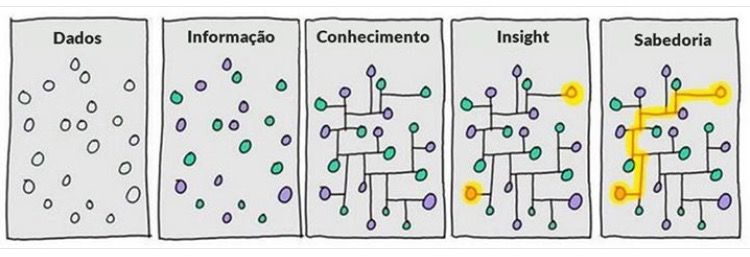
\includegraphics{dados_sabedoria.jpg}

Big Data é basicamente análise de dados. De fato isso não é nenhuma novidade. Há muitos e muitos anos a humanidade coleta dados para serem analisados. A grande inovação está em aliar métodos antigos e limitados de análise de dados aos modernos recursos de hardware de alto processamento. Ou seja, agora é possível transitar todos esses cálculos e análises por meio de softwares desenvolvidos especificamente para trabalharem com enormes quantidades de dados. Uma solução de Big Data funciona com algoritmos complexos que trabalham a informação de modo a obter como saída os mais diversos tipos de insights.

A Análise Descritiva é a fase inicial deste processo de estudo dos dados coletados. Utilizamos métodos de Estatística Descritiva para organizar, resumir e descrever os aspectos importantes de um conjunto de características observadas ou comparar tais características entre dois ou mais conjuntos. As ferramentas descritivas são os muitos tipos de gráficos e tabelas e também medidas de síntese como porcentagens, índices e médias.

Ao se condensar os dados, perde-se informação, pois não se têm as observações originais. Entretanto, esta perda de informação é pequena se comparada ao ganho que se tem com a clareza da interpretação proporcionada.

A descrição dos dados também tem como objetivo identificar anomalias, até mesmo resultante do registro incorreto de valores, e dados dispersos, aqueles que não seguem a tendência geral do restante do conjunto.

Não só nos artigos técnicos direcionados para pesquisadores, mas também nos artigos de jornais e revistas escritos para o público leigo, é cada vez mais frequente a utilização destes recursos de descrição para complementar a apresentação de um fato, justificar ou referendar um argumento.

Durante a pandemia da COVID-19 foram publicadas ótimas visualizações de dados de casos e mortes, mas a mais conhecida delas é o gráfico de John Burn-Murdoch no Financial Times. Esta é uma ótima visualização e ajudou a apresentar gráficos em escala logarítimica para um público amplo.

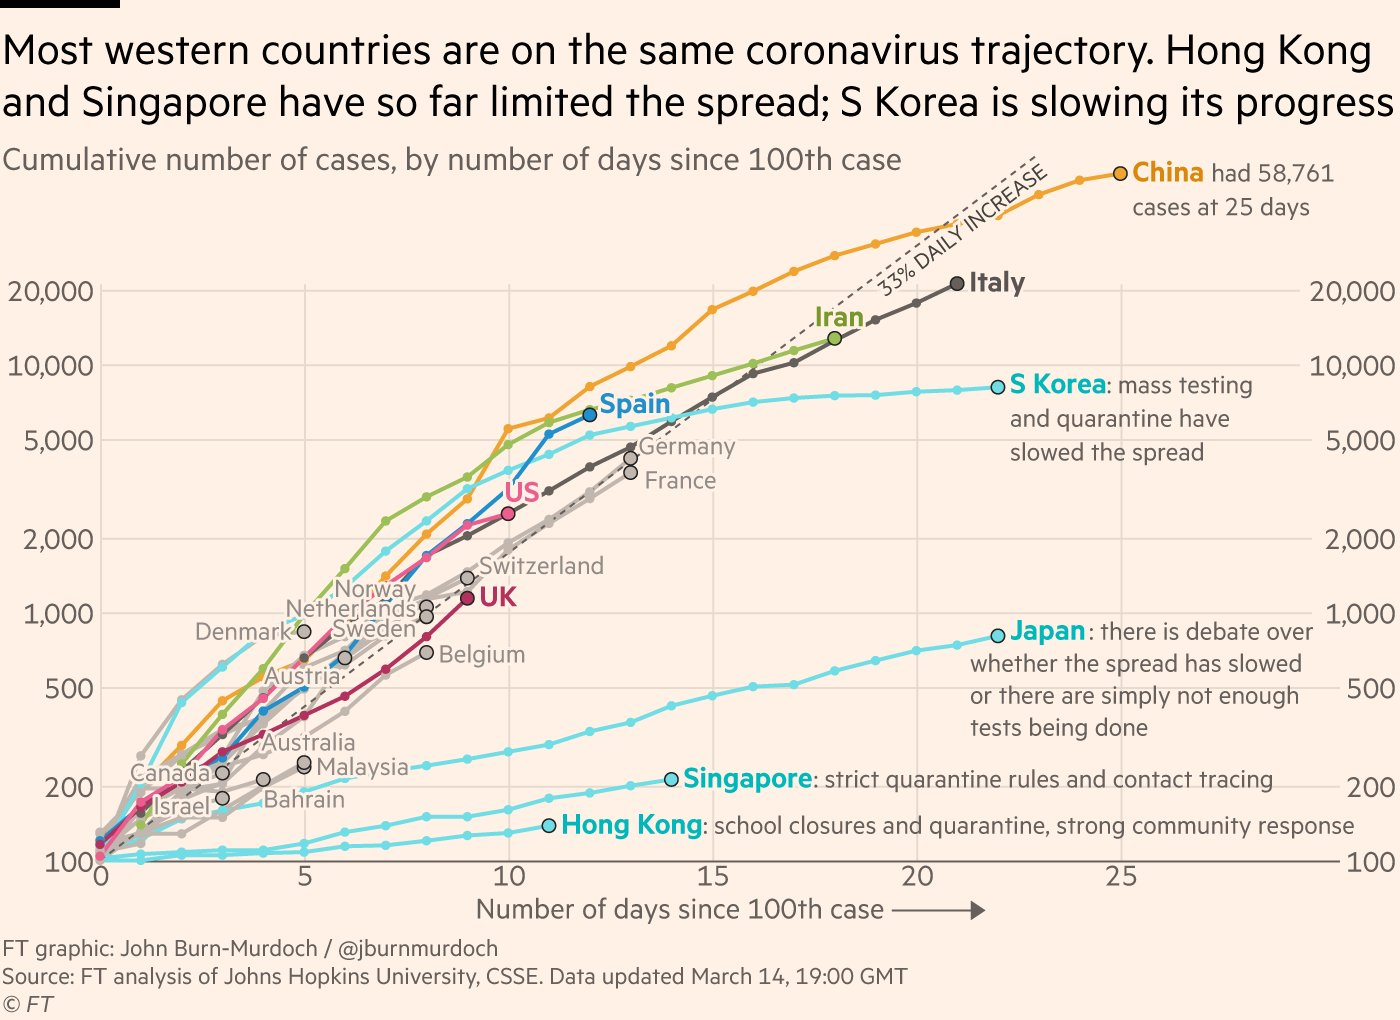
\includegraphics{financial_times.jpg}

Ao mesmo tempo em que o uso das ferramentas estatísticas vem crescendo, aumenta também o abuso de tais ferramentas. É muito comum vermos em jornais e revistas, até mesmo em periódicos científicos, gráficos - voluntariamente ou intencionalmente - enganosos e estatísticas obscuras para justificar argumentos polêmicos.

Neste capítulo iremos mergulhar no mundo da Análise de Descritiva de Dados, explorando estatísticas descritivas e análises gráficas com os pacotes mais atuais do software \(\texttt{R}\) \citep{R2020}.

\hypertarget{coleta-e-armazenamento-de-dados}{%
\section{Coleta e Armazenamento de Dados}\label{coleta-e-armazenamento-de-dados}}

\hypertarget{exemplo-inicial}{%
\subsection{Exemplo inicial}\label{exemplo-inicial}}

O primeiro caso da COVID-19 no Brasil foi confirmado em 25 de fevereiro de 2020, em São Paulo. Desde então o Governo Federal do Brasil reporta diariamente o número total de casos e mortes no país para cada Unidade da Federação, que corresponde aos 26 estados mais o Distrito Federal. No \href{https://github.com/wcota/covid19br}{github do Wesley Cota} \citep{CotaCovid19br2020} é possível extrair tais informações atualizadas para o dia anterior de forma sistematizada numa planilha de dados de maneira a realizar a entrada dos dados num programa de computador.

Para exemplificação, iremos extrair do \href{https://github.com/wcota/covid19br}{github do Wesley Cota} a planilha que possui informações agregadas para o Brasil e suas UFs. Este é o formato mais comum de uma base de dados, composta por linhas e colunas. Cada linha contém os dados de uma Unidade da Federação (elemento) e as informações (variáveis) esntão dispostas nas colunas. Dessa forma, a base de dados contém um número de linhas igual ao número de Unidades da Federação mais o total Brasil e um número de colunas igual ao número de variáveis sendo estudadas.

\begin{tabular}{l|r|r}
\hline
Estado & Casos & Mortes\\
\hline
TOTAL & 26107894 & 630301\\
\hline
AC & 105014 & 1881\\
\hline
AL & 262735 & 6456\\
\hline
AM & 541668 & 13991\\
\hline
AP & 155288 & 2055\\
\hline
BA & 1389564 & 28077\\
\hline
CE & 1160180 & 25450\\
\hline
DF & 625031 & 11208\\
\hline
ES & 897437 & 13607\\
\hline
GO & 1057811 & 25117\\
\hline
MA & 390765 & 10510\\
\hline
MG & 2805771 & 57575\\
\hline
MS & 433787 & 9930\\
\hline
MT & 643879 & 14363\\
\hline
PA & 658777 & 17400\\
\hline
PB & 504216 & 9755\\
\hline
PE & 716733 & 20701\\
\hline
PI & 349140 & 7419\\
\hline
PR & 2042294 & 41334\\
\hline
RJ & 1819607 & 70026\\
\hline
RN & 434608 & 7768\\
\hline
RO & 326272 & 6846\\
\hline
RR & 144582 & 2101\\
\hline
RS & 1885128 & 37041\\
\hline
SC & 1477548 & 20690\\
\hline
SE & 299127 & 6115\\
\hline
SP & 4704552 & 158872\\
\hline
TO & 276380 & 4013\\
\hline
\end{tabular}

Note que se usássemos uma base de dados que contém a evolução da doença por UF então teríamos uma combinação que seria uma linha para cada dia e cada estado, aumentando consideravelmente a dimensão da base.

\hypertarget{tipos-de-variuxe1veis}{%
\section{Tipos de Variáveis}\label{tipos-de-variuxe1veis}}

\textbf{Variável} é a característica de interesse que é medida em cada indivíduo da amostra ou população. Como o nome diz, seus valores variam de indivíduo para indivíduo. As variáveis podem ter valores numéricos ou não numéricos.

\hypertarget{variuxe1veis-quantitativas}{%
\section{Variáveis Quantitativas}\label{variuxe1veis-quantitativas}}

São as características que podem ser medidas em uma escala quantitativa, ou seja, apresentam valores numéricos que fazem sentido. Podem ser contínuas ou discretas.

\begin{itemize}
\tightlist
\item
  \textbf{Variáveis contínuas}: características mensuráveis que assumem valores em uma escala contínua (na reta real), para as quais valores não-inteiros (com casas decimais) fazem sentido. Usualmente devem ser medidas através de algum instrumento.

  \begin{itemize}
  \tightlist
  \item
    Exemplos: peso (balança), altura (régua), tempo (relógio), pressão arterial, idade.
  \end{itemize}
\item
  \textbf{Variáveis discretas}: características mensuráveis que podem assumir apenas um número finito ou infinito contável de valores e, assim, somente fazem sentido valores inteiros. Geralmente, são o resultado de contagens.

  \begin{itemize}
  \tightlist
  \item
    Exemplos: número de filhos, número de bactérias por litro de leite, número de casos de uma doença.
  \end{itemize}
\end{itemize}

\hypertarget{variuxe1veis-qualitativas-ou-categuxf3ricas}{%
\section{Variáveis Qualitativas (ou categóricas)}\label{variuxe1veis-qualitativas-ou-categuxf3ricas}}

São as características que não possuem valores quantitativos, mas, ao contrário, são definidas por várias categorias, ou seja, representam uma classificação dos indivíduos. Podem ser nominais ou ordinais.

\begin{itemize}
\tightlist
\item
  \textbf{Variáveis nominais}: não existe ordenação entre as categorias. Exemplos: sexo, cor dos olhos, fumante/não fumante, doente/sadio.
\item
  \textbf{Variáveis ordinais}: existe uma ordenação entre as categorias. Exemplos: escolaridade (1o, 2o, 3o graus), estágio da doença (inicial,intermediário, terminal), mês de observação (janeiro, fevereiro,\(\ldots\), dezembro).
\end{itemize}

Uma variável originalmente quantitativa pode ser coletada de forma qualitativa. Por exemplo, a variável idade, medida em anos completos, é quantitativa (contínua); mas, se for informada apenas a faixa etária (0 a 5 anos, 6 a 10 anos etc.), é qualitativa (ordinal). Outro exemplo é o peso dos lutadores de boxe, uma variável quantitativa (contínua) se trabalhamos com o valor obtido na balança, mas qualitativa (ordinal) se o classificarmos nas categorias do boxe (peso-pena, peso-leve, peso-pesado etc.).

Outro ponto importante é que nem sempre uma variável representada por números é quantitativa. O número do telefone de uma pessoa, o número da casa, o número de sua identidade. Às vezes o sexo do indivíduo é registrado na planilha de dados como 1 se macho e 2 se fêmea, por exemplo. Isto não significa que a variável sexo passou a ser quantitativa.

\hypertarget{medidas-de-tenduxeancia-central}{%
\section{Medidas de Tendência Central}\label{medidas-de-tenduxeancia-central}}

A tendência central de uma variável em um conjunto de dados é caracterizada pelo valor típico dessa variável. Essa é uma maneira de resumir a informação contida nos dados, pois escolheremos um valor para representar todos os outros. Assim, poderíamos perguntar, por exemplo, qual é a altura típica dos brasileiros adultos no final da década de 90 e compará-la com o valor típico da altura dos brasileiros no final da década de 80, a fim de verificar se os brasileiros estão se tornando, em geral, mais altos, mais baixos ou não sofreram nenhuma alteração em sua altura típica. Fazer essa comparação utilizando medidas-resumo (as alturas típicas em cada período) é bem mais sensato do que comparar os dois conjuntos de dados valor a valor, o que seria inviável. Mas, como identificar o valor típico de um conjunto de dados?

Existem três medidas que podem ser utilizadas para descrever a tendência central de um conjunto de dados: a média, a mediana e a moda. Apresentaremos essas três medidas e discutiremos suas vantagens e desvantagens.

\hypertarget{muxe9dia-aritmuxe9tica-simples}{%
\subsection{Média Aritmética Simples}\label{muxe9dia-aritmuxe9tica-simples}}

A média aritmética simples (que chamaremos apenas de média) é a medida de tendência central mais conhecida e usada para o resumo de dados. Essa popularidade pode ser devida à facilidade de cálculo e à idéia simples que ela nos sugere. De fato, se queremos um valor que represente a altura dos brasileiros adultos, por que não medir as alturas de uma amostra de brasileiros adultos, somar os valores e dividir esse ``bolo'' igualmente entre os participantes? Essa é a idéia da média aritmética.

Para apresentar a média, primeiramente vamos definir alguma notação. A princípio, essa notação pode parecer desnecessária, mas facilitará bastante nosso trabalho futuro.

\begin{equation*}
\text{Notação} 
    \begin{cases}
      n          & \text{tamanho da amostra} \\
      x_i        & \text{valor da $i$-ésima observação} \\
      \sum_{i=1}^n x & \text{soma de todas as observações} \\
      \bar x     & \text{símbolo que representa a média aritmética simples}
    \end{cases}
\end{equation*}

Assim,

\begin{equation*}
\bar x = \frac{\text{soma de todas as observações}}{{n}} = \frac{\sum_{i=1}^n x}{n}
\end{equation*}

Exemplo: No conjunto de dados (1.3, 0.7, 5.8, 2.4, 1.2), temos \(n=5\), \(x_1=\) 1.3, \(x_2=\) 0.7, \(x_3=\) 5.8, \(x_4=\) 2.4 e \(x_5=\) 1.2, portanto \(\sum_{i=1}^5 x_i=\) 1.3 + 0.7 + 5.8 + 2.4 + 1.2 \(=\) 11.4 e assim \(\bar x = \frac{11.4}{5}=2.28\).

Se esses seis valores representassem, por exemplo, as quantidades de peixe pescado (em toneladas) durante cinco dias da semana, a quantidade típica pescada por dia, naquela semana, seria 2,28 toneladas. Como estamos representando o valor típico pela média aritmética, podemos falar em quantidade média diária naquela semana.

Fazendo no \(\texttt{R}\):

\begin{Shaded}
\begin{Highlighting}[]
\FunctionTok{mean}\NormalTok{(}\FunctionTok{c}\NormalTok{(}\FloatTok{1.3}\NormalTok{, }\FloatTok{0.7}\NormalTok{, }\FloatTok{5.8}\NormalTok{, }\FloatTok{2.4}\NormalTok{, }\FloatTok{1.2}\NormalTok{))}
\end{Highlighting}
\end{Shaded}

\begin{verbatim}
## [1] 2.28
\end{verbatim}

\hypertarget{mediana}{%
\subsection{Mediana}\label{mediana}}

A mediana de um conjunto de dados é definida como sendo o ``valor do meio'' desse conjunto de dados, dispostos em ordem crescente, deixando metade dos valores acima dela e metade dos valores abaixo dela.

Como calcular a mediana? Basta seguir sua definição. Vejamos:

\begin{itemize}
\tightlist
\item
  \textbf{\(n\) é ímpar}: Existe apenas um ``valor do meio'', que é a mediana.

  \begin{itemize}
  \tightlist
  \item
    Seja o conjunto de dados (1.3, 0.7, 5.8, 2.4, 1.2).
  \item
    Ordenando os valores (0.7, 1.2, 1.3, 2.4, 5.8).
  \item
    O valor do meio é o 1.3.
  \item
    A mediana é o valor 1.3.
  \end{itemize}
\item
  \textbf{\(n\) é par}: Existem dois ``valores do meio''. A mediana é a média aritmética simples deles.

  \begin{itemize}
  \tightlist
  \item
    Seja o conjunto de dados (1.3, 0.7, 5.8, 2.4, 1.2, 2.1).
  \item
    Ordenando os valores (0.7, 1.2, 1.3, 2.1, 2.4, 5.8).
  \item
    Os valores do meio são 1.3 e 2.1.
  \item
    A mediana é (1.3+2.1)/2=1.7.
  \end{itemize}
\end{itemize}

Fazendo no \(\texttt{R}\):

\begin{Shaded}
\begin{Highlighting}[]
\FunctionTok{median}\NormalTok{(}\FunctionTok{c}\NormalTok{(}\FloatTok{1.3}\NormalTok{, }\FloatTok{0.7}\NormalTok{, }\FloatTok{5.8}\NormalTok{, }\FloatTok{2.4}\NormalTok{, }\FloatTok{1.2}\NormalTok{))}
\end{Highlighting}
\end{Shaded}

\begin{verbatim}
## [1] 1.3
\end{verbatim}

\begin{Shaded}
\begin{Highlighting}[]
\FunctionTok{median}\NormalTok{(}\FunctionTok{c}\NormalTok{(}\FloatTok{1.3}\NormalTok{, }\FloatTok{0.7}\NormalTok{, }\FloatTok{5.8}\NormalTok{, }\FloatTok{2.4}\NormalTok{, }\FloatTok{1.2}\NormalTok{, }\FloatTok{2.1}\NormalTok{))}
\end{Highlighting}
\end{Shaded}

\begin{verbatim}
## [1] 1.7
\end{verbatim}

Como medida de tendência central, a mediana é até mais intuitiva do que a média, pois representa, de fato, o centro (meio) do conjunto de valores ordenados. Assim como a média, o valor da mediana não precisa coincidir com algum dos valores do conjunto de dados. Em particular, quando os dados forem de natureza contínua, essa coincidência dificilmente ocorrerá.

\hypertarget{moda}{%
\subsection{Moda}\label{moda}}

Uma maneira alternativa de representar o que é ``típico'' é através do valor mais frequente da variável, chamado de moda.

Como calcular a moda? Basta verificar o valor que ``aparece'' mais vezes. Vejamos:

\begin{itemize}
\tightlist
\item
  No conjunto de dados (1, 2, 3, 3, 4, 5, 5, 5, 5, 5), há apenas uma moda, o valor \(5\), portanto o conjunto de dados é \textbf{unimodal}.
\item
  No conjunto de dados (1, 2, 2, 2, 2, 3, 4, 5, 6, 6, 6, 6, 7, 9), existem duas modas, os valores \(2\) e \(6\), portanto o conjunto de dados é \textbf{bimodal}.
\item
  Nem sempre a moda existe ou faz sentido, no conjunto de dados (1, 2, 3, 4, 5, 6, 7, 8, 9), não existe um valor mais frequente que os demais, portanto o conjunto de dados é \textbf{amodal}.
\end{itemize}

Para usar a função que calcula a moda (\(\texttt{Mode}\)) no \(\texttt{R}\) temos que instalar e carregar o pacote \(\texttt{pracma}\):

\begin{Shaded}
\begin{Highlighting}[]
\FunctionTok{library}\NormalTok{(pracma)}
\FunctionTok{Mode}\NormalTok{(}\FunctionTok{c}\NormalTok{(}\DecValTok{1}\NormalTok{,}\DecValTok{2}\NormalTok{,}\DecValTok{3}\NormalTok{,}\DecValTok{3}\NormalTok{,}\DecValTok{4}\NormalTok{,}\DecValTok{5}\NormalTok{,}\DecValTok{5}\NormalTok{,}\DecValTok{5}\NormalTok{,}\DecValTok{5}\NormalTok{,}\DecValTok{5}\NormalTok{))}
\end{Highlighting}
\end{Shaded}

\begin{verbatim}
## [1] 5
\end{verbatim}

\begin{Shaded}
\begin{Highlighting}[]
\FunctionTok{Mode}\NormalTok{(}\FunctionTok{c}\NormalTok{(}\DecValTok{1}\NormalTok{,}\DecValTok{2}\NormalTok{,}\DecValTok{2}\NormalTok{,}\DecValTok{2}\NormalTok{,}\DecValTok{2}\NormalTok{,}\DecValTok{3}\NormalTok{,}\DecValTok{4}\NormalTok{,}\DecValTok{5}\NormalTok{,}\DecValTok{6}\NormalTok{,}\DecValTok{6}\NormalTok{,}\DecValTok{6}\NormalTok{,}\DecValTok{6}\NormalTok{,}\DecValTok{7}\NormalTok{,}\DecValTok{9}\NormalTok{)) }\CommentTok{\# escolherá o menor valor, caso haja empate}
\end{Highlighting}
\end{Shaded}

\begin{verbatim}
## [1] 2
\end{verbatim}

\begin{Shaded}
\begin{Highlighting}[]
\FunctionTok{Mode}\NormalTok{(}\FunctionTok{c}\NormalTok{(}\DecValTok{1}\NormalTok{,}\DecValTok{2}\NormalTok{,}\DecValTok{3}\NormalTok{,}\DecValTok{4}\NormalTok{,}\DecValTok{5}\NormalTok{,}\DecValTok{6}\NormalTok{,}\DecValTok{7}\NormalTok{,}\DecValTok{8}\NormalTok{,}\DecValTok{9}\NormalTok{))}
\end{Highlighting}
\end{Shaded}

\begin{verbatim}
## [1] 1
\end{verbatim}

A moda é também a única das medidas de tendência central que faz sentido no caso de variáveis qualitativas. Assim, a categoria dessas variáveis que aparecer com maior freqüência é chamada de categoria modal.

\hypertarget{medidas-de-variabilidade}{%
\section{Medidas de Variabilidade}\label{medidas-de-variabilidade}}

As medidas de tendência central (média, mediana, moda) conseguem resumir em um único número, o valor que é ``típico'' no conjunto de dados. Mas, será que, somente com essas medidas, conseguimos descrever adequadamente o que ocorre em um conjunto de dados?

Vejamos um exemplo: quando pesamos algo em uma balança, esperamos que ela nos dê o verdadeiro peso daquilo que estamos pesando. No entanto, se fizermos várias medições do peso de um mesmo objeto em uma mesma balança, teremos diferentes valores para o peso deste objeto. Ou seja, existe variabilidade nas medições de peso fornecidas pela balança. Neste caso, quanto menor a variabilidade desses valores, mais precisa é a balança (considerando que a média das medidas de peso coincida como seu valor real). Observe na Figura abaixo, onde estão representadas as distribuições das medições do peso de uma esfera de 1000g, feitas por duas balanças (A e B). As duas balanças registram o mesmo peso médio de 1000g (média dos pesos de todas as medições feitas). Isto é, as duas balanças tipicamente acertam o verdadeiro peso da esfera. Porém, pela Figura, podemos notar que

\begin{itemize}
\tightlist
\item
  as medições da balança A \emph{variam pouco} em torno de 1000g: oscilam bastante entre cerca de 950g e 1050g (uma ``imprecisão'' de 50g)
\item
  as medições da balança B \emph{variam muito} em torno de 1000g: oscilam basicamente entre 900g e 1100g (uma ``imprecisão'' de 100g)
\end{itemize}

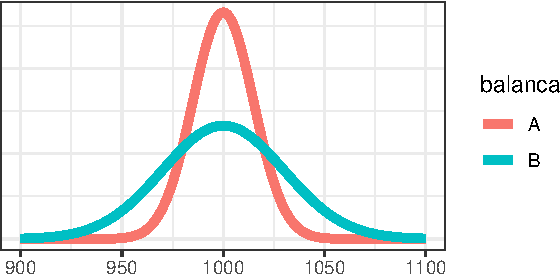
\includegraphics{inferencia_com_R_files/figure-latex/unnamed-chunk-9-1.pdf}

Dois conjuntos de dados podem ter a mesma medida de centro (valor típico), porém uma dispersão diferente em torno desse valor. Desse modo, além de uma medida que nos diga qual é o valor ``típico'' do conjunto de dados, precisamos de uma medida do grau de dispersão (variabilidade) dos dados em torno do valor típico.

O objetivo das medidas de variabilidade é quantificar esse grau de dispersão. Nesta seção, apresentaremos três dessas medidas (amplitude total, desvio-padrão e coeficiente de variação), discutindo suas vantagens e desvantagens. Em discussões posteriores, apresentaremos medidas de variabilidade alternativas.

\hypertarget{amplitude-total}{%
\subsection{Amplitude Total}\label{amplitude-total}}

A medida de variabilidade mais simples é a chamada amplitude total (AT), que é a diferença entre o valor máximo e o valor mínimo de um conjunto de dados.

\begin{equation*}
AT = \text{Máximo}-\text{Mínimo}
\end{equation*}

Exemplo: Medição do peso de uma esfera de 1000g em duas balanças (A e B).

\begin{longtable}[]{@{}lll@{}}
\toprule
Estatísticas & Balança A & Balança B \\
\midrule
\endhead
Mínimo & 945g & 895g \\
Máximo & 1040g & 1095g \\
AT & 1040-945=95g & 1095-895=200g \\
\bottomrule
\end{longtable}

A variabilidade das medições de peso da balança B é maior que a variabilidade das medições de peso da balança A (apesar do valor médio ser igual).

Embora seja uma medida simples de variabilidade, a amplitude total é um tanto grosseira, pois depende somente de dois valores do conjunto de dados (máximo e mínimo), não captando o que ocorre com os outros valores.

Fazendo no \(\texttt{R}\):

\begin{Shaded}
\begin{Highlighting}[]
\DecValTok{1040{-}945}
\end{Highlighting}
\end{Shaded}

\begin{verbatim}
## [1] 95
\end{verbatim}

\begin{Shaded}
\begin{Highlighting}[]
\DecValTok{1095{-}895}
\end{Highlighting}
\end{Shaded}

\begin{verbatim}
## [1] 200
\end{verbatim}

\hypertarget{desvio-padruxe3o}{%
\subsection{Desvio Padrão}\label{desvio-padruxe3o}}

Uma boa medida de dispersão deve considerar todos os valores do conjunto de dados e resumir o grau de dispersão desses valores em torno do valor típico.

Considerando a média como a medida de tendência central, podemos pensar em medir a dispersão (desvio) de cada valor do conjunto de dados em relação à ela. A medida mais simples de desvio entre duas quantidades é a diferença entre elas. Assim, para cada valor \(x_i\), teremos o seu desvio em relação à \(\bar x\) representado por \((x_i-\bar x)\).

Exemplo: No conjunto de dados 1, 1, 2, 3, 4, 4, 5, 6, 7, 7, relativo ao número de filhos de 10 mulheres, temos \(\bar x = 4\) filhos. Na tabela abaixo, a coluna 1 mostra esses 10 valores e a coluna 2 mostra o desvio de cada um deles até a média.

\begin{tabular}{l|l|l}
\hline
Coluna 1 (Xi) & Coluna 2 (Xi-Media) & Coluna 3 (Xi-Media)\textasciicircum{}2\\
\hline
1 & -3 & 9\\
\hline
1 & -3 & 9\\
\hline
2 & -2 & 4\\
\hline
3 & -1 & 1\\
\hline
4 & 0 & 0\\
\hline
4 & 0 & 0\\
\hline
5 & 1 & 1\\
\hline
6 & 2 & 4\\
\hline
7 & 3 & 9\\
\hline
7 & 3 & 9\\
\hline
Soma & 0 & 46\\
\hline
\end{tabular}

\textbf{A ideia do desvio padrão}

Como temos um desvio para cada elemento, poderíamos pensar em resumi-los em um desvio típico, a exemplo do que fizemos com a média. Porém, quando somarmos esses desvios para o cálculo do desvio médio, a soma dará sempre zero, como pode ser visto na coluna 2 do exemplo anterior. Isto ocorre com qualquer conjunto de dados, pois os desvios negativos sempre compensaram os positivos.

No entanto, os sinais dos desvios não são importantes para nossa medida de dispersão, já que estamos interessados na quantidade de dispersão e não na direção dela. Portanto, eliminaremos os sinais elevando os desvios ao quadrado, como mostrado na coluna 3. A soma desses desvios ao quadrado pode ser, então, dividida entre os participantes do ``bolo''. Na verdade, por razões absolutamente teóricas, dividiremos essa soma pelo total de participantes menos 1 \((n-1)\). Assim, usando a notação definida anteriormente, teremos

\begin{equation*}
\frac{\sum_{i=1}^n (x_i-\bar x)^2}{n-1}
\end{equation*}

Para os dados do exemplo, teremos \(46/(10-1)=5,11\). Esse valor pode ser visto como uma quase-média dos desvios ao quadrado e é chamado de \textbf{variância}.

A variância seria nossa medida de variabilidade se não fosse o fato de que ela está expressa em uma unidade diferente da unidade dos dados, pois, ao elevarmos os desvios ao quadrado, elevamos também as unidades de medida em que eles estão expressos. No caso dos dados do exemplo, medidos em número de filhos, a variância vale \(5,11\) ``filhos ao quadrado'', algo que não faz nenhum sentido.

Para eliminar esse problema, extraímos a raiz quadrada da variância e, finalmente, temos a nossa medida de variabilidade, que chamaremos desvio-padrão (DP).

\begin{equation*}
DP=\sqrt{\frac{\sum_{i=1}^n (x_i-\bar x)^2}{n-1}}
\end{equation*}

O desvio-padrão, como o nome já diz, representa o desvio típico dos dados em relação à média, escolhida como medida de tendência central. No exemplo, temos que o desvio padrão vale \(2,26\). Isto significa que a distância típica (padrão) de cada mãe até o número médio de filhos (4 filhos) é de 2,26 filhos. Quanto maior o desvio-padrão, mais diferentes entre si serão as quantidades de filhos de cada mãe.

O desvio-padrão, em alguns livros chamado de \(s\), é uma medida sempre positiva. Se observarmos a maneira como ele é calculado, veremos que não há como obter um valor
negativo.

Fazendo no \(\texttt{R}\):

\begin{Shaded}
\begin{Highlighting}[]
\FunctionTok{round}\NormalTok{(}\FunctionTok{var}\NormalTok{(}\FunctionTok{c}\NormalTok{(}\DecValTok{1}\NormalTok{,}\DecValTok{1}\NormalTok{,}\DecValTok{2}\NormalTok{,}\DecValTok{3}\NormalTok{,}\DecValTok{4}\NormalTok{,}\DecValTok{4}\NormalTok{,}\DecValTok{5}\NormalTok{,}\DecValTok{6}\NormalTok{,}\DecValTok{7}\NormalTok{,}\DecValTok{7}\NormalTok{)),}\DecValTok{2}\NormalTok{) }\CommentTok{\# função round() serve para arrendondar o número de dígitos}
\end{Highlighting}
\end{Shaded}

\begin{verbatim}
## [1] 5.11
\end{verbatim}

\begin{Shaded}
\begin{Highlighting}[]
\FunctionTok{round}\NormalTok{(}\FunctionTok{sd}\NormalTok{(}\FunctionTok{c}\NormalTok{(}\DecValTok{1}\NormalTok{,}\DecValTok{1}\NormalTok{,}\DecValTok{2}\NormalTok{,}\DecValTok{3}\NormalTok{,}\DecValTok{4}\NormalTok{,}\DecValTok{4}\NormalTok{,}\DecValTok{5}\NormalTok{,}\DecValTok{6}\NormalTok{,}\DecValTok{7}\NormalTok{,}\DecValTok{7}\NormalTok{)),}\DecValTok{2}\NormalTok{)}
\end{Highlighting}
\end{Shaded}

\begin{verbatim}
## [1] 2.26
\end{verbatim}

Exemplo: Os agentes de fiscalização de certo município realizam, periodicamente, uma vistoria nos bares e restaurantes para apurar possíveis irregularidades na venda de seus produtos. A seguir, são apresentados dados de uma vistoria sobre os pesos (em gramas) de uma amostra de 10 bifes, constantes de um cardápio de um restaurante como ``bife de 200 gramas''.

\begin{verbatim}
##  [1] 170 175 180 185 190 195 200 200 200 205
\end{verbatim}

Como podemos notar, nem todos os ``bifes de 200 gramas'' pesam realmente 200 gramas. Esta variação é natural e é devida ao processo de produção dos bifes. No entanto, esses bifes deveriam pesar cerca de 200 gramas e com pouca variação em torno desse valor. Com o auxílio do \(\texttt{R}\), calcularemos a média e o desvio-padrão.

\begin{Shaded}
\begin{Highlighting}[]
\FunctionTok{mean}\NormalTok{(}\FunctionTok{c}\NormalTok{(}\DecValTok{170}\NormalTok{,}\DecValTok{175}\NormalTok{,}\DecValTok{180}\NormalTok{,}\DecValTok{185}\NormalTok{,}\DecValTok{190}\NormalTok{,}\DecValTok{195}\NormalTok{,}\DecValTok{200}\NormalTok{,}\DecValTok{200}\NormalTok{,}\DecValTok{200}\NormalTok{,}\DecValTok{205}\NormalTok{))}
\end{Highlighting}
\end{Shaded}

\begin{verbatim}
## [1] 190
\end{verbatim}

\begin{Shaded}
\begin{Highlighting}[]
\FunctionTok{sd}\NormalTok{(}\FunctionTok{c}\NormalTok{(}\DecValTok{170}\NormalTok{,}\DecValTok{175}\NormalTok{,}\DecValTok{180}\NormalTok{,}\DecValTok{185}\NormalTok{,}\DecValTok{190}\NormalTok{,}\DecValTok{195}\NormalTok{,}\DecValTok{200}\NormalTok{,}\DecValTok{200}\NormalTok{,}\DecValTok{200}\NormalTok{,}\DecValTok{205}\NormalTok{))}
\end{Highlighting}
\end{Shaded}

\begin{verbatim}
## [1] 12.0185
\end{verbatim}

Os bifes desse restaurante pesam, em média, 190 gramas, com um desvio-padrão de 12 gramas. Ou seja, os pesos dos ``bifes de 200 gramas'' variam tipicamente entre 178 e 202 gramas. Analisando esses valores, concluímos que esse restaurante pode estar lesando a maior parte de seus clientes.

Para casos como esse, os agentes fiscalizadores podem estabelecer parâmetros (valores) para saber até quanto a média pode se desviar do valor correto e o quanto de variação eles podem permitir numa amostra para concluir que o processo de produção de bifes não possui problemas. Por exemplo, a média da amostra não poderia ser inferior a 198 gramas, com um desvio-padrão que não seja superior a 5\% dessa média.

Essas idéias são utilizadas no controle do processo de produção das indústrias, onde já se espera alguma variação entre as unidades produzidas. Porém, essa variação deve estar sob controle. Numa indústria farmacêutica, por exemplo, espera-se que os comprimidos de uma certa droga sejam produzidos com uma certa variação em sua composição (maior ou menor quantidade do princípio ativo), devido à própria maneira como os comprimidos são produzidos (máquinas, pessoas etc.). No entanto, esta variação deve ser pequena, para que não sejam produzidos comprimidos inócuos (com pouco do princípio ativo) ou com extra-dosagem do princípio ativo, o que, em ambos os casos, pode causar sérias complicações à saúde do paciente.

O desvio-padrão nos permite distinguir numericamente conjuntos de dados de mesmo tamanho, mesma média, mas que são visivelmente diferentes. Usando o desvio-padrão, também conseguimos representar numericamente a variabilidade das medições das balanças A e B, que, apesar de possuírem a mesma média, possuem variabilidades bastante diferentes.

Quando os conjuntos de dados a serem comparados possuem médias diferentes, a comparação da variabilidade desses conjuntos deve levar em conta essa diferença. Por esta e outras razões, definiremos uma terceira medida de variabilidade, o \textbf{coeficiente de variação}.

\hypertarget{coeficiente-de-variauxe7uxe3o}{%
\subsection{Coeficiente de Variação}\label{coeficiente-de-variauxe7uxe3o}}

Ao analisarmos o grau de dispersão de um conjunto de dados, poderemos nos deparar com uma questão do tipo: um desvio-padrão de 10 unidades é pequeno ou grande?

Vejamos:

\begin{itemize}
\tightlist
\item
  Se estivermos trabalhando com um conjunto de dados cuja média é 10.000, um desvio típico de 10 unidades em torno dessa média significa pouca dispersão;
\item
  Mas, se a média for igual a 100, um desvio típico de 10 unidades em torno dessa média significa muita dispersão.
\end{itemize}

Assim, antes de responder se um desvio-padrão de 10 unidades é grande ou pequeno, devemos avaliar sua magnitude em relação à média:

\begin{itemize}
\tightlist
\item
  No primeiro caso, o desvio-padrão corresponde a 0,1\% da média
\item
  No segundo caso, o desvio-padrão corresponde a 10\% da média
\end{itemize}

À essa razão entre o desvio-padrão e a média damos o nome de \textbf{Coeficiente de Variação}:

\begin{equation*}
CV=\frac{\text{Desvio Padrão}}{\text{Média}}
\end{equation*}

Quanto menor o Coeficiente de Variação de um conjunto de dados, menor é a sua variabilidade. O Coeficiente de Variação expressa o quanto da escala de medida, representada pela média, é ocupada pelo desvio-padrão.

O Coeficiente de Variação é uma medida adimensional, isto é, não depende da unidade de medida. Essa característica nos permite usá-lo para comparar a variabilidade de conjuntos de dados medidos em unidades diferentes, o que seria impossível usando o desvio-padrão.

Exemplo: Numa pesquisa na área de Saúde Ocupacional, deseja-se comparar a idade de motoristas e cobradores de ônibus da região metropolitana de Belo Horizonte. Algumas estatísticas descritivas são apresentadas na Tabela abaixo.

\begin{tabular}{l|r|r|r|r}
\hline
Grupo & n & Media & DP & CV\\
\hline
Motoristas & 150 & 35.6 & 5.08 & 0.143\\
\hline
Cobradores & 50 & 22.6 & 3.11 & 0.137\\
\hline
\end{tabular}

Os motoristas são, em média, 13 anos mais velhos do que os cobradores. Ao compararmos o grau de dispersão dos dois grupos usando o desvio-padrão, concluiríamos que os motoristas são menos homogêneos quanto à idade do que os cobradores. Ao fazermos isso, estamos esquecendo que, apesar de estarem em unidades iguais, as medidas de idade nos dois grupos variam em escalas diferentes. As idades dos motoristas variam em torno dos 35 anos e podem chegar até 18 anos (idade mínima para se conseguir a habilitação), numa amplitude de 17 unidades. Enquanto isso, as idades dos cobradores variam em torno de 22 anos e também só podem chegar até a 18 anos, uma amplitude de apenas 4 anos. Assim, os motoristas tem a possibilidade de ter um desvio-padrão maior do que o dos cobradores. Se levarmos em conta a escala de medida, usando o coeficiente de variação, veremos que os motoristas são somente um pouco mais heterogêneos (dispersos) quanto à idade do que os cobradores.

Fazendo no \(\texttt{R}\):

\begin{Shaded}
\begin{Highlighting}[]
\NormalTok{media}\OtherTok{=}\FunctionTok{c}\NormalTok{(}\FloatTok{35.6}\NormalTok{,}\FloatTok{22.6}\NormalTok{)}
\NormalTok{desvio}\OtherTok{=}\FunctionTok{c}\NormalTok{(}\FloatTok{5.08}\NormalTok{,}\FloatTok{3.11}\NormalTok{)}
\FunctionTok{round}\NormalTok{(desvio}\SpecialCharTok{/}\NormalTok{media,}\DecValTok{3}\NormalTok{)}
\end{Highlighting}
\end{Shaded}

\begin{verbatim}
## [1] 0.143 0.138
\end{verbatim}

\hypertarget{medidas-de-posiuxe7uxe3o}{%
\section{Medidas de Posição}\label{medidas-de-posiuxe7uxe3o}}

Quando falamos de posição ou colocação de um indivíduo em uma corrida ou em um teste como o Vestibular, frequentemente nos referimos ao seu posto, como 1º, 2º, 3º, 29º ou último lugar. Mas, para sabermos se uma dada colocação é ou não um bom resultado, precisamos informar quantos indivíduos participaram da corrida ou do Vestibular.

A medida de posição que veremos aqui, os percentis, solucionam este e outros problemas de posicionamento (ranking). A posição de um indivíduo no conjunto de dados é mostrada, pelo percentil, contando-se (em porcentagem) quantos indivíduos do conjunto têm valores menores que o deste indivíduo.

Como veremos, esta medida de posição pode ser usada para comparar a posição do indivíduo em diferentes conjuntos de dados, nos quais foram medidas as mesmas variáveis ou variáveis diferentes.

\hypertarget{percentis}{%
\subsection{Percentis}\label{percentis}}

Considere o trecho a seguir, sobre a posição do Brasil, entre os países do mundo, quanto à renda per capita:

\emph{O Brasil obviamente não é país rico, mas também não está entre os mais pobres. \(\ldots\) Mais de três quartos da população mundial vivem em países de renda per capita menor}

Neste caso, o posição do Brasil é dada pela quantidade de países que têm renda per capita menores que o Brasil, a saber três quartos ou \(75\%\). O mesmo tipo de raciocínio fazemos quando dizemos que certo aluno está entre os \(5\%\) melhores do colégio. Não precisamos nem saber quantos alunos tem o colégio ou em quantos países estão sendo consideradas as rendas. Aqui já houve uma padronização da posição usando-se a porcentagem de alunos ou países com desempenho ou renda abaixo do valor considerado. É este raciocínio que define os percentis.

\textbf{O percentil de ordem $K$ (onde $k$ é qualquer valor entre $0$ e $100$), denotado por $P_k$, é o valor tal que $K\%$ dos valores do conjunto de dados são menores ou iguais a ele.}

Assim, o percentil de ordem \(10\), o \(P_{10}\), é o valor da variável tal que \(10\%\) dos valores são menores ou iguais a ele; o percentil de ordem \(65\) deixa \(65\%\) dos dados menores ou iguais a ele etc.

Os percentil de ordem \(10,20,30,\ldots,90\) dividem o conjunto de dados em dez partes com mesmo número de observações e são chamados de \textbf{decis}.

Os percentis de ordem \(25,50\) e \(75\) dividem o conjunto de dados em quatro partes com o mesmo número de observações. Assim, estes três percentis recebem o nome de quartis -- \textbf{primeiro quartil (Q1), segundo quartil (Q2) e terceiro quartil (Q3)}, respectivamente. O segundo quartil é a já conhecida mediana.

Existem vários processos para calcular os percentis, usando interpolação. Vamos ficar com um método mais simples, mostrado na Figura a seguir. As diferenças serão muito pequenas e desaparecerão à medida que aumenta o número de dados.

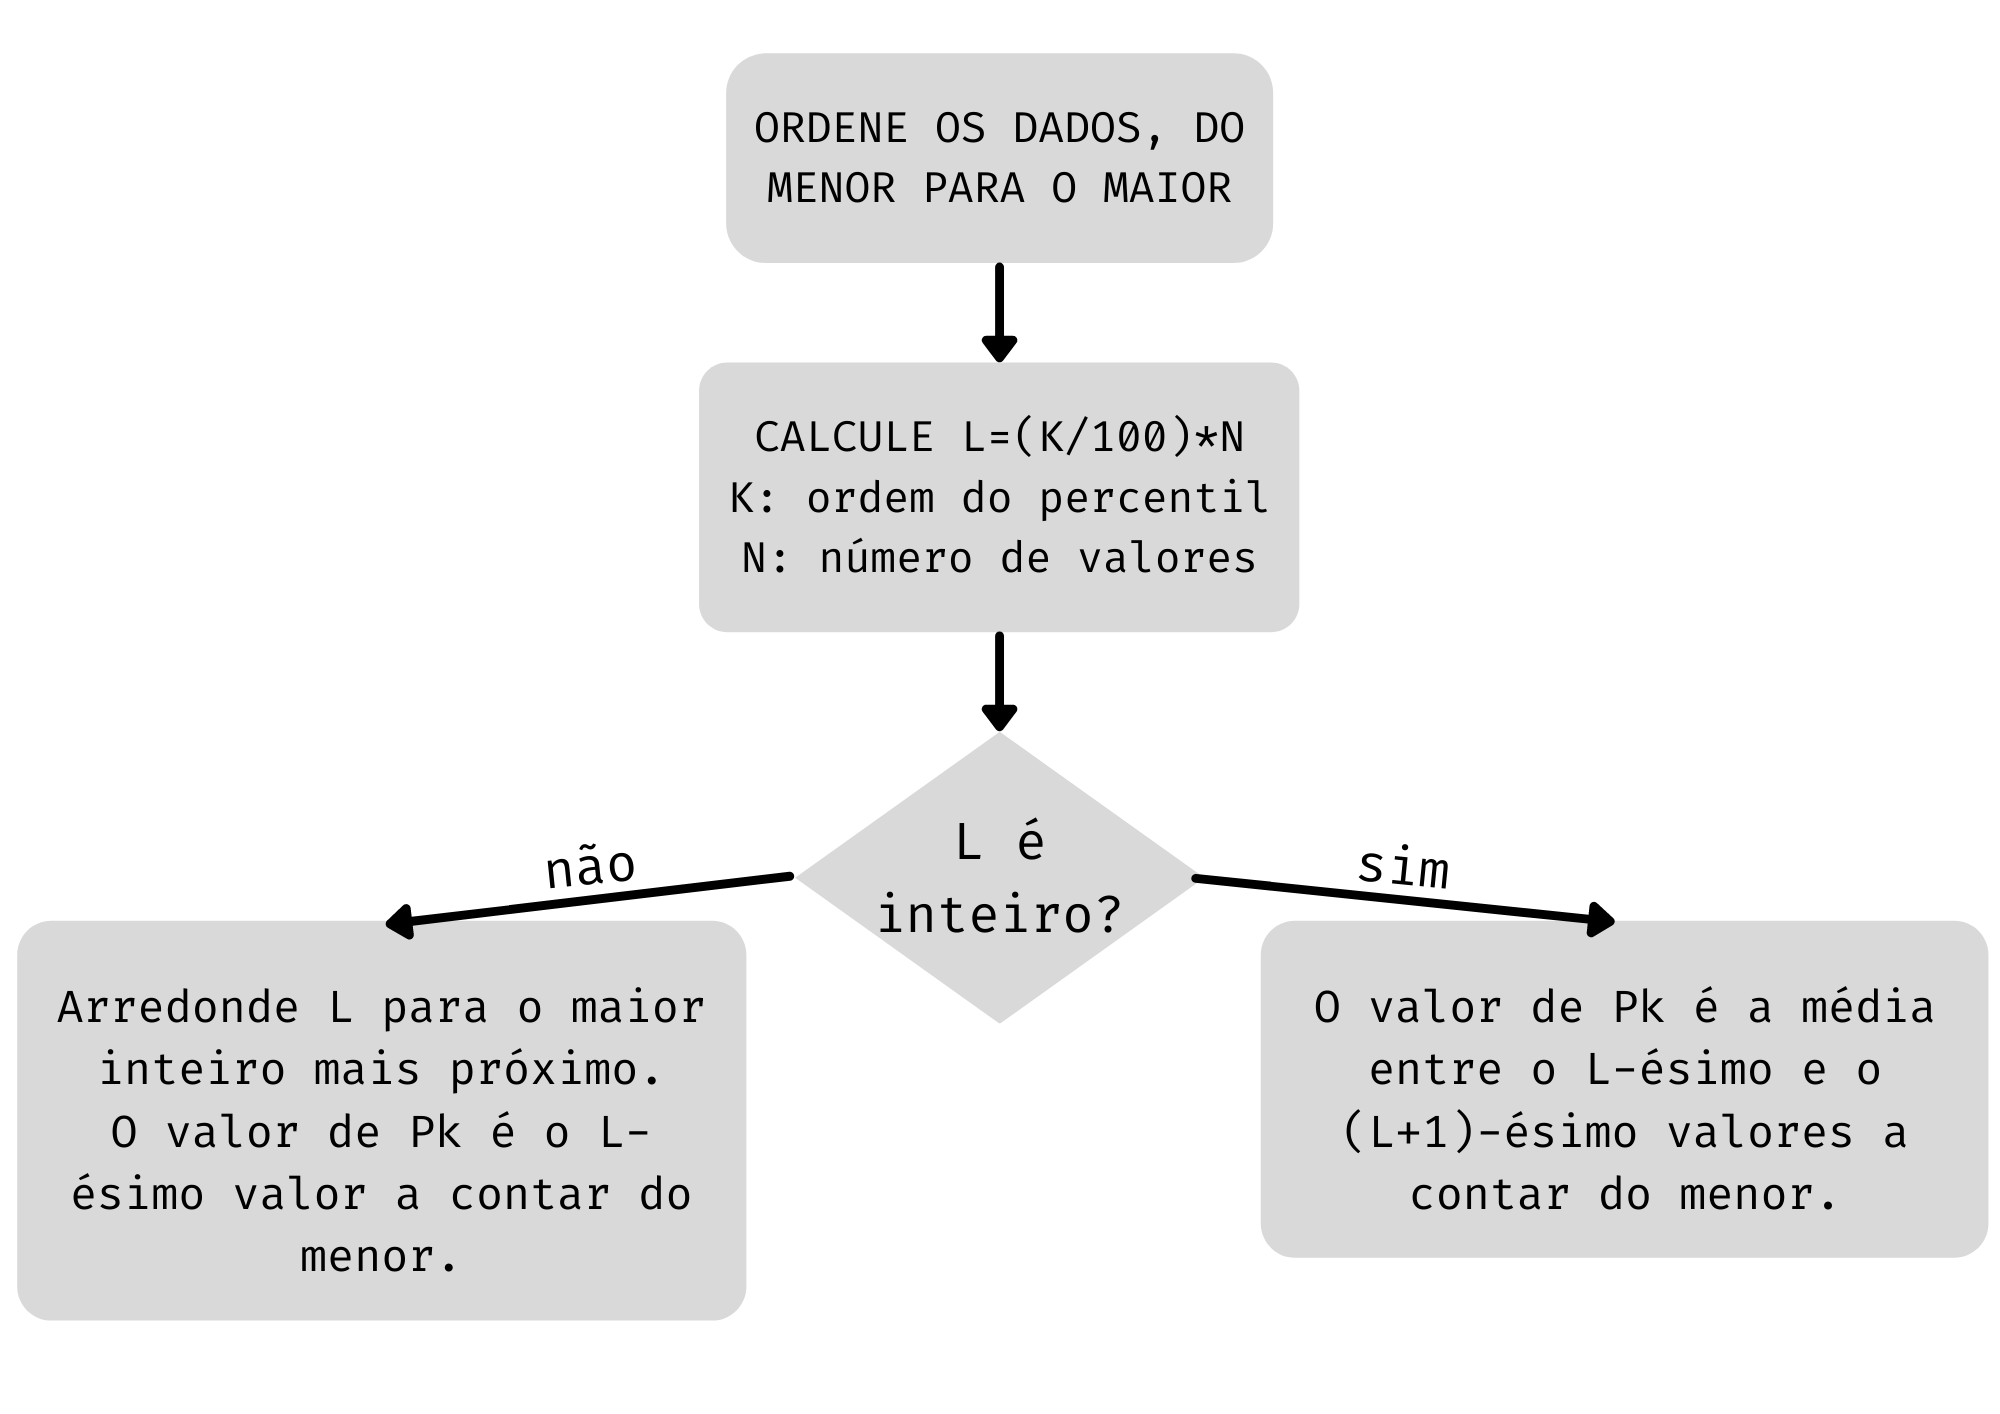
\includegraphics{fluxograma_percentil.png}

Considere as notas finais dos 40 candidatos ao curso de Direito no Vestibular de certa faculdade, já colocadas em ordem crescente:

\begin{verbatim}
##  [1] 40 41 42 42 44 47 48 48 49 49 51 52 53 58 59 62 63 64 65 66 67 68 69 70 75
## [26] 76 83 83 85 86 86 87 87 88 92 93 94 95 97 98
\end{verbatim}

Vamos calcular alguns percentis:

\begin{itemize}
\item
  Percentil de ordem \(10\): \(10\%\) de \(40=4\). Então o \(P_10\) = média(4º e 5º valores)=\((42+44)/2=43\).
\item
  Percentil de ordem \(95\): \(95\%\) de \(40=38\). Então o \(P_95\) = média(38º e 39º valores)=\((95+97)/2=96\).
\item
  Primeiro Quartil: \(25\%\) de \(40=10\). Então o Q1 = média(10º e 11º valores)=\((49+51)/2 = 50\).
\item
  Terceiro Quartil: \(75\%\) de \(40=30\). Então o Q3 = média(30º e 31º valores)=\((86+86)/2 = 86\).
\item
  Mediana: \(50\%\) de \(40=20\). Então mediana = média(20º e 21º valores)=\((66+67)/2 = 66,5\).
\end{itemize}

Fazendo no \(\texttt{R}\):

\begin{Shaded}
\begin{Highlighting}[]
\NormalTok{dados\_ex7}\OtherTok{=}\FunctionTok{c}\NormalTok{(}\DecValTok{40}\NormalTok{,}\DecValTok{41}\NormalTok{,}\DecValTok{42}\NormalTok{,}\DecValTok{42}\NormalTok{,}\DecValTok{44}\NormalTok{,}\DecValTok{47}\NormalTok{,}\DecValTok{48}\NormalTok{,}\DecValTok{48}\NormalTok{,}\DecValTok{49}\NormalTok{,}
            \DecValTok{49}\NormalTok{,}\DecValTok{51}\NormalTok{,}\DecValTok{52}\NormalTok{,}\DecValTok{53}\NormalTok{,}\DecValTok{58}\NormalTok{,}\DecValTok{59}\NormalTok{,}\DecValTok{62}\NormalTok{,}\DecValTok{63}\NormalTok{,}\DecValTok{64}\NormalTok{,}
            \DecValTok{65}\NormalTok{,}\DecValTok{66}\NormalTok{,}\DecValTok{67}\NormalTok{,}\DecValTok{68}\NormalTok{,}\DecValTok{69}\NormalTok{,}\DecValTok{70}\NormalTok{,}\DecValTok{75}\NormalTok{,}\DecValTok{76}\NormalTok{,}\DecValTok{83}\NormalTok{,}
            \DecValTok{83}\NormalTok{,}\DecValTok{85}\NormalTok{,}\DecValTok{86}\NormalTok{,}\DecValTok{86}\NormalTok{,}\DecValTok{87}\NormalTok{,}\DecValTok{87}\NormalTok{,}\DecValTok{88}\NormalTok{,}\DecValTok{92}\NormalTok{,}\DecValTok{93}\NormalTok{,}\DecValTok{94}\NormalTok{,}\DecValTok{95}\NormalTok{,}\DecValTok{97}\NormalTok{,}\DecValTok{98}\NormalTok{)}
\FunctionTok{quantile}\NormalTok{(dados,}\AttributeTok{probs=}\FunctionTok{c}\NormalTok{(}\FloatTok{0.1}\NormalTok{,}\FloatTok{0.95}\NormalTok{,}\FloatTok{0.25}\NormalTok{,}\FloatTok{0.75}\NormalTok{,}\FloatTok{0.5}\NormalTok{))}
\end{Highlighting}
\end{Shaded}

\begin{verbatim}
##    10%    95%    25%    75%    50% 
## 174.50 202.75 181.25 200.00 192.50
\end{verbatim}

Veja que os valores encontrados pelo \(\texttt{R}\) não coincidem com os calculados ``na mão'', isto porque, o \(\texttt{R}\) utiliza um método de interpolação para calcular valores que não estão presentes na amostra.

\hypertarget{referuxeancias}{%
\section{Referências}\label{referuxeancias}}

\hypertarget{anuxe1lise-gruxe1fica}{%
\chapter{Análise Gráfica}\label{anuxe1lise-gruxe1fica}}

\hypertarget{introduuxe7uxe3o-1}{%
\section{Introdução}\label{introduuxe7uxe3o-1}}

Já sabemos que as variáveis de um estudo dividem-se em quatro tipos:

\begin{itemize}
\tightlist
\item
  Qualitativas:

  \begin{itemize}
  \tightlist
  \item
    nominais
  \item
    ordinais
  \end{itemize}
\item
  Quantitativas:

  \begin{itemize}
  \tightlist
  \item
    discretas
  \item
    contínuas
  \end{itemize}
\end{itemize}

Os dados gerados por esses tipos de variáveis são de naturezas diferentes e devem receber tratamentos diferentes. Portanto, vamos estudar as ferramentas mais adequadas para cada tipo de dados, separadamente.

\hypertarget{variuxe1veis-qualitativas---nominais-e-ordinais}{%
\section{Variáveis Qualitativas - Nominais e Ordinais}\label{variuxe1veis-qualitativas---nominais-e-ordinais}}

Na base de dados \(\texttt{mtcars}\), uma das duas variáveis qualitativas presentes é a categoria da transmissão (automática ou manual). Para organizar os dados provenientes de uma variável qualitativa, é usual fazer uma tabela de frequências, como a tabela abaixo, onde estão apresentadas as frequências com que ocorre cada um dos tipos de transmissão no total dos 32 carros observados. Cada categoria da variável transmissão (automática, manual) é representada numa linha da tabela. Há uma coluna com as contagens de carros em cada categoria (frequência absoluta) e outra com os percentuais que essas contagens representam no total de carros (frequência relativa). Esse tipo de tabela representa a distribuição de frequências dos carros segundo a variável transmissão.

Como a variável transmissão é qualitativa nominal, ou seja, não há uma ordem natural em suas categorias, a ordem das linhas da tabela pode ser qualquer uma. É comum a disposição das linhas pela ordem decrescente das frequências das classes.

\begin{tabular}{l>{\raggedleft\arraybackslash}p{2.5cm}>{\raggedleft\arraybackslash}p{2.5cm}}
\toprule
Transmissão & Frequência Absoluta & Frequência Relativa (\%)\\
\midrule
Automático & 19 & 59.38\\
Manual & 13 & 40.62\\
Total & 32 & 100.00\\
\bottomrule
\end{tabular}

Quando a variável tabelada for do tipo qualitativa ordinal, as linhas da tabela de frequências devem ser dispostas na ordem existente para as categorias. A tabela abaixo mostra a distribuição de
frequências das coletas segundo o mês de observação na base de dados \(\texttt{airquality}\), que é uma variável qualitativa ordinal. Nesse caso, podemos acrescentar mais duas colunas com as frequências acumuladas (absoluta e relativa), que mostram, para cada mês, a frequência das coletas até aquele mês. Por exemplo, até o mês de julho, foram coletadas 92 amostras, o que representa 60,13\% do total de amostras coletadas.

\begin{tabular}{l>{\raggedleft\arraybackslash}p{2.5cm}>{\raggedleft\arraybackslash}p{2.5cm}>{\raggedright\arraybackslash}p{2.5cm}>{\raggedright\arraybackslash}p{2.5cm}}
\toprule
Transmissão & Frequência Absoluta & Frequência Relativa (\%) & Frequência Absoluta Acumulada & Frequência Relativa Acumulada (\%)\\
\midrule
5 & 31 & 20.26 & 31 & 20.26\\
6 & 30 & 19.61 & 61 & 39.87\\
7 & 31 & 20.26 & 92 & 60.13\\
8 & 31 & 20.26 & 123 & 80.39\\
9 & 30 & 19.61 & 153 & 100\\
\addlinespace
Total & 153 & 100.00 & - & -\\
\bottomrule
\end{tabular}

Note que as frequências acumuladas não fazem sentido em distribuição de frequências de variáveis para as quais não existe uma ordem natural nas categorias, as qualitativas nominais.

A visualização da distribuição de frequências de uma variável fica mais fácil se fizermos um gráfico a partir da tabela de frequências. Existem vários tipos de gráficos, dependendo do tipo de variável a ser representada. Para as variáveis do tipo qualitativas, abordaremos dois tipos de gráficos: os de setores e os de barras.

Os gráficos de setores, mais conhecidos como gráficos de pizza ou torta, são construídos dividindo-se um círculo (pizza) em setores (fatias), um para cada categoria, que serão proporcionais à frequência daquela categoria.

A Figura a seguir mostra um gráfico de setores para a variável transmissão, construído a partir da primeira tabela de frequências. Através desse gráfico, fica mais fácil perceber que os carros automáticos são a grande maioria dos carros. Como esse gráfico contém todas as informações da tabela, pode substituí-la com a vantagem de tornar análise dessa variável mais agradável.

\begin{Shaded}
\begin{Highlighting}[]
\FunctionTok{library}\NormalTok{(ggplot2)}
\NormalTok{df }\OtherTok{=} \FunctionTok{data.frame}\NormalTok{(}\FunctionTok{table}\NormalTok{(mtcars}\SpecialCharTok{$}\NormalTok{am))}
\FunctionTok{levels}\NormalTok{(df}\SpecialCharTok{$}\NormalTok{Var1) }\OtherTok{=} \FunctionTok{c}\NormalTok{(}\StringTok{"Automático"}\NormalTok{,}\StringTok{"Manual"}\NormalTok{)}
\FunctionTok{ggplot}\NormalTok{(df, }\FunctionTok{aes}\NormalTok{(}\AttributeTok{x=}\StringTok{""}\NormalTok{, }\AttributeTok{y=}\NormalTok{Freq, }\AttributeTok{fill=}\NormalTok{Var1)) }\SpecialCharTok{+}
  \FunctionTok{geom\_bar}\NormalTok{(}\AttributeTok{stat=}\StringTok{"identity"}\NormalTok{) }\SpecialCharTok{+}
  \FunctionTok{coord\_polar}\NormalTok{(}\StringTok{"y"}\NormalTok{, }\AttributeTok{start=}\DecValTok{0}\NormalTok{) }\SpecialCharTok{+}
  \FunctionTok{theme\_void}\NormalTok{() }\SpecialCharTok{+}
  \FunctionTok{theme}\NormalTok{(}\AttributeTok{legend.title =} \FunctionTok{element\_blank}\NormalTok{())}
\end{Highlighting}
\end{Shaded}

\begin{center}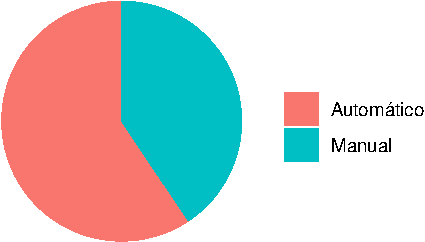
\includegraphics{inferencia_com_R_files/figure-latex/unnamed-chunk-23-1} \end{center}

Quando houver mais de duas categorias de uma variável nominal, a disposição no gráfico de setores deve ser pela ordem decrescente das frequências, no sentido horário. A categoria ``outros'', quando existir, deve ser sempre a última, mesmo não seja a de menor frequência.

As vantagens da representação gráfica das distribuições de frequências ficam ainda mais evidentes quando há a necessidade de comparar vários grupos com relação à variáveis que possuem muitas categorias, como veremos mais adiante.

Uma alternativa ao gráfico de setores é o gráfico de barras (colunas) como o da figura a seguir. Ao invés de dividirmos um círculo, dividimos uma barra. Note que, em ambos os gráficos, as frequências relativas das categorias devem somar 100\%. Aliás, esse é a idéia dos gráficos: mostrar como se dá a divisão (distribuição) do total de elementos (100\%) em partes (fatias).

\begin{Shaded}
\begin{Highlighting}[]
\NormalTok{df }\OtherTok{=} \FunctionTok{data.frame}\NormalTok{(}\FunctionTok{table}\NormalTok{(mtcars}\SpecialCharTok{$}\NormalTok{am))}
\FunctionTok{levels}\NormalTok{(df}\SpecialCharTok{$}\NormalTok{Var1) }\OtherTok{=} \FunctionTok{c}\NormalTok{(}\StringTok{"Automático"}\NormalTok{,}\StringTok{"Manual"}\NormalTok{)}
\FunctionTok{ggplot}\NormalTok{(df, }\FunctionTok{aes}\NormalTok{(}\AttributeTok{x=}\NormalTok{Var1, }\AttributeTok{y=}\NormalTok{Freq, }\AttributeTok{fill=}\NormalTok{Var1)) }\SpecialCharTok{+}
  \FunctionTok{geom\_bar}\NormalTok{(}\AttributeTok{stat=}\StringTok{"identity"}\NormalTok{) }\SpecialCharTok{+}
  \FunctionTok{geom\_text}\NormalTok{(}\FunctionTok{aes}\NormalTok{(}\AttributeTok{label =}\NormalTok{ Freq),}\AttributeTok{position=}\FunctionTok{position\_stack}\NormalTok{(}\AttributeTok{vjust =} \FloatTok{0.5}\NormalTok{)) }\SpecialCharTok{+}
  \FunctionTok{theme}\NormalTok{(}\AttributeTok{legend.title =} \FunctionTok{element\_blank}\NormalTok{(),}
        \AttributeTok{axis.title.x =} \FunctionTok{element\_blank}\NormalTok{(),}
        \AttributeTok{axis.ticks.x =} \FunctionTok{element\_blank}\NormalTok{(),}
        \AttributeTok{axis.title.y =} \FunctionTok{element\_blank}\NormalTok{())}
\end{Highlighting}
\end{Shaded}

\begin{center}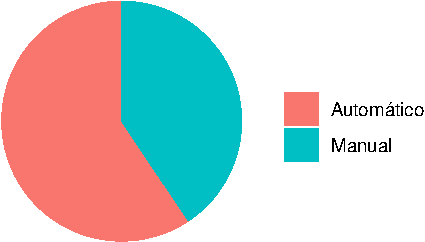
\includegraphics{inferencia_com_R_files/figure-latex/unnamed-chunk-24-1} \end{center}

Uma situação diferente ocorre quando desejamos comparar a distribuição de frequências de uma mesma variável em vários grupos, como por exemplo, a frequência de estudantes com olhos azuis entre todas as cores de cabelo na base de dados \(\texttt{HairEyeColor}\). Se quisermos usar o gráfico de setores para fazer essa comparação, devemos fazer quatro gráficos, um para cada cor de cabelo, com duas fatias cada um (olhos azuis e olhos não azuis). Uma alternativa é a construção de um gráfico de colunas (barras) como os gráficos das figuras a seguir, onde há uma barra para cada cor de cabelo representando a frequência de estudantes com olhos azuis e aquela cor de cabelo. Além de economizar espaço na apresentação, permite que as comparações sejam feitas de maneira mais rápida.

\begin{Shaded}
\begin{Highlighting}[]
\NormalTok{df }\OtherTok{=} \FunctionTok{data.frame}\NormalTok{(HairEyeColor[,,}\DecValTok{1}\NormalTok{] }\SpecialCharTok{+}\NormalTok{ HairEyeColor[,,}\DecValTok{2}\NormalTok{])}
\NormalTok{df }\OtherTok{=}\NormalTok{ df }\SpecialCharTok{\%\textgreater{}\%} \FunctionTok{filter}\NormalTok{(Eye }\SpecialCharTok{==} \StringTok{"Blue"}\NormalTok{)}
\NormalTok{p1 }\OtherTok{=}\NormalTok{ df }\SpecialCharTok{\%\textgreater{}\%} \FunctionTok{mutate}\NormalTok{(}\AttributeTok{name =} \FunctionTok{fct\_reorder}\NormalTok{(Hair, }\FunctionTok{desc}\NormalTok{(Freq))) }\SpecialCharTok{\%\textgreater{}\%}
  \FunctionTok{ggplot}\NormalTok{(}\FunctionTok{aes}\NormalTok{(}\AttributeTok{x=}\NormalTok{name, }\AttributeTok{y=}\NormalTok{Freq, }\AttributeTok{fill=}\NormalTok{name)) }\SpecialCharTok{+}
  \FunctionTok{geom\_bar}\NormalTok{(}\AttributeTok{position=}\StringTok{"dodge"}\NormalTok{, }\AttributeTok{stat=}\StringTok{"identity"}\NormalTok{) }\SpecialCharTok{+}
  \FunctionTok{geom\_text}\NormalTok{(}\FunctionTok{aes}\NormalTok{(}\AttributeTok{label =}\NormalTok{ Freq),}\AttributeTok{position=}\FunctionTok{position\_stack}\NormalTok{(}\AttributeTok{vjust =} \FloatTok{0.5}\NormalTok{)) }\SpecialCharTok{+}
  \FunctionTok{theme}\NormalTok{(}\AttributeTok{legend.position =} \StringTok{"none"}\NormalTok{,}
        \AttributeTok{axis.title.x =} \FunctionTok{element\_blank}\NormalTok{(),}
        \AttributeTok{axis.ticks.x =} \FunctionTok{element\_blank}\NormalTok{(),}
        \AttributeTok{axis.title.y =} \FunctionTok{element\_blank}\NormalTok{())}
\NormalTok{p2 }\OtherTok{=}\NormalTok{ df }\SpecialCharTok{\%\textgreater{}\%} \FunctionTok{mutate}\NormalTok{(}\AttributeTok{name =} \FunctionTok{fct\_reorder}\NormalTok{(Hair, Freq)) }\SpecialCharTok{\%\textgreater{}\%}
  \FunctionTok{ggplot}\NormalTok{(}\FunctionTok{aes}\NormalTok{(}\AttributeTok{x=}\NormalTok{name, }\AttributeTok{y=}\NormalTok{Freq, }\AttributeTok{fill=}\NormalTok{name)) }\SpecialCharTok{+}
  \FunctionTok{geom\_bar}\NormalTok{(}\AttributeTok{position=}\StringTok{"dodge"}\NormalTok{, }\AttributeTok{stat=}\StringTok{"identity"}\NormalTok{) }\SpecialCharTok{+}
  \FunctionTok{geom\_text}\NormalTok{(}\FunctionTok{aes}\NormalTok{(}\AttributeTok{label =}\NormalTok{ Freq),}\AttributeTok{position=}\FunctionTok{position\_stack}\NormalTok{(}\AttributeTok{vjust =} \FloatTok{0.5}\NormalTok{)) }\SpecialCharTok{+}
  \FunctionTok{coord\_flip}\NormalTok{() }\SpecialCharTok{+}
  \FunctionTok{theme}\NormalTok{(}\AttributeTok{legend.position =} \StringTok{"none"}\NormalTok{,}
        \AttributeTok{axis.title.x =} \FunctionTok{element\_blank}\NormalTok{(),}
        \AttributeTok{axis.ticks.x =} \FunctionTok{element\_blank}\NormalTok{(),}
        \AttributeTok{axis.title.y =} \FunctionTok{element\_blank}\NormalTok{())}
\NormalTok{gridExtra}\SpecialCharTok{::}\FunctionTok{grid.arrange}\NormalTok{(p1,p2,}\AttributeTok{ncol=}\DecValTok{2}\NormalTok{)}
\end{Highlighting}
\end{Shaded}

\begin{center}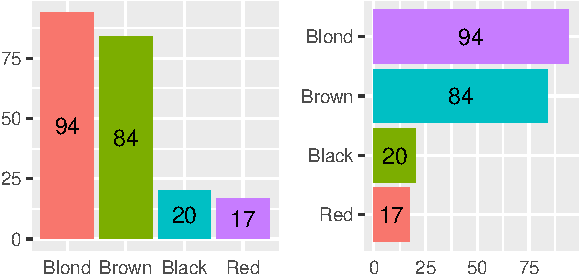
\includegraphics{inferencia_com_R_files/figure-latex/unnamed-chunk-25-1} \end{center}

A ordem dos grupos pode ser qualquer, ou aquela mais adequada para a presente análise. Frequentemente, encontramos as barras em ordem decrescente, já antecipando nossa intuição de ordenar os grupos de acordo com sua frequência para facilitar as comparações. Caso a variável fosse do tipo ordinal, a ordem das barras seria a ordem natural das categorias, como na tabela de frequências.

A figura abaixo mostra um gráfico de barras que pode ser usado da comparação da distribuição de frequências de uma mesma variável em vários grupos. É também uma alternativa ao uso de vários gráficos de setores, sendo, na verdade, a junção de dois gráficos com os das figuras acima num só gráfico. Porém, esse tipo de gráfico só deve ser usado quando não houver muitos grupos a serem comparados e a variável em estudo não tiver muitas categorias.

\begin{Shaded}
\begin{Highlighting}[]
\NormalTok{df }\OtherTok{=} \FunctionTok{data.frame}\NormalTok{(HairEyeColor[,,}\DecValTok{1}\NormalTok{] }\SpecialCharTok{+}\NormalTok{ HairEyeColor[,,}\DecValTok{2}\NormalTok{])}
\FunctionTok{ggplot}\NormalTok{(df,}\FunctionTok{aes}\NormalTok{(}\AttributeTok{x=}\NormalTok{Hair, }\AttributeTok{y=}\NormalTok{Freq, }\AttributeTok{fill=}\NormalTok{Eye)) }\SpecialCharTok{+}
  \FunctionTok{geom\_bar}\NormalTok{(}\AttributeTok{stat=}\StringTok{"identity"}\NormalTok{) }\SpecialCharTok{+}
  \FunctionTok{geom\_text}\NormalTok{(}\FunctionTok{aes}\NormalTok{(}\AttributeTok{label =}\NormalTok{ Freq),}\AttributeTok{position=}\FunctionTok{position\_stack}\NormalTok{(}\AttributeTok{vjust =} \FloatTok{0.5}\NormalTok{))}
\end{Highlighting}
\end{Shaded}

\begin{center}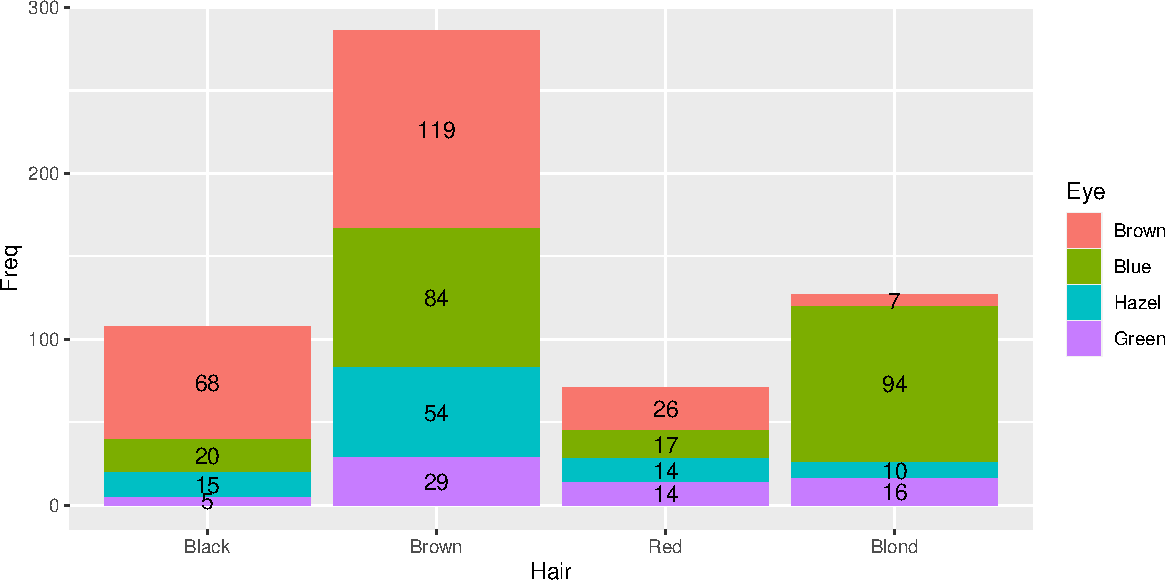
\includegraphics{inferencia_com_R_files/figure-latex/unnamed-chunk-26-1} \end{center}

Frequentemente, é necessário fazer comparações da distribuição de frequências de uma variável em vários grupos simultaneamente. Nesse caso, o uso de gráficos bem escolhidos e construídos torna a tarefa muito mais fácil. Na figura abaixo, está representada a distribuição de frequências da cor dos olhos segundo a variável cor do cabelo.

\begin{Shaded}
\begin{Highlighting}[]
\NormalTok{df }\OtherTok{=} \FunctionTok{data.frame}\NormalTok{(HairEyeColor[,,}\DecValTok{1}\NormalTok{] }\SpecialCharTok{+}\NormalTok{ HairEyeColor[,,}\DecValTok{2}\NormalTok{])}
\FunctionTok{ggplot}\NormalTok{(df,}\FunctionTok{aes}\NormalTok{(}\AttributeTok{x=}\NormalTok{Hair, }\AttributeTok{y=}\NormalTok{Freq, }\AttributeTok{fill=}\NormalTok{Eye)) }\SpecialCharTok{+}
  \FunctionTok{geom\_bar}\NormalTok{(}\AttributeTok{position=}\StringTok{"dodge"}\NormalTok{,}\AttributeTok{stat=}\StringTok{"identity"}\NormalTok{) }\SpecialCharTok{+}
  \FunctionTok{geom\_text}\NormalTok{(}\FunctionTok{aes}\NormalTok{(}\AttributeTok{label =}\NormalTok{ Freq),}\AttributeTok{position=}\FunctionTok{position\_dodge}\NormalTok{(}\AttributeTok{width =} \DecValTok{1}\NormalTok{))}
\end{Highlighting}
\end{Shaded}

\begin{center}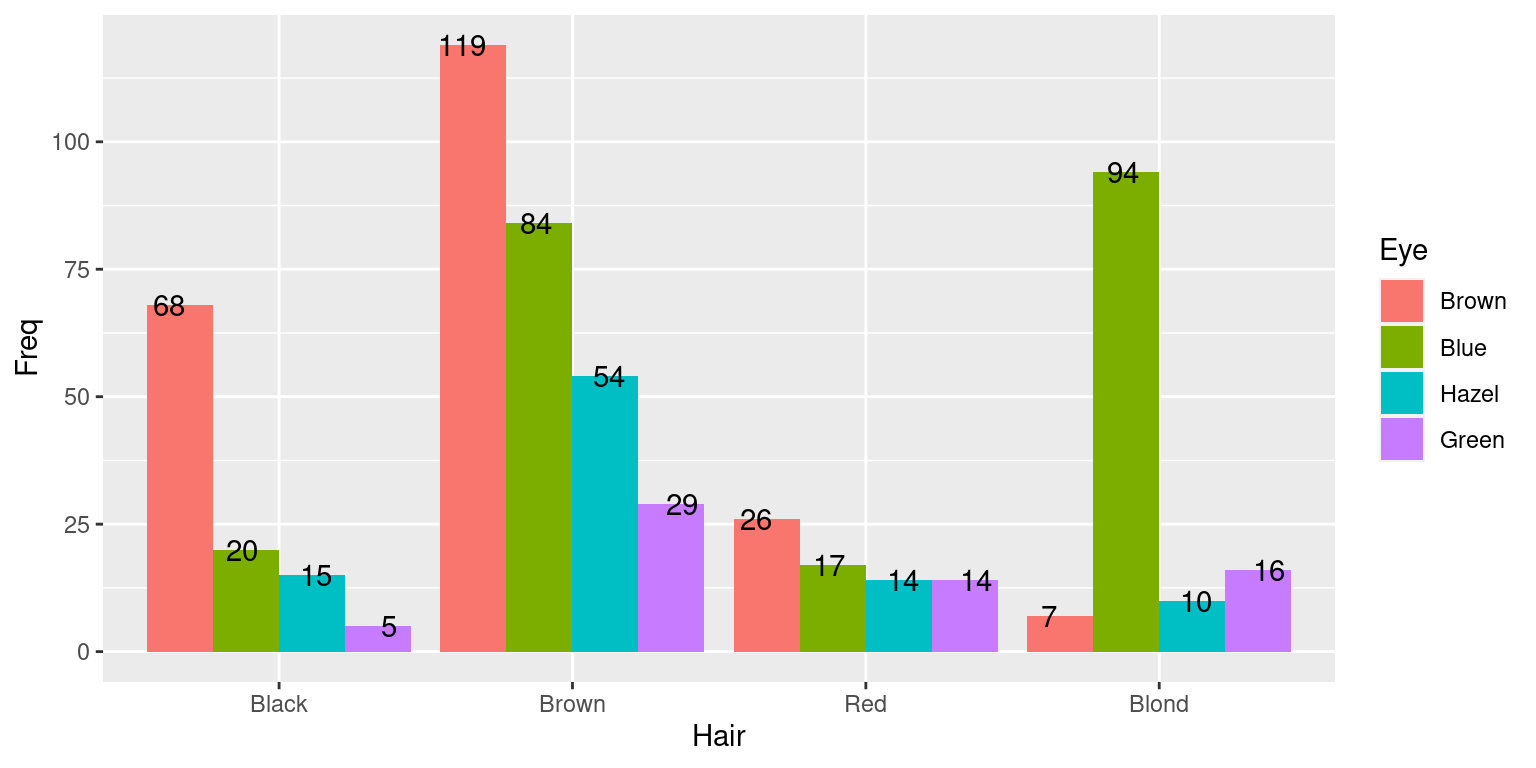
\includegraphics{inferencia_com_R_files/figure-latex/unnamed-chunk-27-1} \end{center}

\hypertarget{variuxe1veis-quantitativas-discretas}{%
\section{Variáveis Quantitativas Discretas}\label{variuxe1veis-quantitativas-discretas}}

Quando estamos trabalhando com uma variável discreta que assume poucos valores, podemos dar a ela o mesmo tratamento dado às variáveis qualitativas ordinais, assumindo que cada valor é uma classe e que existe uma ordem natural nessas classes.

Quando trabalhamos com uma variável discreta que pode assumir um grande número de valores distintos como, por exemplo, parte inteira da temperatura máxima, a construção da tabela de frequências e de gráficos considerando cada valor como uma categoria fica inviável. A solução é agrupar os valores em classes ao montar a tabela, como mostra a tabela abaixo.

\begin{tabular}{l>{\raggedleft\arraybackslash}p{2.5cm}>{\raggedleft\arraybackslash}p{2.5cm}>{\raggedright\arraybackslash}p{2.5cm}>{\raggedright\arraybackslash}p{2.5cm}}
\toprule
Temperatura & Frequência Absoluta & Frequência Relativa (\%) & Frequência Absoluta Acumulada & Frequência Relativa Acumulada (\%)\\
\midrule
56 a 67 & 21 & 15.67 & 21 & 15.67\\
67 a 78 & 47 & 35.07 & 68 & 50.75\\
78 a 89 & 66 & 49.25 & 134 & 100\\
Total & 134 & 99.99 & - & -\\
\bottomrule
\end{tabular}

A Figura abaixo mostra o gráfico da distribuição de frequências da temperatura medida por 236 dias consecutivos.

\begin{Shaded}
\begin{Highlighting}[]
\NormalTok{dt }\SpecialCharTok{\%\textgreater{}\%} \FunctionTok{filter}\NormalTok{(dt}\SpecialCharTok{$}\NormalTok{Variavel }\SpecialCharTok{!=} \StringTok{"Total"}\NormalTok{) }\SpecialCharTok{\%\textgreater{}\%} 
  \FunctionTok{ggplot}\NormalTok{(}\FunctionTok{aes}\NormalTok{(}\AttributeTok{x=}\NormalTok{Variavel, }\AttributeTok{y=}\NormalTok{Freq\_rel)) }\SpecialCharTok{+}
  \FunctionTok{geom\_bar}\NormalTok{(}\AttributeTok{position=}\StringTok{"dodge"}\NormalTok{,}\AttributeTok{stat=}\StringTok{"identity"}\NormalTok{) }\SpecialCharTok{+}
  \FunctionTok{labs}\NormalTok{(}\AttributeTok{x=}\StringTok{"Temperatura"}\NormalTok{,}\AttributeTok{y=}\StringTok{"Frequência Relativa (\%)"}\NormalTok{) }\SpecialCharTok{+}
  \FunctionTok{theme}\NormalTok{(}\AttributeTok{legend.position =} \StringTok{"none"}\NormalTok{)}
\end{Highlighting}
\end{Shaded}

\begin{center}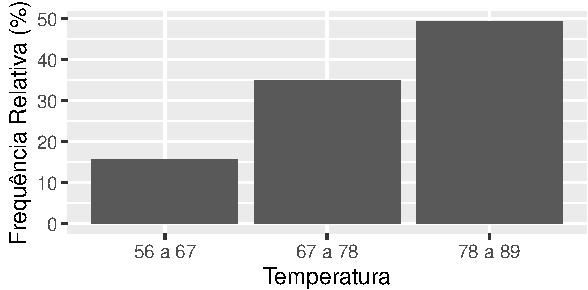
\includegraphics{inferencia_com_R_files/figure-latex/unnamed-chunk-29-1} \end{center}

\hypertarget{variuxe1veis-quantitativas-contuxednuas}{%
\section{Variáveis Quantitativas Contínuas}\label{variuxe1veis-quantitativas-contuxednuas}}

Quando a variável em estudo é do tipo contínua, que assume muitos valores distintos, o agrupamento dos dados em classes será sempre necessário na construção das tabelas de frequências. A tabela abaixo apresenta a distribuição de frequências para o peso dos carros.

\begin{tabular}{l>{\raggedleft\arraybackslash}p{2.5cm}>{\raggedleft\arraybackslash}p{2.5cm}>{\raggedright\arraybackslash}p{2.5cm}>{\raggedright\arraybackslash}p{2.5cm}}
\toprule
Temperatura & Frequência Absoluta & Frequência Relativa (\%) & Frequência Absoluta Acumulada & Frequência Relativa Acumulada (\%)\\
\midrule
1.5 |- 2 & 0 & 0.00 & 0 & 0\\
2 |- 2.5 & 0 & 0.00 & 0 & 0\\
2.5 |- 3 & 3 & 9.38 & 3 & 9.38\\
3 |- 3.5 & 10 & 31.25 & 13 & 40.62\\
3.5 |- 4 & 12 & 37.50 & 25 & 78.12\\
\addlinespace
4 |- 4.5 & 6 & 18.75 & 31 & 96.88\\
4.5 |- 5 & 1 & 3.12 & 32 & 100\\
5 |- 5.5 & 0 & 0.00 & 32 & 100\\
Total & 32 & 100.00 & - & -\\
\bottomrule
\end{tabular}

\hypertarget{histograma}{%
\section{Histograma}\label{histograma}}

A representação gráfica da distribuição de frequências de uma variável contínua é feita através de um gráfico chamado histograma, mostrado nas figuras abaixo com o peso de diamantes (\(\texttt{diamonds}\)). O histograma nada mais é do que o gráfico de barras verticais, porém construído com as barras unidas, devido ao caráter contínuo dos valores da variável.

\begin{Shaded}
\begin{Highlighting}[]
\FunctionTok{library}\NormalTok{(ggplot2)}
\NormalTok{p1}\OtherTok{=}\FunctionTok{ggplot}\NormalTok{(diamonds,}\FunctionTok{aes}\NormalTok{(carat)) }\SpecialCharTok{+}
  \FunctionTok{geom\_histogram}\NormalTok{(}\AttributeTok{color =} \StringTok{"white"}\NormalTok{) }\SpecialCharTok{+}
  \FunctionTok{labs}\NormalTok{(}\AttributeTok{y =} \StringTok{"Frequência Absoluta"}\NormalTok{)}
\NormalTok{p2}\OtherTok{=}\FunctionTok{ggplot}\NormalTok{(diamonds,}\FunctionTok{aes}\NormalTok{(carat)) }\SpecialCharTok{+}
  \FunctionTok{geom\_histogram}\NormalTok{(}\FunctionTok{aes}\NormalTok{(}\AttributeTok{y =}\NormalTok{ (..count..)}\SpecialCharTok{/}\FunctionTok{sum}\NormalTok{(..count..)}\SpecialCharTok{*}\DecValTok{100}\NormalTok{),}\AttributeTok{color =} \StringTok{"white"}\NormalTok{) }\SpecialCharTok{+}
  \FunctionTok{labs}\NormalTok{(}\AttributeTok{y =} \StringTok{"Frequência Relativa (\%)"}\NormalTok{)}
\NormalTok{gridExtra}\SpecialCharTok{::}\FunctionTok{grid.arrange}\NormalTok{(p1,p2,}\AttributeTok{ncol=}\DecValTok{2}\NormalTok{)}
\end{Highlighting}
\end{Shaded}

\begin{center}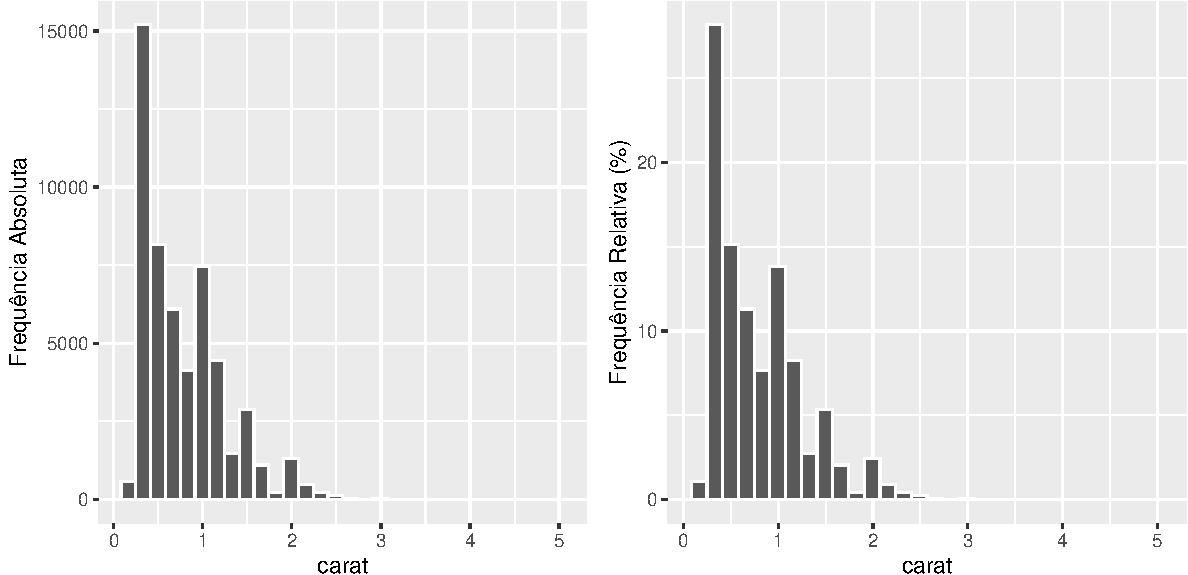
\includegraphics{inferencia_com_R_files/figure-latex/unnamed-chunk-31-1} \end{center}

Os histogramas das figuras acima têm exatamente a mesma forma, apesar de serem construídos usando as frequências absolutas e relativas, respectivamente. O objetivo dessas figuras é mostrar que a escolha do tipo de frequência a ser usada não muda a forma da distribuição. Entretanto, o uso da frequência relativa torna o histograma comparável a outros histogramas, mesmo que os conjuntos de dados tenham tamanhos diferentes (desde a mesma escala seja usada!)

Para o desenvolvimento do histograma:

\begin{itemize}
\tightlist
\item
  Calcule a amplitude dos dados
\item
  Defina a quantidade de classes (as barras verticais). Não existe uma regra, porém uma boa aproximação seria calcular a raiz quadrada da quantidade de dados (\(\sqrt n\))
\item
  Calcule o intervalo das classes dividindo a amplitude pela quantidade de classes
\item
  Determine os limites das classes. Selecione o valor mínimo dos dados (se for mais viável, ele pode ser arredondado para baixo) e soma o valor do intervalo de classe para obter o limite superior
\item
  Faça o passo anterior para todas as classes
\item
  Calcule a frequência dos dados que pertence a cada intervalo
\end{itemize}

Este é o passo a passo básico para a elaboração de um Histograma, que seja capaz de lhe trazer informações precisas sobre a frequência com que algo acontece em um determinado contexto.

Ao estudarmos a distribuição de frequências de uma variável quantitativa, seja em um grupo apenas ou comparando vários grupos, devemos verificar basicamente três características:

\begin{itemize}
\tightlist
\item
  Tendência Central;
\item
  Variabilidade;
\item
  Forma.
\end{itemize}

Tais características podem ser quantificadas através das medidas de síntese numérica ou visualizadas a partir do histograma.

\hypertarget{tenduxeancia-central}{%
\subsection{Tendência Central}\label{tenduxeancia-central}}

A tendência central da distribuição de frequências de uma variável é caracterizada pelo valor (ou faixa de valores) ``típico'' da variável.

Uma das maneiras de representar o que é ``típico'' é através do valor mais frequente da variável, chamado de moda. Ou, no caso da tabela de frequências, a classe de maior frequência, chamada de classe modal. No histograma, esta classe corresponde àquela com barra mais alta (``pico'').

\begin{center}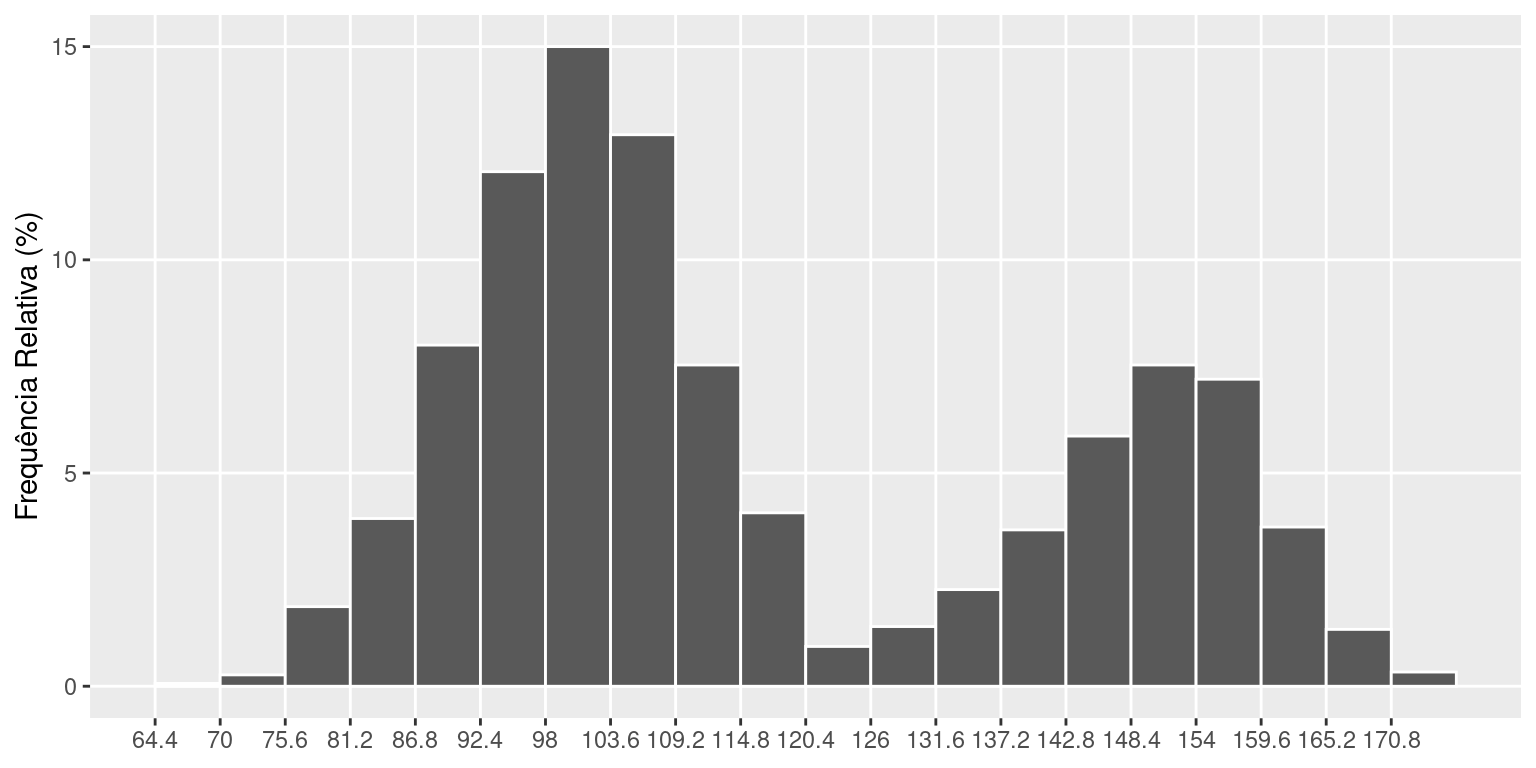
\includegraphics{inferencia_com_R_files/figure-latex/unnamed-chunk-32-1} \end{center}

No exemplo acima, a classe modal é a que vai de 92.3 até 97.9. Assim, os dados repousam, tipicamente entre esses valores. Entretanto, temos dois picos.

Geralmente, um histograma bimodal indica a existência de dois grupos, com valores centrados em dois pontos diferentes do eixo de valores. Uma distribuição de frequências pode também ser amodal, ou seja, todos os valores são igualmente frequentes. Ou também unimodal, quando os valores estão concentrados somente em um ponto/classe.

\hypertarget{variabilidade}{%
\subsection{Variabilidade}\label{variabilidade}}

Para descrever adequadamente a distribuição de frequências de uma variável quantitativa, além da informação do valor representativo da variável (tendência central), é necessário dizer também o quanto estes valores variam, ou seja, o quão dispersos eles são.

De fato, somente a informação sobre a tendência central de um conjunto de dados não consegue representá-lo adequadamente. A Figura abaixo mostra um histograma para os tempos de espera de 1000 clientes de dois bancos, um com fila única e outro com fila múltipla, com o mesmo número de atendentes. Os tempos de espera nos dois bancos têm a mesma tendência central de 7 minutos. Entretanto, os dois conjuntos de dados são claramente diferentes, pois os valores são muito mais dispersos no banco com fila múltipla. Assim, quando entramos num fila única, esperamos ser atendidos em cerca de 7 minutos, com uma variação de, no máximo, meio minuto a mais ou a menos. Na fila múltipla, a variação é maior, indicando-se que tanto pode-se esperar muito mais ou muito menos que o valor típico de 7 minutos.

\begin{center}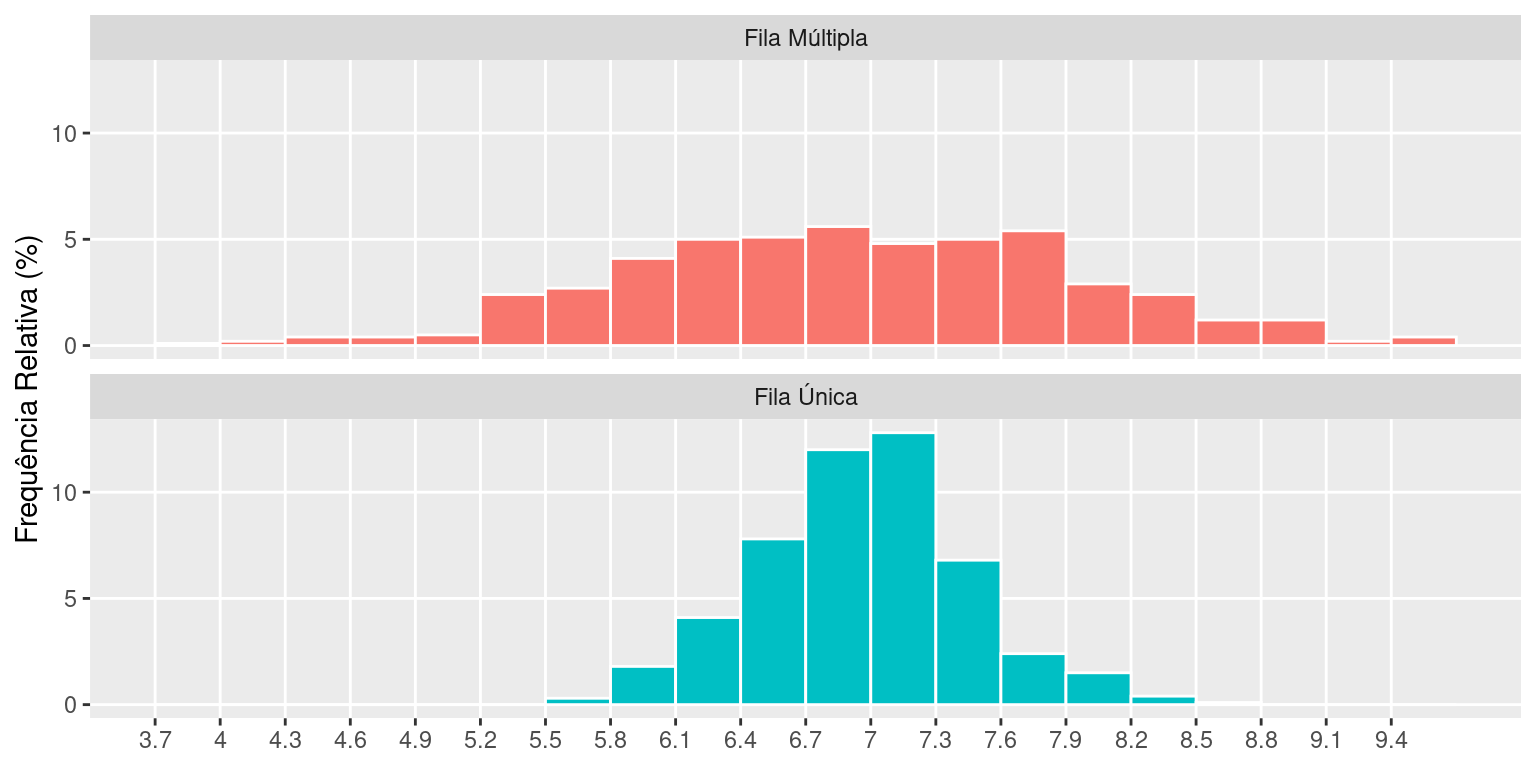
\includegraphics{inferencia_com_R_files/figure-latex/unnamed-chunk-33-1} \end{center}

\hypertarget{forma}{%
\subsection{Forma}\label{forma}}

A distribuição de frequências de uma variável pode ter várias formas, mas existem três formas básicas, apresentadas na figura abaixo através de histogramas.

\begin{center}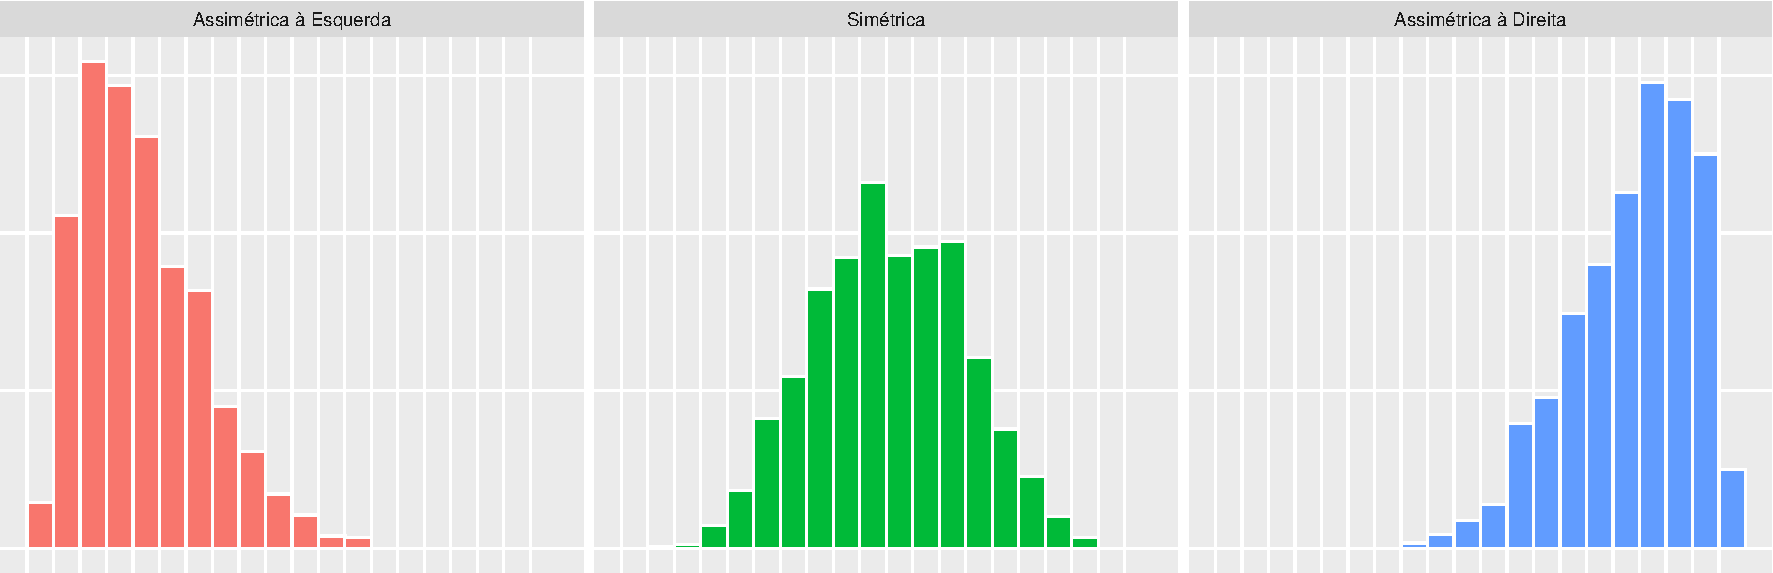
\includegraphics{inferencia_com_R_files/figure-latex/unnamed-chunk-34-1} \end{center}

Quando uma distribuição é simétrica em torno de um valor (o mais frequente), significa que as observações estão igualmente distribuídas em torno desse valor (metade acima e metade abaixo).

A assimetria de uma distribuição pode ocorrer de duas formas:

\begin{itemize}
\tightlist
\item
  quando os valores concentram-se à esquerda (assimetria com concentração à esquerda ou assimetria com cauda à direita);
\item
  quando os valores concentram-se à direita (assimetria com concentração à direita ou com assimetria cauda à esquerda);
\end{itemize}

Ao definir a assimetria de uma distribuição, algumas pessoas preferem se referir ao lado onde está a concentração dos dados. Porém, outras pessoas preferem se referir ao lado onde está ``faltando'' dados (cauda). As duas denominações são alternativas.

Em alguns casos, apenas o conhecimento da forma da distribuição de frequências de uma variável já nos fornece uma boa informação sobre o comportamento dessa variável. Por exemplo, o que você acharia se soubesse que a distribuição de frequências das notas da primeira prova da disciplina de Estatística que você está cursando é, geralmente, assimétrica com concentração à direita? Como você acha que é a forma da distribuição de frequências da renda no Brasil?

\hypertarget{boxplot}{%
\section{Boxplot}\label{boxplot}}

O Boxplot é um gráfico proposto para a detecção de valores discrepantes (outliers), que são aqueles valores muito diferentes do restante do conjunto de dados.

Esses valores discrepantes podem representar erros no processo de coleta ou de processamento dos dados, e, nesse caso, devem ser corrigidos ou excluídos do banco de dados. No entanto, os outliers podem ser valores corretos, que, por alguma razão, são muito diferentes dos demais valores. Nesse caso, a análise desses dados deve ser cuidadosa, pois, como sabemos, algumas estatísticas descritivas, como a média e o desvio-padrão, são influenciadas por valores extremos.

Na construção do Boxplot, utilizamos alguns percentis (mediana, primeiro e terceiro quartis), que são pouco influenciados por valores extremos. Além disso, precisamos saber quais são os valores mínimo e máximo do conjunto de dados.

O Boxplot é constituído por uma caixa atravessada por uma linha, construído usando um eixo com uma escala de valores, como mostra a figura abaixo. Como sabemos, entre o primeiro e o terceiro quartis, temos 50\% dos dados. Podemos pensar, então, que essa caixa contém metade dos dados do conjunto.

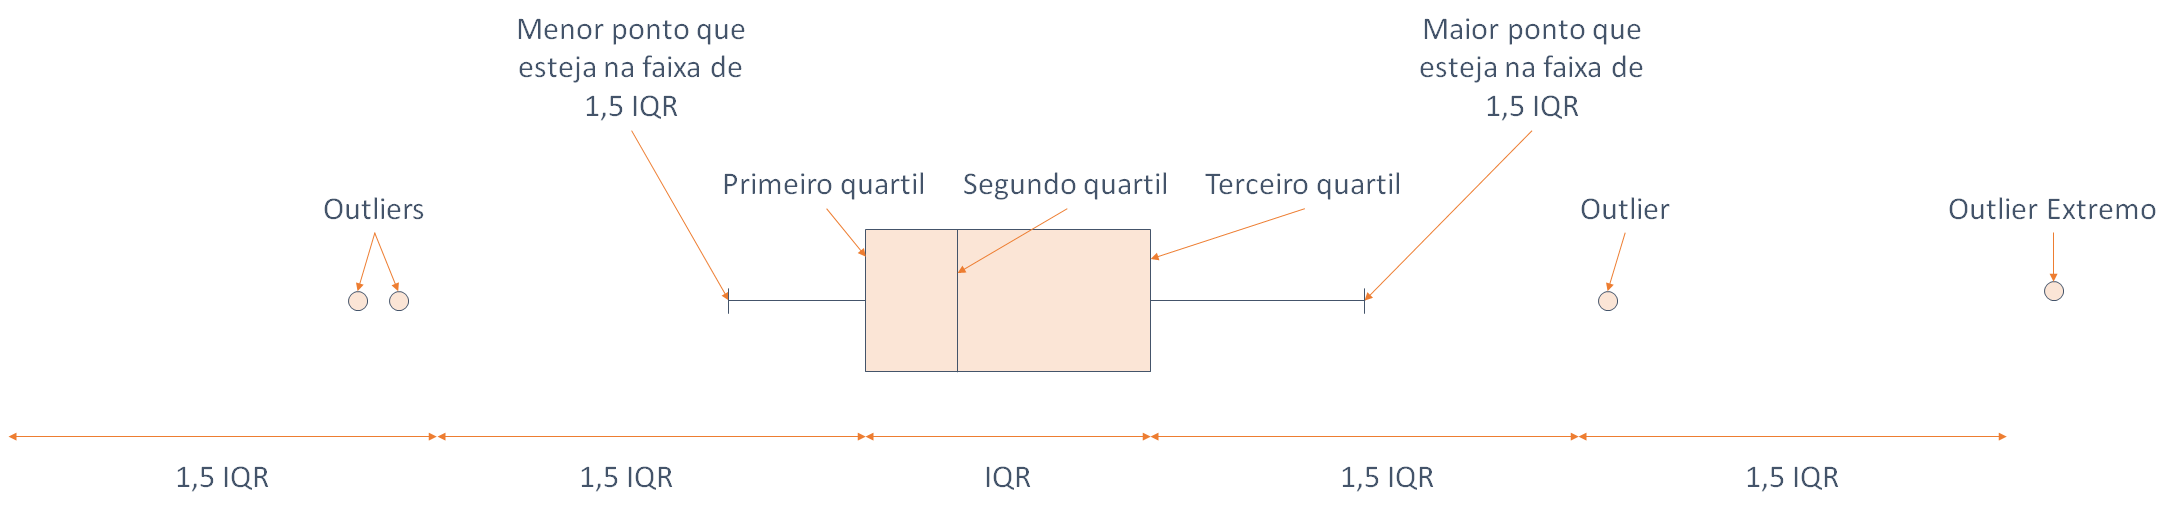
\includegraphics{Boxplot exemplo.png}

Como um gráfico tem que representar todos os valores do conjunto de dados, precisamos representar os outros 50\%, sendo 25\% abaixo do Q1 e 25\% acima do Q3. Esses valores serão representados pelas duas linhas que saem das extremidades da caixa. Cada uma das linhas é traçada, a partir das extremidades da caixa, até que encontre o valor máximo ou mínimo; ou atinja o comprimento máximo de 1,5 vezes a altura da caixa (IQR). O que acontecer primeiro.

No exemplo da imagem acima o segundo caso aconteceu, assim os valores que ainda não foram representados devem ser devidamente marcados em suas respectivas posições na escala de valores. Esses valores são considerados outliers pelo critério do boxplot. Obviamente, o limite superior do boxplot não coincidiu com o valor máximo do conjunto de dados, que foi considerado um valor discrepante (outlier).

Além da detecção de valores discrepantes, o boxplot pode ser muito útil na análise da distribuição dos valores de um conjunto de dados. Através do boxplot, podemos:

\begin{itemize}
\tightlist
\item
  identificar a forma da distribuição (simétrica ou assimétrica);
\item
  avaliar e comparar a tendência central (mediana) de dois ou mais conjuntos de dados;
\item
  comparar a variabilidade de dois ou mais conjuntos de dados
\end{itemize}

Para avaliar a forma da distribuição, devemos observar o deslocamento da caixa em relação a linha do boxplot. Lembrando que a caixa do boxplot contém 50\% dos dados, o seu deslocamento na linha nos informa onde estão concentrados os dados.

Se a caixa está mais deslocada para um dos lados da linha, significa que metade dos dados estão concentrados naquele lado da escala de valores e, assim, a distribuição é assimétrica. Se a caixa está praticamente no meio da linha, dividindo-a em duas partes iguais, é distribuição será considerada simétrica.

\begin{center}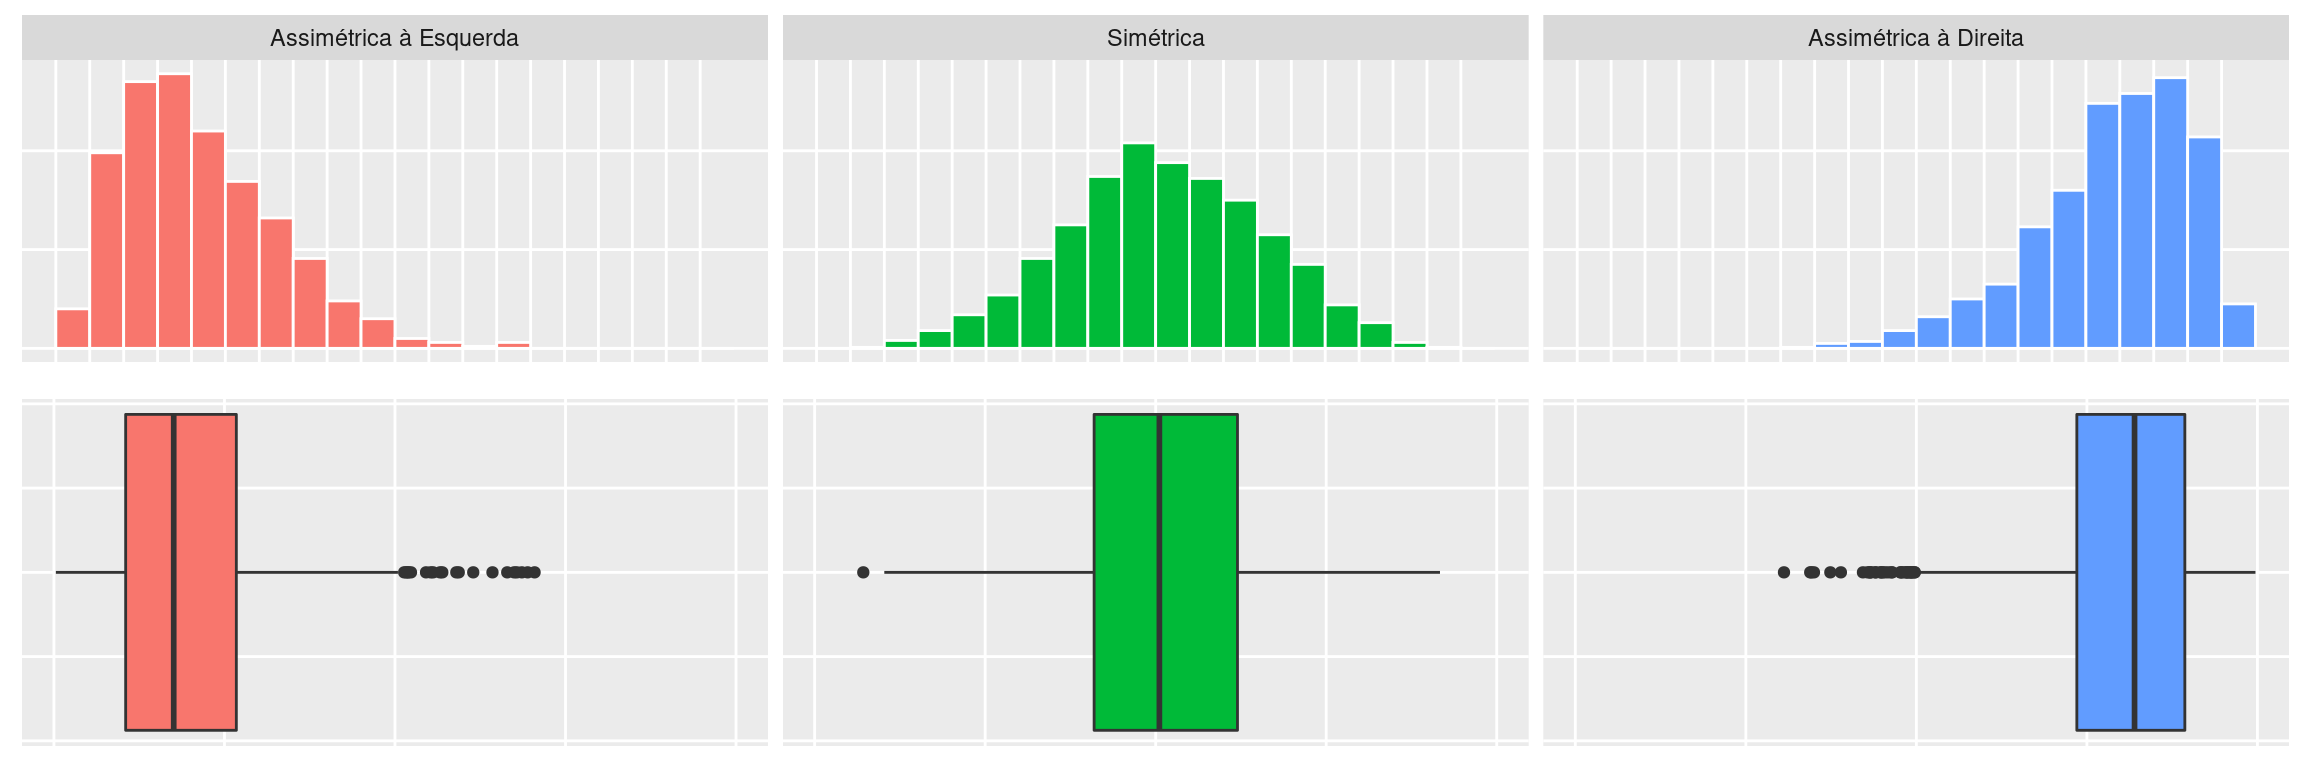
\includegraphics{inferencia_com_R_files/figure-latex/unnamed-chunk-36-1} \end{center}

\hypertarget{diagrama-de-dispersuxe3o}{%
\section{Diagrama de Dispersão}\label{diagrama-de-dispersuxe3o}}

O diagrama de dispersão é um gráfico onde pontos no espaço cartesiano XY são usados para representar simultaneamente os valores de duas variáveis quantitativas medidas em cada indivíduo do conjunto de dados.

O Quadro e a Figura abaixo mostram um esquema do desenho do diagrama de dispersão. Neste exemplo, foram medidos os valores de duas variáveis quantitativas, X e Y, em quatro indivíduos. O eixo horizontal do gráfico representa a variável X e o eixo vertical representa a variável Y.

\begin{tabular}{l>{\raggedleft\arraybackslash}p{2.5cm}>{\raggedleft\arraybackslash}p{2.5cm}>{}p{2.5cm}>{}p{2.5cm}}
\toprule
Indivíduos & Variável X & Variável Y\\
\midrule
A & 2 & 3\\
B & 4 & 3\\
C & 4 & 5\\
D & 8 & 7\\
\bottomrule
\end{tabular}

\begin{center}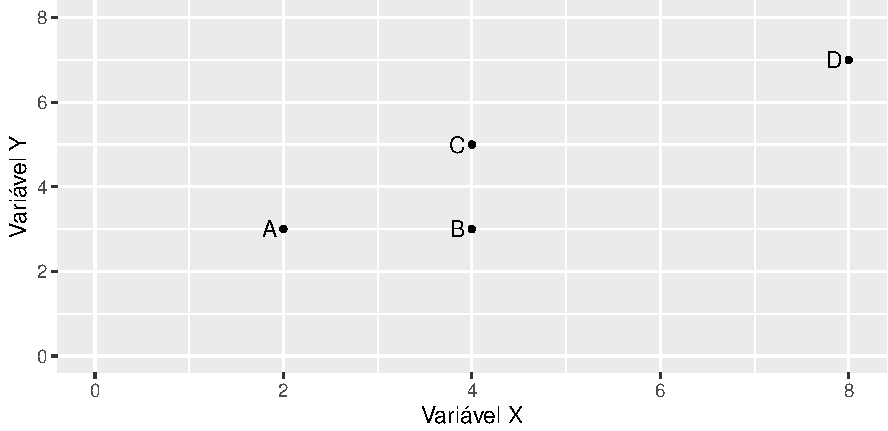
\includegraphics{inferencia_com_R_files/figure-latex/unnamed-chunk-37-1} \end{center}

O diagrama de dispersão é usado principalmente para visualizar a relação/associação entre duas variáveis, mas também para é muito útil para:

\begin{itemize}
\tightlist
\item
  Comparar o efeito de dois tratamentos no mesmo indivíduo
\item
  Verificar o efeito tipo antes/depois de um tratamento
\end{itemize}

A seguir, veremos dois exemplos da utilização do diagrama de dispersão. O primeiro refere-se ao estudo da associação entre duas variáveis. O segundo utiliza o diagrama de dispersão para comparar o efeito da aplicação de um tratamento, comparando as medidas antes e depois da medicação.

\hypertarget{exemplo-1}{%
\subsection{Exemplo 1}\label{exemplo-1}}

Um produtor de morangos para exportação deseja produzir frutos grandes, pois frutos pequenos têm pouco valor mesmo no mercado interno. Além disso, os frutos, mesmo grandes, não devem ter tamanhos muito diferentes entre si. O produtor suspeita que uma dos fatores que altera o tamanho dos frutos é o número de frutos por árvore.

Para investigar a relação entre o número de frutos que uma planta produz e o peso destes frutos, ele observou dados de 10 morangueiros na primeira safra (Quadro abaixo) e gerou o Diagrama de Dispersão apresentado abaixo.

\begin{table}
\centering\begingroup\fontsize{5}{7}\selectfont

\begin{tabular}{>{\raggedleft\arraybackslash}p{0.7cm}>{\raggedleft\arraybackslash}p{0.7cm}>{\raggedleft\arraybackslash}p{0.7cm}>{\raggedleft\arraybackslash}p{0.7cm}>{\raggedleft\arraybackslash}p{0.7cm}>{\raggedleft\arraybackslash}p{0.7cm}>{\raggedleft\arraybackslash}p{0.7cm}>{\raggedleft\arraybackslash}p{0.7cm}>{\raggedleft\arraybackslash}p{0.7cm}>{\raggedleft\arraybackslash}p{0.7cm}>{\raggedleft\arraybackslash}p{0.7cm}>{\raggedleft\arraybackslash}p{0.7cm}>{\raggedleft\arraybackslash}p{0.7cm}>{\raggedleft\arraybackslash}p{0.7cm}>{\raggedleft\arraybackslash}p{0.7cm}>{\raggedleft\arraybackslash}p{0.7cm}}
\toprule
Planta & Quantidade &  &  &  &  &  &  &  &  &  &  &  &  &  & \\
\midrule
1001 & 5 & 15.15 & 15.45 & 15.63 & 15.65 & 16.38 & NA & NA & NA & NA & NA & NA & NA & NA & NA\\
1002 & 6 & 14.00 & 14.50 & 15.35 & 15.86 & 15.94 & 16.13 & NA & NA & NA & NA & NA & NA & NA & NA\\
1003 & 7 & 13.67 & 13.76 & 14.06 & 14.11 & 14.54 & 14.89 & 15.50 & NA & NA & NA & NA & NA & NA & NA\\
1004 & 8 & 11.00 & 11.50 & 12.39 & 12.39 & 12.90 & 14.50 & 15.50 & 16.56 & NA & NA & NA & NA & NA & NA\\
1005 & 9 & 10.24 & 11.12 & 12.05 & 12.37 & 13.48 & 13.80 & 14.04 & 15.39 & 16.00 & NA & NA & NA & NA & NA\\
\addlinespace
1006 & 10 & 9.00 & 9.32 & 10.67 & 11.56 & 11.67 & 12.56 & 12.83 & 12.84 & 13.43 & 15.09 & NA & NA & NA & NA\\
1007 & 11 & 7.82 & 8.56 & 8.74 & 9.57 & 11.08 & 11.92 & 12.13 & 12.50 & 14.14 & 14.20 & 14.00 & NA & NA & NA\\
1008 & 12 & 7.25 & 9.41 & 10.15 & 10.33 & 10.80 & 10.95 & 11.13 & 11.48 & 11.49 & 12.86 & 13.37 & 15.04 & NA & NA\\
1009 & 13 & 6.95 & 7.61 & 8.53 & 10.00 & 10.94 & 11.04 & 11.43 & 11.63 & 11.97 & 12.02 & 12.74 & 13.53 & 14.00 & NA\\
1010 & 14 & 7.00 & 8.00 & 9.00 & 10.00 & 10.00 & 10.50 & 11.00 & 11.16 & 11.17 & 11.70 & 12.45 & 12.89 & 13.47 & 13.54\\
\bottomrule
\end{tabular}
\endgroup{}
\end{table}

\begin{Shaded}
\begin{Highlighting}[]
\FunctionTok{library}\NormalTok{(ggplot2)}
\FunctionTok{library}\NormalTok{(tidyr)}
\NormalTok{aux }\OtherTok{=} \FunctionTok{matrix}\NormalTok{(}\FunctionTok{c}\NormalTok{(}\FloatTok{15.15}\NormalTok{,}\FloatTok{15.45}\NormalTok{,}\FloatTok{15.63}\NormalTok{,}\FloatTok{15.65}\NormalTok{,}\FloatTok{16.38}\NormalTok{,}\ConstantTok{NA}\NormalTok{,}\ConstantTok{NA}\NormalTok{,}\ConstantTok{NA}\NormalTok{,}\ConstantTok{NA}\NormalTok{,}\ConstantTok{NA}\NormalTok{,}\ConstantTok{NA}\NormalTok{,}\ConstantTok{NA}\NormalTok{,}\ConstantTok{NA}\NormalTok{,}\ConstantTok{NA}\NormalTok{,}
               \DecValTok{14}\NormalTok{,}\FloatTok{14.5}\NormalTok{,}\FloatTok{15.35}\NormalTok{,}\FloatTok{15.86}\NormalTok{,}\FloatTok{15.94}\NormalTok{,}\FloatTok{16.13}\NormalTok{,}\ConstantTok{NA}\NormalTok{,}\ConstantTok{NA}\NormalTok{,}\ConstantTok{NA}\NormalTok{,}\ConstantTok{NA}\NormalTok{,}\ConstantTok{NA}\NormalTok{,}\ConstantTok{NA}\NormalTok{,}\ConstantTok{NA}\NormalTok{,}\ConstantTok{NA}\NormalTok{,}
               \FloatTok{13.67}\NormalTok{,}\FloatTok{13.76}\NormalTok{,}\FloatTok{14.06}\NormalTok{,}\FloatTok{14.11}\NormalTok{,}\FloatTok{14.54}\NormalTok{,}\FloatTok{14.89}\NormalTok{,}\FloatTok{15.5}\NormalTok{,}\ConstantTok{NA}\NormalTok{,}\ConstantTok{NA}\NormalTok{,}\ConstantTok{NA}\NormalTok{,}\ConstantTok{NA}\NormalTok{,}\ConstantTok{NA}\NormalTok{,}\ConstantTok{NA}\NormalTok{,}\ConstantTok{NA}\NormalTok{,}
               \DecValTok{11}\NormalTok{,}\FloatTok{11.5}\NormalTok{,}\FloatTok{12.39}\NormalTok{,}\FloatTok{12.39}\NormalTok{,}\FloatTok{12.9}\NormalTok{,}\FloatTok{14.5}\NormalTok{,}\FloatTok{15.5}\NormalTok{,}\FloatTok{16.56}\NormalTok{,}\ConstantTok{NA}\NormalTok{,}\ConstantTok{NA}\NormalTok{,}\ConstantTok{NA}\NormalTok{,}\ConstantTok{NA}\NormalTok{,}\ConstantTok{NA}\NormalTok{,}\ConstantTok{NA}\NormalTok{,}
               \FloatTok{10.24}\NormalTok{,}\FloatTok{11.12}\NormalTok{,}\FloatTok{12.05}\NormalTok{,}\FloatTok{12.37}\NormalTok{,}\FloatTok{13.48}\NormalTok{,}\FloatTok{13.8}\NormalTok{,}\FloatTok{14.04}\NormalTok{,}\FloatTok{15.39}\NormalTok{,}\DecValTok{16}\NormalTok{,}\ConstantTok{NA}\NormalTok{,}\ConstantTok{NA}\NormalTok{,}\ConstantTok{NA}\NormalTok{,}\ConstantTok{NA}\NormalTok{,}\ConstantTok{NA}\NormalTok{,}
               \DecValTok{9}\NormalTok{,}\FloatTok{9.32}\NormalTok{,}\FloatTok{10.67}\NormalTok{,}\FloatTok{11.56}\NormalTok{,}\FloatTok{11.67}\NormalTok{,}\FloatTok{12.56}\NormalTok{,}\FloatTok{12.83}\NormalTok{,}\FloatTok{12.84}\NormalTok{,}\FloatTok{13.43}\NormalTok{,}\FloatTok{15.09}\NormalTok{,}\ConstantTok{NA}\NormalTok{,}\ConstantTok{NA}\NormalTok{,}\ConstantTok{NA}\NormalTok{,}\ConstantTok{NA}\NormalTok{,}
               \FloatTok{7.82}\NormalTok{,}\FloatTok{8.56}\NormalTok{,}\FloatTok{8.74}\NormalTok{,}\FloatTok{9.57}\NormalTok{,}\FloatTok{11.08}\NormalTok{,}\FloatTok{11.92}\NormalTok{,}\FloatTok{12.13}\NormalTok{,}\FloatTok{12.5}\NormalTok{,}\FloatTok{14.14}\NormalTok{,}\FloatTok{14.2}\NormalTok{,}\DecValTok{14}\NormalTok{,}\ConstantTok{NA}\NormalTok{,}\ConstantTok{NA}\NormalTok{,}\ConstantTok{NA}\NormalTok{,}
               \FloatTok{7.25}\NormalTok{,}\FloatTok{9.41}\NormalTok{,}\FloatTok{10.15}\NormalTok{,}\FloatTok{10.33}\NormalTok{,}\FloatTok{10.8}\NormalTok{,}\FloatTok{10.95}\NormalTok{,}\FloatTok{11.13}\NormalTok{,}\FloatTok{11.48}\NormalTok{,}\FloatTok{11.49}\NormalTok{,}\FloatTok{12.86}\NormalTok{,}\FloatTok{13.37}\NormalTok{,}\FloatTok{15.04}\NormalTok{,}\ConstantTok{NA}\NormalTok{,}\ConstantTok{NA}\NormalTok{,}
               \FloatTok{6.95}\NormalTok{,}\FloatTok{7.61}\NormalTok{,}\FloatTok{8.53}\NormalTok{,}\DecValTok{10}\NormalTok{,}\FloatTok{10.94}\NormalTok{,}\FloatTok{11.04}\NormalTok{,}\FloatTok{11.43}\NormalTok{,}\FloatTok{11.63}\NormalTok{,}\FloatTok{11.97}\NormalTok{,}\FloatTok{12.02}\NormalTok{,}\FloatTok{12.74}\NormalTok{,}\FloatTok{13.53}\NormalTok{,}\DecValTok{14}\NormalTok{,}\ConstantTok{NA}\NormalTok{,}
               \DecValTok{7}\NormalTok{,}\DecValTok{8}\NormalTok{,}\DecValTok{9}\NormalTok{,}\DecValTok{10}\NormalTok{,}\DecValTok{10}\NormalTok{,}\FloatTok{10.5}\NormalTok{,}\DecValTok{11}\NormalTok{,}\FloatTok{11.16}\NormalTok{,}\FloatTok{11.17}\NormalTok{,}\FloatTok{11.7}\NormalTok{,}\FloatTok{12.45}\NormalTok{,}\FloatTok{12.89}\NormalTok{,}\FloatTok{13.47}\NormalTok{,}\FloatTok{13.54}\NormalTok{),}
             \AttributeTok{nrow=}\DecValTok{10}\NormalTok{,}\AttributeTok{ncol =} \DecValTok{14}\NormalTok{,}\AttributeTok{byrow =}\NormalTok{ T)}
\NormalTok{dados }\OtherTok{=} \FunctionTok{data.frame}\NormalTok{(}\AttributeTok{ID\_Morangueiro =} \DecValTok{1001}\SpecialCharTok{:}\DecValTok{1010}\NormalTok{,}
                   \AttributeTok{Qtd\_Frutos =} \DecValTok{5}\SpecialCharTok{:}\DecValTok{14}\NormalTok{,aux)}
\NormalTok{dados }\SpecialCharTok{\%\textgreater{}\%} 
  \FunctionTok{pivot\_longer}\NormalTok{(}\FunctionTok{starts\_with}\NormalTok{(}\StringTok{"X"}\NormalTok{)) }\SpecialCharTok{\%\textgreater{}\%} 
  \FunctionTok{ggplot}\NormalTok{(}\FunctionTok{aes}\NormalTok{(}\AttributeTok{x =}\NormalTok{ Qtd\_Frutos, }\AttributeTok{y =}\NormalTok{ value)) }\SpecialCharTok{+}
  \FunctionTok{geom\_point}\NormalTok{(}\AttributeTok{size =} \DecValTok{1}\NormalTok{) }\SpecialCharTok{+}
  \FunctionTok{scale\_x\_discrete}\NormalTok{(}\AttributeTok{limits=}\DecValTok{5}\SpecialCharTok{:}\DecValTok{14}\NormalTok{) }\SpecialCharTok{+}
  \FunctionTok{labs}\NormalTok{(}\AttributeTok{x =} \StringTok{"Quantidade de Frutos"}\NormalTok{,}\AttributeTok{y =} \StringTok{"Peso do Fruto (g)"}\NormalTok{)}
\end{Highlighting}
\end{Shaded}

\begin{center}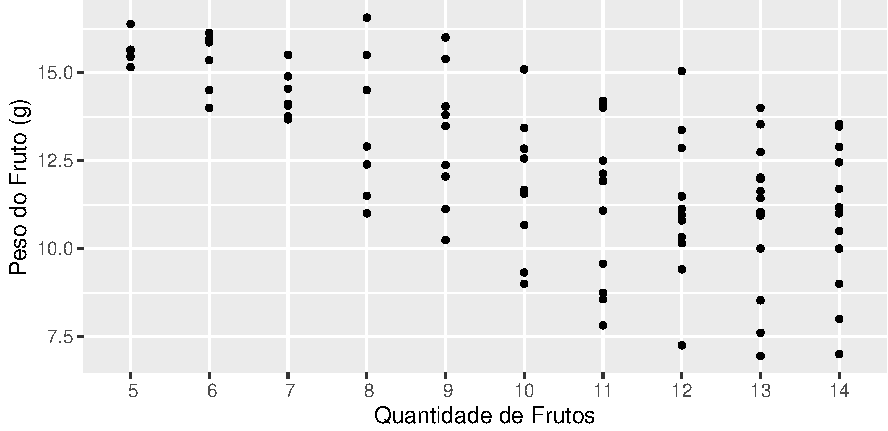
\includegraphics{inferencia_com_R_files/figure-latex/unnamed-chunk-40-1} \end{center}

O diagrama de dispersão mostra-nos dois fatos. O primeiro, que há um decréscimo no valor médio do peso do fruto por árvore à medida que cresce o número de frutos na árvore. Ou seja, não é vantagem uma árvore produzir muitos frutos, pois eles tenderão a ser muito pequenos.

O segundo fato que percebemos é que, com o aumento no número de frutos na árvore, cresce também a variabilidade no peso, gerando tanto frutos muito grandes, como muito pequenos.

Assim, conclui-se que não é vantagem ter poucas plantas produzindo muito frutos, mas sim muitas plantas produzindo poucos frutos, mas grandes e uniformes. Uma análise mais detalhada poderá determinar o número ideal de frutos por árvore, aquele que maximiza o peso médio e, ao mesmo tempo, minimiza a variabilidade do peso.

\hypertarget{exemplo-2}{%
\subsection{Exemplo 2}\label{exemplo-2}}

Captopril é um remédio destinado a baixar a pressão sistólica. Para testar seu efeito, ele foi ministrado a 12 pacientes, tendo sido medida a pressão sistólica antes e depois da medicação.

\begin{tabular}{l>{\raggedleft\arraybackslash}p{2.5cm}>{\raggedleft\arraybackslash}p{2.5cm}>{}p{2.5cm}>{}p{2.5cm}}
\toprule
Paciente & Antes & Depois\\
\midrule
A & 200 & 191\\
B & 174 & 170\\
C & 198 & 177\\
D & 170 & 167\\
E & 179 & 159\\
\addlinespace
F & 182 & 151\\
G & 193 & 176\\
H & 209 & 183\\
I & 185 & 159\\
J & 155 & 145\\
\addlinespace
K & 169 & 146\\
L & 210 & 177\\
\bottomrule
\end{tabular}

Os mesmos indivíduos foram utilizados nas duas amostras (Antes/depois). Assim, é natural compararmos a pressão sistólica para cada indivíduo, comparando a pressão sistólica depois e antes. Para todos os pacientes, a pressão sistólica depois do Captopril é menor do que antes da medicação. Mas como podemos ``ver'' se estas diferenças são grandes? Com a ajuda do diagrama de dispersão mostrado na figura abaixo.

\begin{Shaded}
\begin{Highlighting}[]
\NormalTok{dados }\OtherTok{=} \FunctionTok{data.frame}\NormalTok{(}\AttributeTok{Paciente =}\NormalTok{ LETTERS[}\DecValTok{1}\SpecialCharTok{:}\DecValTok{12}\NormalTok{],}
                   \AttributeTok{Antes =} \FunctionTok{c}\NormalTok{(}\DecValTok{200}\NormalTok{, }\DecValTok{174}\NormalTok{, }\DecValTok{198}\NormalTok{, }\DecValTok{170}\NormalTok{, }\DecValTok{179}\NormalTok{, }\DecValTok{182}\NormalTok{, }\DecValTok{193}\NormalTok{, }\DecValTok{209}\NormalTok{, }\DecValTok{185}\NormalTok{, }\DecValTok{155}\NormalTok{, }\DecValTok{169}\NormalTok{, }\DecValTok{210}\NormalTok{),}
                   \AttributeTok{Depois =} \FunctionTok{c}\NormalTok{(}\DecValTok{191}\NormalTok{, }\DecValTok{170}\NormalTok{, }\DecValTok{177}\NormalTok{, }\DecValTok{167}\NormalTok{, }\DecValTok{159}\NormalTok{, }\DecValTok{151}\NormalTok{, }\DecValTok{176}\NormalTok{, }\DecValTok{183}\NormalTok{, }\DecValTok{159}\NormalTok{, }\DecValTok{145}\NormalTok{, }\DecValTok{146}\NormalTok{, }\DecValTok{177}\NormalTok{))}

\NormalTok{dados }\SpecialCharTok{\%\textgreater{}\%}
  \FunctionTok{ggplot}\NormalTok{(}\FunctionTok{aes}\NormalTok{(}\AttributeTok{x =}\NormalTok{ Antes, }\AttributeTok{y =}\NormalTok{ Depois)) }\SpecialCharTok{+}
  \FunctionTok{geom\_point}\NormalTok{(}\AttributeTok{size =} \DecValTok{1}\NormalTok{) }\SpecialCharTok{+}
  \FunctionTok{ylim}\NormalTok{(}\DecValTok{140}\NormalTok{,}\DecValTok{220}\NormalTok{) }\SpecialCharTok{+} \FunctionTok{xlim}\NormalTok{(}\DecValTok{140}\NormalTok{,}\DecValTok{220}\NormalTok{) }\SpecialCharTok{+}
  \FunctionTok{geom\_abline}\NormalTok{(}\AttributeTok{slope =} \DecValTok{1}\NormalTok{, }\AttributeTok{intercept =} \DecValTok{0}\NormalTok{) }\SpecialCharTok{+}
  \FunctionTok{geom\_text}\NormalTok{(}\FunctionTok{aes}\NormalTok{(}\AttributeTok{x =} \DecValTok{200}\NormalTok{, }\AttributeTok{y =} \DecValTok{160}\NormalTok{), }\AttributeTok{label =} \StringTok{"Depois \textless{} Antes"}\NormalTok{) }\SpecialCharTok{+}
  \FunctionTok{geom\_text}\NormalTok{(}\FunctionTok{aes}\NormalTok{(}\AttributeTok{x =} \DecValTok{160}\NormalTok{, }\AttributeTok{y =} \DecValTok{200}\NormalTok{), }\AttributeTok{label =} \StringTok{"Depois \textgreater{} Antes"}\NormalTok{) }\SpecialCharTok{+}
  \FunctionTok{geom\_text}\NormalTok{(}\FunctionTok{aes}\NormalTok{(}\AttributeTok{x =} \DecValTok{210}\NormalTok{, }\AttributeTok{y =} \DecValTok{210}\NormalTok{), }\AttributeTok{label =} \StringTok{"Depois = Antes"}\NormalTok{)}
\end{Highlighting}
\end{Shaded}

\begin{center}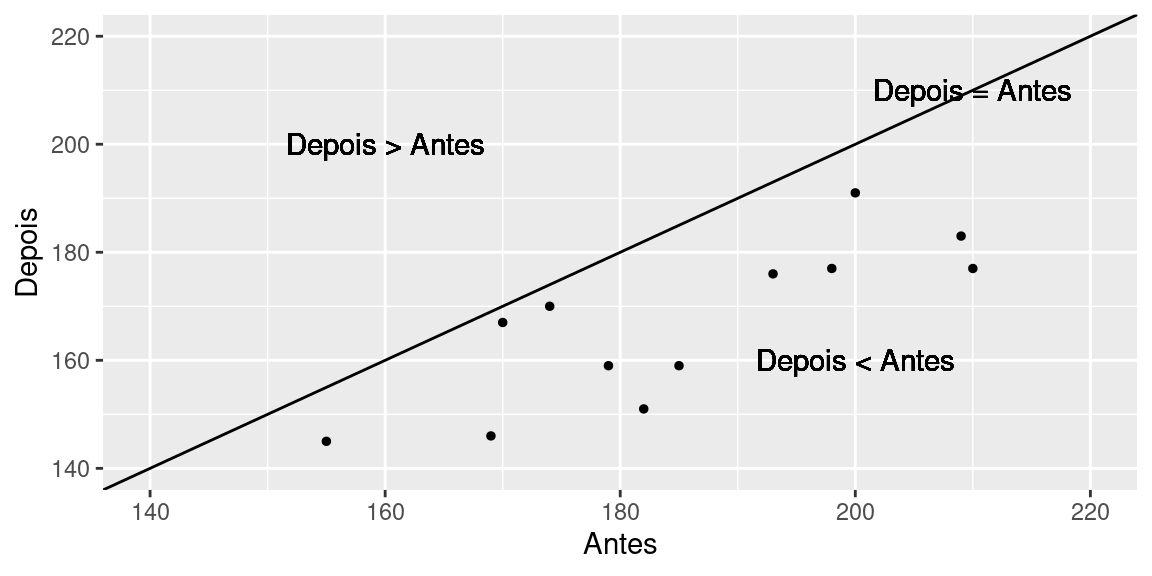
\includegraphics{inferencia_com_R_files/figure-latex/unnamed-chunk-42-1} \end{center}

Cada ponto no diagrama de dispersão corresponde às medidas de pressão sistólica de um paciente, medida antes e depois da medicação. A linha marcada no diagrama corresponde à situação onde a pressão sistólica não se alterou depois do paciente tomar o Captopril. Veja que todos os pontos estão abaixo desta linha, ou seja para todos os pacientes o Captopril fez efeito. Grande parte destes pontos está bem distante da linha, mostrando que a redução na pressão sistólica depois do uso do medicamento não foi pequena.

\hypertarget{suxe9ries-temporais}{%
\section{Séries Temporais}\label{suxe9ries-temporais}}

Séries temporais (ou séries históricas) são um conjunto de observações de uma mesma variável quantitativa (discreta ou contínua) feitas ao longo do tempo. O conjunto de novos casos da COVID-19 é um exemplo de série temporal.

Um dos objetivos do estudo de séries temporais é conhecer o comportamento da série ao longo do tempo (aumento, estabilidade ou declínio dos valores). Em alguns estudos, esse conhecimento pode ser usado para se fazer previsões de valores futuros com base no comportamento dos valores passados.

A representação gráfica de uma série temporal é feita através do gráfico de linha, como exemplificado nas figuras abaixo. No eixo horizontal do gráfico de linha, está o indicador de tempo e, no eixo vertical, a variável a ser representada.

\begin{Shaded}
\begin{Highlighting}[]
\FunctionTok{library}\NormalTok{(tsibble)}
\FunctionTok{library}\NormalTok{(lubridate)}
\FunctionTok{library}\NormalTok{(dplyr)}

\NormalTok{dados }\OtherTok{=} \FunctionTok{read.csv}\NormalTok{(}\StringTok{"https://raw.githubusercontent.com/wcota/covid19br/master/cases{-}brazil{-}states.csv"}\NormalTok{)}

\NormalTok{dados }\SpecialCharTok{\%\textgreater{}\%}
  \FunctionTok{mutate}\NormalTok{(}\AttributeTok{date =} \FunctionTok{as\_date}\NormalTok{(date)) }\SpecialCharTok{\%\textgreater{}\%} 
  \FunctionTok{as\_tsibble}\NormalTok{(}\AttributeTok{key =}\NormalTok{ state, }\AttributeTok{index =}\NormalTok{ date) }\SpecialCharTok{\%\textgreater{}\%} 
  \FunctionTok{filter}\NormalTok{(state }\SpecialCharTok{==} \StringTok{"TOTAL"}\NormalTok{) }\SpecialCharTok{\%\textgreater{}\%} 
  \FunctionTok{select}\NormalTok{(date, newCases) }\SpecialCharTok{\%\textgreater{}\%}
  \FunctionTok{ggplot}\NormalTok{(}\FunctionTok{aes}\NormalTok{(}\AttributeTok{x =}\NormalTok{ date, }\AttributeTok{y =}\NormalTok{ newCases)) }\SpecialCharTok{+}
  \FunctionTok{geom\_line}\NormalTok{() }\SpecialCharTok{+}
  \FunctionTok{labs}\NormalTok{(}\AttributeTok{title =} \StringTok{"Evolução dos casos de COVID{-}19 no Brasil"}\NormalTok{,}
       \AttributeTok{y =} \StringTok{"Novos Casos"}\NormalTok{, }\AttributeTok{x =} \StringTok{"Data"}\NormalTok{)}
\end{Highlighting}
\end{Shaded}

\begin{center}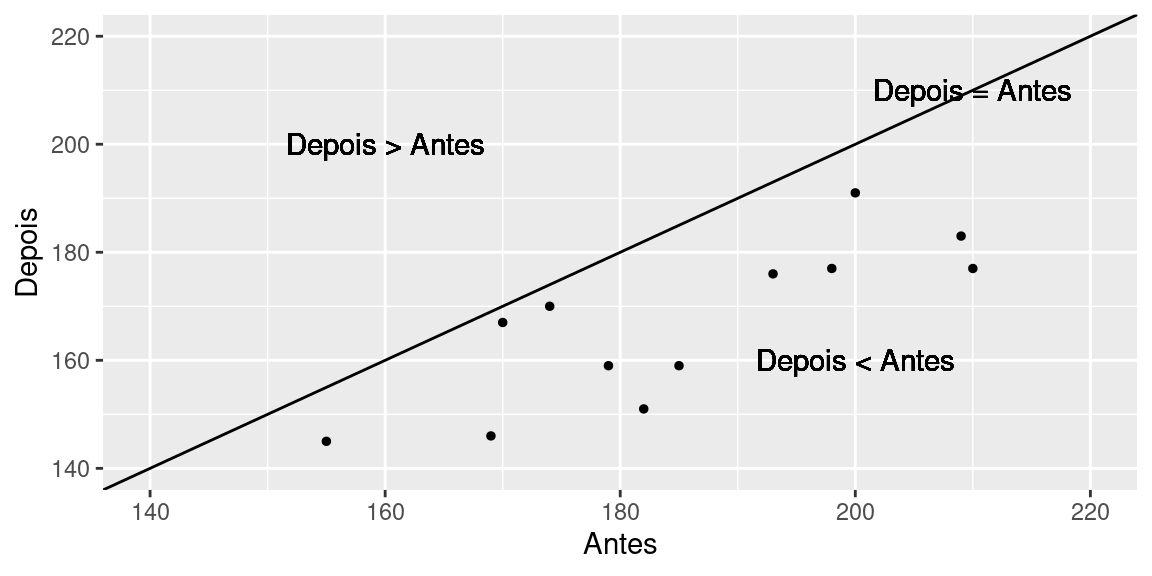
\includegraphics{inferencia_com_R_files/figure-latex/unnamed-chunk-43-1} \end{center}

De maneira geral, um gráfico de linhas deve ser construído de modo que:

\begin{itemize}
\tightlist
\item
  O início do eixo vertical seja o valor mínimo possível para a variável que está sendo representada, para evitar as distorções
\item
  O final do eixo vertical seja tal que a série fica centrada em relação ao eixo vertical
\item
  Os tamanhos dos eixos sejam o mais parecidos possível
\end{itemize}

\hypertarget{gruxe1fico-de-radar}{%
\section{Gráfico de Radar}\label{gruxe1fico-de-radar}}

O gráfico de radar é um diagrama e/ou gráfico que consiste de uma sequência de raios equi-angulares, com cada raio representando uma das variáveis. O comprimento de cada raio é proporcional à magnitude da variável para o ponto de dados em relação à máxima magnitude da variável em todos os pontos. Uma linha é desenhada ligando os valores de cada raio. Isso dá ao diagrama uma aparência de estrela, o que deu origem a um dos nomes mais populares para este gráfico. O gráfico de estrela pode ser usado para responder as seguintes questões:

\begin{itemize}
\tightlist
\item
  Que observações são mais semelhantes, por exemplo, existem clusters de observações?
\item
  Existem exceções?
\end{itemize}

Gráficos de radar oferecem uma maneira útil de exibir observações multivariáveis com um número arbitrário de variáveis. Cada estrela representa uma única observação. Normalmente, os gráficos de radar são gerados em um formato multi-diagrama com muitas estrelas em cada página, cada estrela representando uma observação. É um pouco mais fácil de ver padrões em dados se as observações forem organizadas em alguma ordem não-arbitrária (se as variáveis forem atribuídas aos raios da estrela em uma ordem significativa).

Uma aplicação de gráficos de radar é o controle de melhoria de qualidade para apresentar as métricas de desempenho de qualquer programa em curso. Eles também são usados em esportes para representar os pontos fortes e fracos de jogadores, onde eles são geralmente chamados de gráficos de aranha. No exemplo abaixo vemos a performance de três alunos (a,b,c) em relação as dimensões matemática, inglês, biologia, música e R.

\begin{Shaded}
\begin{Highlighting}[]
\FunctionTok{library}\NormalTok{(fmsb)}

\NormalTok{dados }\OtherTok{=} \FunctionTok{as.data.frame}\NormalTok{(}\FunctionTok{matrix}\NormalTok{(}\FunctionTok{sample}\NormalTok{(}\DecValTok{0}\SpecialCharTok{:}\DecValTok{20}\NormalTok{, }\DecValTok{15}\NormalTok{, }\AttributeTok{replace=}\NormalTok{F), }\AttributeTok{ncol=}\DecValTok{5}\NormalTok{))}
\FunctionTok{colnames}\NormalTok{(dados) }\OtherTok{=} \FunctionTok{c}\NormalTok{(}\StringTok{"matemática"}\NormalTok{, }\StringTok{"inglês"}\NormalTok{, }\StringTok{"biologia"}\NormalTok{, }\StringTok{"música"}\NormalTok{ ,}\StringTok{"R"}\NormalTok{)}
\FunctionTok{rownames}\NormalTok{(dados) }\OtherTok{=} \FunctionTok{paste}\NormalTok{(}\StringTok{"aluno"}\NormalTok{, letters[}\DecValTok{1}\SpecialCharTok{:}\DecValTok{3}\NormalTok{])}

\NormalTok{dados }\OtherTok{=} \FunctionTok{rbind}\NormalTok{(}\FunctionTok{rep}\NormalTok{(}\DecValTok{20}\NormalTok{,}\DecValTok{5}\NormalTok{), }\FunctionTok{rep}\NormalTok{(}\DecValTok{0}\NormalTok{,}\DecValTok{5}\NormalTok{), dados)}
 
\FunctionTok{radarchart}\NormalTok{(dados)}
\end{Highlighting}
\end{Shaded}

\begin{center}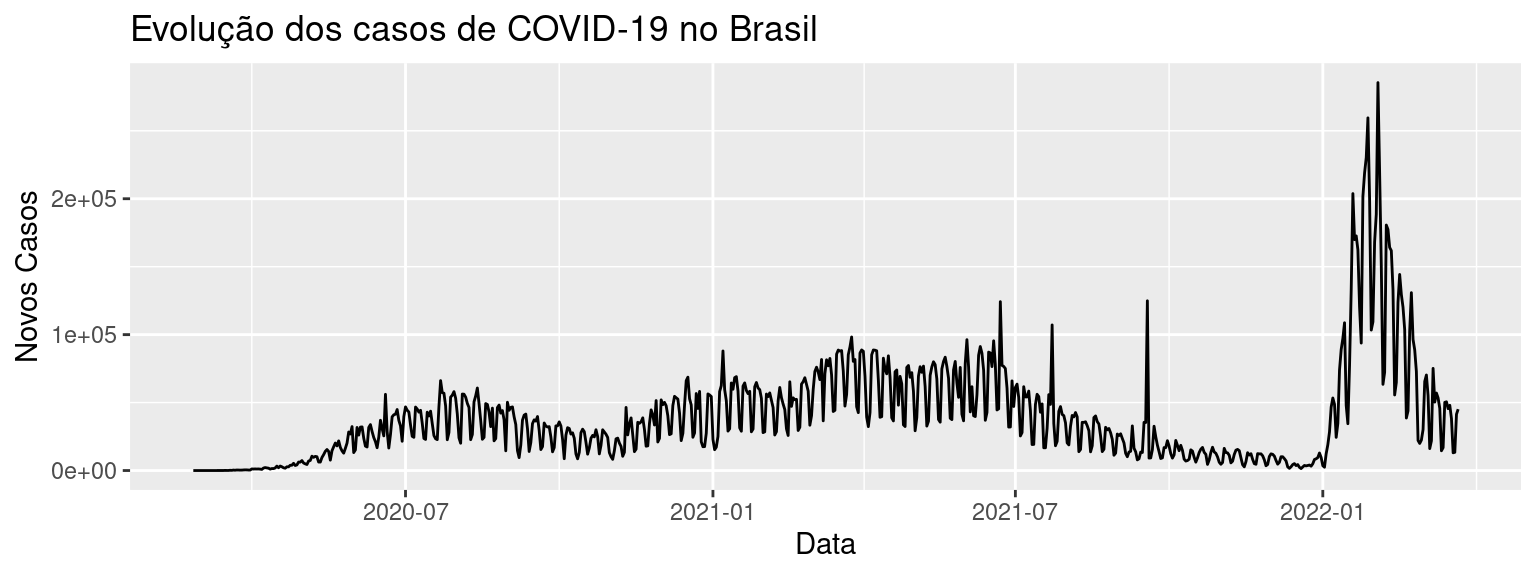
\includegraphics{inferencia_com_R_files/figure-latex/unnamed-chunk-44-1} \end{center}

\hypertarget{conceitos-buxe1sicos}{%
\chapter{Conceitos Básicos}\label{conceitos-buxe1sicos}}

\hypertarget{introduuxe7uxe3o-2}{%
\section{Introdução}\label{introduuxe7uxe3o-2}}

No estudo da inferência estatística, o objetivo principal é obter informações sobre uma população a partir das informações de uma amostra e aqui vamos precisar de definições mais formais de população e amostra. Para facilitar a compreensão destes conceitos, apresentamos o exemplo abaixo a título de ilustração

Em um estudo antropométrico em nível nacional, uma amostra de 5000 adultos é selecionada dentre os adultos brasileiros e uma das variáveis de estudo é a altura.

Neste exemplo, a população é o conjunto de todos os brasileiros adultos. No entanto, o interesse (um deles, pelo menos) está na altura dos brasileiros. Assim, nesse estudo, a cada sujeito da população associamos um número correspondente à sua altura. Se determinado sujeito é sorteado para entrar na amostra, o que nos interessa é esse número, ou seja, sua altura.

Como sabemos, essa é a definição de variável aleatória: uma função que associa a cada ponto do espaço amostral um número real. Dessa forma, a nossa população pode ser representada pela variável aleatória \(X\) = ``altura do adulto brasileiro''. Como essa é uma v.a. contínua, a ela está associada uma função de densidade de probabilidade \(f\) e da literatura, sabemos que é razoável supor que essa densidade seja a densidade normal. Assim, nossa população, nesse caso, é representada por uma v.a. \(X\sim N(\mu; \sigma^2)\). Conhecendo os valores de \(\mu\) e \(\sigma\) teremos informações completas sobre a nossa população.

Uma forma de obtermos os valores de \(\mu\) e \(\sigma\) é medindo as alturas de todos os brasileiros adultos. Mas esse seria um procedimento caro e demorado. Uma solução, então, é retirar uma amostra (subonjunto) da população e estudar essa amostra. Suponhamos que essa amostra seja retirada com reposição e que os sorteios sejam feitos de forma independente, isto é, o resultado de cada extração não altera o resultado das demais extrações. Ao sortearmos o primeiro elemento, estamos realizando um experimento que dá origem à v.a. \(X_1=\) altura do primeiro elemento; o segundo elemento dá origem à v.a. \(X_2=\) ``altura do segundo elemento'' e assim por diante. Como as extrações são feitas com reposição, todas as v.a. \(X_1, X_2, \ldots\) têm a mesma distribuição, que reflete a distribuição da altura de todos os brasileiros adultos. Para uma amostra específica, temos os valores observados \(x_1, x_2, \ldots\) dessas variáveis aleatórias.

\hypertarget{populauxe7uxe3o}{%
\section{População}\label{populauxe7uxe3o}}

A inferência estatística trata do problema de se obter informação sobre uma população a partir de uma amostra. Embora a população real possa ser constituída de pessoas, empresas, animais etc., as pesquisas estatísticas buscam informações sobre determinadas características dos sujeitos, características essas que podem ser representadas por números. Sendo assim, a cada sujeito da população está associado um número, o que nos permite apresentar a seguinte definição.

\textbf{População:} \emph{A população de uma pesquisa estatística pode ser representada por uma variável aleatória $X$ que descreve a característica de interesse.}

Os métodos de inferência nos permitirão obter estimativas dos parâmetros (característica de interesse) de tal variável aleatória, que pode ser contínua ou discreta.

\hypertarget{amostra}{%
\section{Amostra}\label{amostra}}

Embora existam vários métodos de seleção de amostras, nosso foco é a amostragem aleatória simples. Segundo tal método, toda amostra de mesmo tamanho \(n\) tem igual chance (probabilidade) de ser sorteada. É possível extrair amostras aleatórias simples com e sem reposição. No entanto, para populações grandes - ou infinitas - extrações com e sem reposição não levam a resultados muito diferentes. Assim, no estudo da Inferência Estatística, estaremos lidando sempre com amostragem aleatória simples com reposição. Este método de seleção atribui a cada elemento da população a mesma probabilidade de ser selecionado e esta probabilidade se mantém constante ao longo do processo de seleção da amostra (se as extrações fossem sem reposição isso não aconteceria). No restante desse curso omitiremos a expressão ``com reposição'', ou seja, o termo amostragem (ou amostra) aleatória simples sempre se referirá à amostragem com reposição. Por simplicidade, muitas vezes abreviaremos o termo amostra aleatória simples por aas.

Uma forma de se obter uma amostra aleatória simples é escrever os números ou nomes dos elementos da população em cartões iguais, colocar estes cartões em uma urna misturando-os bem e fazer os sorteios necessários, tendo o cuidado de colocar cada cartão sorteado na urna antes do próximo sorteio. Na prática, em geral são usados programas de computador, uma vez que as populações tendem a ser muito grandes.

Agora vamos formalizar o processo de seleção de uma amostra aleatória simples, de forma a relacioná-lo com os problemas de inferência estatística que iremos estudar. Seja uma população representada por uma variável aleatória \(X\). De tal população será sorteada uma amostra aleatória simples com reposição de tamanho \(n\). Como visto nos exemplos anteriores, cada sorteio dá origem a uma variável aleatória \(X_i\) e, como os sorteios são com reposição, todas essas variáveis têm a mesma distribuição de \(X\). Isso nos leva à seguinte definição.

\textbf{Amostra:} \emph{Uma amostra aleatória simples (aas) de tamanho $n$ de uma v.a. $X$ (população) é um conjunto de $n$ v.a. $X_1, X_2, \ldots, X_n$ independentes e identicamente
distribuídas (i.i.d.).}

É interessante notar a convenção usual: o valor observado de uma v.a. \(X\) é representado pela letra minúscula correspondente. Assim, depois do sorteio de uma aas de tamanho \(n\), temos valores observados \(x_1, x_2, \ldots, x_n\) das respectivas variáveis aleatórias.

\hypertarget{estatuxedsticas-e-paruxe2metros}{%
\section{Estatísticas e Parâmetros}\label{estatuxedsticas-e-paruxe2metros}}

Obtida uma aas, é possível calcular diversas características desta amostra, como, por exemplo, a média, a mediana, a variância, etc. Qualquer uma destas características é uma função de \(X_1, X_2, \ldots, X_n\) e, portanto, o seu valor depende da amostra sorteada. Sendo assim, cada uma dessas características ou funções é também uma v.a.. Por exemplo, a média amostral é a v.a. definida por \[\bar X = \frac{X_1+X_2+\ldots+X_n}{n}.\]

Temos, então, a seguinte definição:

\textbf{Estatística:} \emph{Uma estatística amostral ou estimador $T$ é qualquer função da
amostra $X_1, X_2, \ldots, X_n$, isto é, $T = g(X_1, X_2, \ldots, X_n)$ onde $g$ é uma função qualquer.}

As estatísticas amostrais que estaremos considerando neste curso são:

\begin{itemize}
\tightlist
\item
  média amostral: \(\bar X = \frac{1}{n}\sum_{i=1}^n X_i\)
\item
  variância amostral: \(S^2=\frac{1}{n-1}\sum_{i=1}^n (X_i-\bar X)^2\)
\end{itemize}

Para uma amostra específica, o valor obido para o estimador será denominado estimativa e, em geral, serão representadas por letras minúsculas. Por exemplo, temos as seguintes notações correspondentes à média amostral e à variância: \(\bar x\) e \(s^2\).

Outras estatísticas possíveis são o mínimo amostral, o máximo amostral, a amplitude amostral, etc.

De forma análoga, temos as características de interesse da população. No entanto, para diferenciar entre as duas situações (população e amostra), atribuimos nomes diferentes.

\textbf{Parâmetro:} \emph{Um parâmetro é uma característica da população.}

Assim, se a população é representada pela v.a. \(X\), alguns parâmetros são a esperança \(E(X)\) e a variância \(V(X)\). Com relação às características mais usuais, vamos usar a seguinte notação:

\begin{longtable}[]{@{}lll@{}}
\toprule
Característica & Parâmetro (população) & Estatística (amostra) \\
\midrule
\endhead
Média & \(\mu\) & \(\bar X\) \\
Variância & \(\sigma^2\) & \(S^2\) \\
Número de elementos & \(N\) & \(n\) \\
\bottomrule
\end{longtable}

\hypertarget{distribuiuxe7uxf5es-amostrais}{%
\section{Distribuições Amostrais}\label{distribuiuxe7uxf5es-amostrais}}

Nos problemas de inferência, estamos interessados em estimar um parâmetro \(\theta\) da população (por exemplo, a média populacional) através de uma aas \(X_1, X_2, \ldots, X_n\). Para isso, usamos uma estatística \(T\) (por exemplo, a média amostral) e, com base no valor obtido para \(T\) a partir de uma particular amostra, iremos tomar as decisões que o problema exige. Já foi dito que \(T\) é uma v.a., uma vez que depende da amostra sorteada; amostras diferentes fornecerão diferentes valores para \(T\).

Consideremos o seguinte exemplo, onde nossa população é o conjunto \(\{1,3,6,8\}\), isto é, este é o conjunto dos valores da característica de interesse da população em estudo. Assim, para esta população, ou seja, para essa v.a. \(X\) temos \(E(X)=\) 4.5 e \(V(X)=\) 7.25.

Suponha que dessa população iremos extrair uma aas de tamanho 2 e a estatística que iremos calcular é a média amostral. Algumas possibilidades de amostra são \(\{1,1\}\), \(\{1,3\}\), \(\{6,8\}\), para as quais os valores da média amostral são \(1\), \(2\) e \(7\), respectivamente. Podemos ver, então, que há uma variabilidade nos valores da estatística e, assim, seria interessante que conhecêssemos tal variabilidade. Conhecendo tal variabilidade, temos condições de saber ``quão infelizes'' podemos ser no sorteio da amostra. No exemplo acima, as amostras \(\{1,1\}\) e \(\{8,8\}\) são as que têm média amostral mais afastada da verdadeira média populacional. Se esses valores tiverem chance muito mais alta do que os valores mais próximos de \(E(X)\), podemos ter sérios problemas.

Para conhecer o comportamento (distribuição) da média amostral, teríamos que conhecer todos os possíveis valores de \(X\), o que equivaleria a conhecer todas as possíveis amostras de tamanho 2 de tal população. Nesse exemplo, como só temos 4 elementos na população, a obtenção de todas as aas de tamanho 2 não é difícil. No entanto, para um número um pouco maior dele elementos, ou quando não conhecemos todo o espaço amostral, essa tarefa se torna complexa.

\textbf{Distribuição de Probabilidade:}\emph{A função de distribuição amostral de uma estatística $T$ é a função de distribuição de probabilidades de $T$ ao longo de todas as possíveis amostras de tamanho $n$.}

Em outras palavras, uma distribuição amostral é a distribuição de probabilidades de uma medida estatística baseada em uma amostra aleatória. Ao retirar uma amostra aleatória de uma população estaremos considerando cada valor da amostra como um valor de uma variável aleatória cuja distribuição de probabilidade é a mesma da população no instante da retirada desse elemento para a amostra. Em consequência do fato de os valores de amostra serem aleatórios, decorre que qualquer quantidade calculada em função dos elementos da amostra também será uma variável aleatória.

Podemos ver que a obtenção da distribuição amostral de qualquer estatística \(T\) é um processo tão ou mais complicado do que trabalhar com a população inteira. Na prática, o que temos é uma única amostra e com esse resultado é que temos que tomar as decisões pertinentes ao problema em estudo. Esta tomada de decisão, no entanto, será facilitada se conhecermos resultados teóricos sobre o comportamento da distribuição amostral.

\hypertarget{propriedades-dos-estimadores}{%
\section{Propriedades dos Estimadores}\label{propriedades-dos-estimadores}}

Vimos anteriormente que, dada uma população, existem muitas e muitas aas de tamanho \(n\) que podem ser sorteadas. Cada uma dessas amostras resulta em um valor diferente da estatística de interesse (\(\bar X\) e \(S^2\), por exemplo). O que esses resultados estão mostrando é como esses diferentes valores se comportam em relação ao verdadeiro (mas desconhecido) valor do parâmetro.

Considere a Figura abaixo, onde o alvo representa o valor do parâmetro e os ``tiros'', indicados pelos símbolo x, representam os diferentes valores amostrais da estatística de interesse.

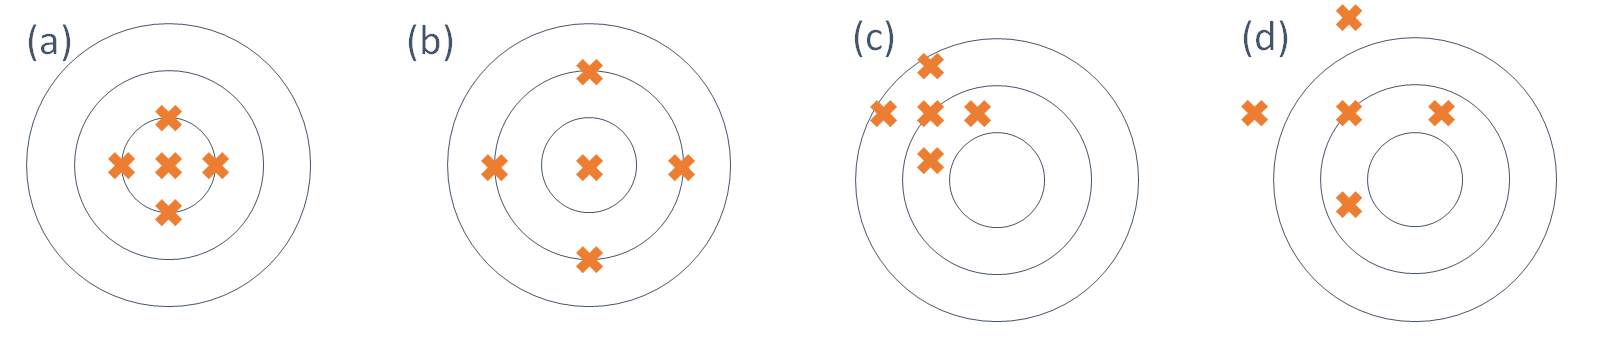
\includegraphics{Estimadores_exemplo.png}

Nas partes (a) e (b) da figura, os tiros estão em torno do alvo, enquanto nas partes (c) e (d) isso não acontece. Comparando as partes (a) e (b), podemos ver que na parte (a) os tiros estão mais concentrados em torno do alvo, isto é, têm menor dispersão. Isso reflete uma pontaria mais certeira do atirador em (a). Analogamente, nas partes (c) e (d), embora ambos os atiradores estejam com a mira deslocada, os tiros do atirador (c) estão mais concentrados em torno de um alvo; o deslocamento poderia até ser resultado de um desalinhamento da arma. Já o atirador (d), além de estar com o alvo deslocado, ele tem os tiros mais espalhados, o que reflete menor precisão.

Traduzindo esta situação para o contexto de estimadores e suas propriedades, temos o seguinte: nas partes (a) e (b), temos dois estimadores que fornecem estimativas centradas em torno do verdadeiro valor do parâmetro, ou seja, as diferentes amostras fornecem valores distribuídos em torno do verdadeiro valor do parâmetro. A diferença é que em (b) esses valores estão mais dispersos e, assim, temos mais chance de obter uma amostra ``infeliz'', ou seja, uma amostra que forneça um resultado muito afastado do valor do parâmetro. Essas duas propriedades estão associadas à esperança e à variância do estimador, que são medidas de centro e dispersão, respectivamente. Nas partes (c) e (d), as estimativas estão centradas em torno de um valor diferente do parâmetro de interesse e na parte (d), a dispersão é maior.

Temos, assim, ilustrados os seguintes conceitos:

\textbf{Viés:}\emph{Um estimador $T$ é dito um estimador não-viesado do parâmetro $\theta$ se $E(T)=\theta$.}

Essa esperança é calculada ao longo de todas as possíveis amostras, ou seja, é a esperança da distribuição amostral de \(T\). Nas partes (a) e (b) da Figura os estimadores são não-viesados e nas partes (c) e (d), os estimadores são viesados.

Com relação aos estimadores \(bar X\), \(S^2\) e \(\hat \sigma^2\), veremos formalmente que os dois primeiros são não-viesados para estimar a média e a variância populacionais, respectivamente, enquanto \(\hat \sigma^2\) é viesado para estimar a variância populacional. Essa é a razão para se usar \(S^2\), e não \(\hat \sigma^2\).

\textbf{Eficiência:}\emph{Se $T_1$ e $T_2$ são dois estimadores não-viesados do parâmetro $\theta$, diz-se que $T_1$ é mais eficiente que $T_2$ se $V(T_1)<V(T_2)$.}

Na Figura, o estimador da parte (a) é mais eficiente que o estimador da parte (b). Uma outra propriedade dos estimadores está relacionada à idéia bastante intuitiva de que à medida que se aumenta o tamanho da amostra, mais perto devemos ficar do verdadeiro valor do parâmetro.

\textbf{Consistência:}\emph{Um estimador $T$ de um parâmetro $\theta$ é consistente se:}

\begin{itemize}
\tightlist
\item
  \(\lim_{n\to\infty} E(\hat\theta)=\theta\)
\item
  \(\lim_{n\to\infty} V(\hat\theta)=0\)
\end{itemize}

\hypertarget{distribuiuxe7uxf5es-amostrais-1}{%
\chapter{Distribuições Amostrais}\label{distribuiuxe7uxf5es-amostrais-1}}

\hypertarget{introduuxe7uxe3o-3}{%
\section{Introdução}\label{introduuxe7uxe3o-3}}

Uma distribuição amostral é a distribuição de probabilidades de uma medida estatística baseada em uma amostra aleatória. Ao retirar uma amostra aleatória de uma população estaremos considerando cada valor da amostra como um valor de uma variável aleatória cuja distribuição de probabilidade é a mesma da população no instante da retirada desse elemento para a amostra. Em consequência do fato de os valores de amostra serem aleatórios, decorre que qualquer quantidade calculada em função dos elementos da amostra também será uma variável aleatória

\hypertarget{distribuiuxe7uxe3o-amostral-da-muxe9dia-amostral}{%
\section{Distribuição Amostral da Média Amostral}\label{distribuiuxe7uxe3o-amostral-da-muxe9dia-amostral}}

Considere \(X_1,\ldots,X_n\) uma amostra aleatória de uma distribuição normal com média \(\mu\) e variância \(\sigma^2\).

Tomamos, por exemplo, o problema de estimar quantas horas adicionais de sono são garantidas a um indivíduo após ingerir uma determinada droga. Além disso, suponha que a droga é testada em 20 indivíduos de modo que a média amostral seja \(\bar X=0,8\) horas. Porém, se o estudo for repetido com outros 20 participantes podemos ter outros resultados para a média amostral. Por exemplo, podemos ter \(\bar X=1,3\). E, repetindo o estudo novamente, poderíamos ter \(\bar X=-0,2\). Em termos estatísticos, haverá variação entre as médias amostrais.

Este problema poderia ser resolvido se repetíssemos o estudo infinitas vezes, porém isto é inviável.

Quando as observações são amostradas aleatoriamente de uma distribuição normal, a média amostral também tem uma distribuição normal. Isto é, quando \(n\) observações são amostradas aleatoriamente de uma distribuição normal com média \(\mu\) e variância \(\sigma^2\), a média amostral tem distribuição normal com média \(\mu\) e variância \(\frac{\sigma^2}{n}\). Ou seja, se

\[X\sim N(\mu,\sigma^2)\text{, então} \bar X \sim N\left(\mu,\frac{\sigma^2}{n}\right).\]

\hypertarget{visualizando}{%
\subsection{Visualizando}\label{visualizando}}

Considere uma população normal com média \(\mu=10\) e variância \(\sigma^2=4\). Vamos realizar um estudo de simulação para a distribuição da média amostral considerando amostras de tamanho 20 dessa população.

Primeiramente, considere que são retiradas 15 amostras de tamanho 20 dessa população.

\begin{Shaded}
\begin{Highlighting}[]
\FunctionTok{library}\NormalTok{(ggplot2)}
\NormalTok{n }\OtherTok{=} \DecValTok{15}
\NormalTok{matriz\_aux }\OtherTok{=} \FunctionTok{matrix}\NormalTok{(}\ConstantTok{NA}\NormalTok{,}\AttributeTok{nrow=}\DecValTok{20}\NormalTok{,}\AttributeTok{ncol=}\NormalTok{n)}
\ControlFlowTok{for}\NormalTok{(j }\ControlFlowTok{in} \DecValTok{1}\SpecialCharTok{:}\FunctionTok{ncol}\NormalTok{(matriz\_aux))\{matriz\_aux[,j]}\OtherTok{=}\FunctionTok{rnorm}\NormalTok{(}\DecValTok{20}\NormalTok{,}\AttributeTok{mean=}\DecValTok{10}\NormalTok{,}\AttributeTok{sd=}\DecValTok{2}\NormalTok{)\}}
\NormalTok{medias }\OtherTok{=} \FunctionTok{data.frame}\NormalTok{(}\AttributeTok{x=}\DecValTok{1}\SpecialCharTok{:}\FunctionTok{ncol}\NormalTok{(matriz\_aux),}\AttributeTok{y=}\FunctionTok{colMeans}\NormalTok{(matriz\_aux))}
\FunctionTok{ggplot}\NormalTok{(medias,}\FunctionTok{aes}\NormalTok{(y)) }\SpecialCharTok{+}
  \FunctionTok{geom\_histogram}\NormalTok{(}\AttributeTok{color =} \StringTok{"white"}\NormalTok{) }\SpecialCharTok{+}
  \FunctionTok{theme}\NormalTok{(}\AttributeTok{axis.title =} \FunctionTok{element\_blank}\NormalTok{())}
\end{Highlighting}
\end{Shaded}

\begin{center}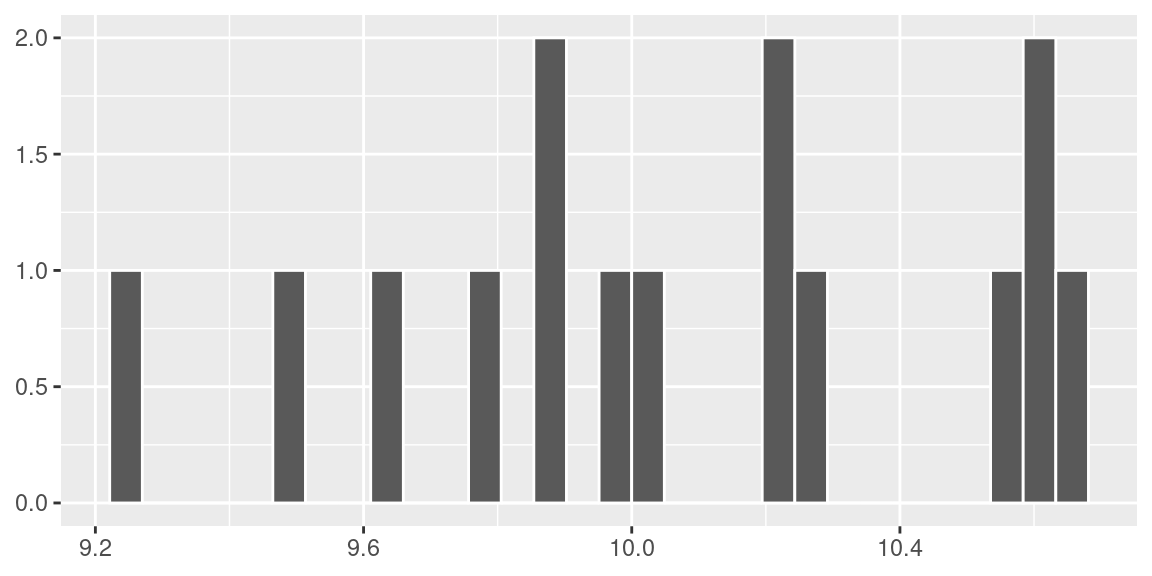
\includegraphics{inferencia_com_R_files/figure-latex/unnamed-chunk-47-1} \end{center}

Nessa simulação obtivemos \(\bar x =\) 9.99 e \(s =\) 0.3.

Suponha agora que façamos o mesmo processo, porém ao invés de considerarmos 15 amostras de tamanho 20, consideramos 200 amostras.

\begin{Shaded}
\begin{Highlighting}[]
\NormalTok{n }\OtherTok{=} \DecValTok{200}
\NormalTok{matriz\_aux }\OtherTok{=} \FunctionTok{matrix}\NormalTok{(}\ConstantTok{NA}\NormalTok{,}\AttributeTok{nrow=}\DecValTok{20}\NormalTok{,}\AttributeTok{ncol=}\NormalTok{n)}
\ControlFlowTok{for}\NormalTok{(j }\ControlFlowTok{in} \DecValTok{1}\SpecialCharTok{:}\FunctionTok{ncol}\NormalTok{(matriz\_aux))\{matriz\_aux[,j]}\OtherTok{=}\FunctionTok{rnorm}\NormalTok{(}\DecValTok{20}\NormalTok{,}\AttributeTok{mean=}\DecValTok{10}\NormalTok{,}\AttributeTok{sd=}\DecValTok{2}\NormalTok{)\}}
\NormalTok{medias }\OtherTok{=} \FunctionTok{data.frame}\NormalTok{(}\AttributeTok{x=}\DecValTok{1}\SpecialCharTok{:}\FunctionTok{ncol}\NormalTok{(matriz\_aux),}\AttributeTok{y=}\FunctionTok{colMeans}\NormalTok{(matriz\_aux))}
\FunctionTok{ggplot}\NormalTok{(medias,}\FunctionTok{aes}\NormalTok{(y)) }\SpecialCharTok{+}
  \FunctionTok{geom\_histogram}\NormalTok{(}\AttributeTok{color =} \StringTok{"white"}\NormalTok{) }\SpecialCharTok{+}
  \FunctionTok{theme}\NormalTok{(}\AttributeTok{axis.title =} \FunctionTok{element\_blank}\NormalTok{())}
\end{Highlighting}
\end{Shaded}

\begin{center}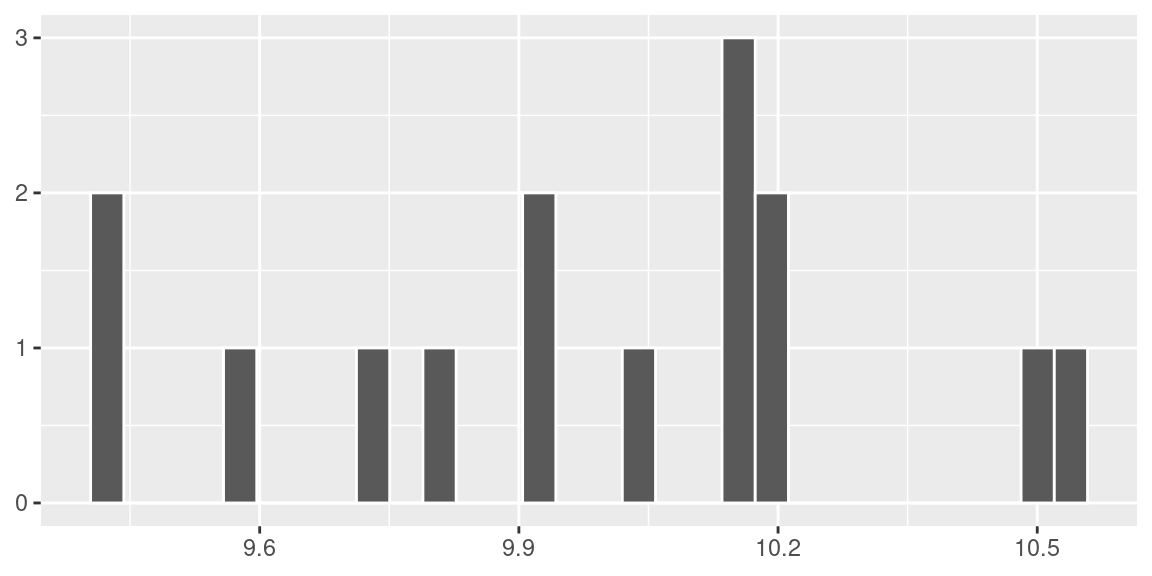
\includegraphics{inferencia_com_R_files/figure-latex/unnamed-chunk-48-1} \end{center}

Agora, obtivemos \(\bar x =\) 10.05 e \(s =\) 0.46.

Realizando o mesmo experimento, porém agora considerando 10000 amostras de tamanho 20, a distribuição da média amostral pode ser vista segundo o histograma abaixo.

\begin{Shaded}
\begin{Highlighting}[]
\NormalTok{n }\OtherTok{=} \DecValTok{10000}
\NormalTok{matriz\_aux }\OtherTok{=} \FunctionTok{matrix}\NormalTok{(}\ConstantTok{NA}\NormalTok{,}\AttributeTok{nrow=}\DecValTok{20}\NormalTok{,}\AttributeTok{ncol=}\NormalTok{n)}
\ControlFlowTok{for}\NormalTok{(j }\ControlFlowTok{in} \DecValTok{1}\SpecialCharTok{:}\FunctionTok{ncol}\NormalTok{(matriz\_aux))\{matriz\_aux[,j]}\OtherTok{=}\FunctionTok{rnorm}\NormalTok{(}\DecValTok{20}\NormalTok{,}\AttributeTok{mean=}\DecValTok{10}\NormalTok{,}\AttributeTok{sd=}\DecValTok{2}\NormalTok{)\}}
\NormalTok{medias }\OtherTok{=} \FunctionTok{data.frame}\NormalTok{(}\AttributeTok{x=}\DecValTok{1}\SpecialCharTok{:}\FunctionTok{ncol}\NormalTok{(matriz\_aux),}\AttributeTok{y=}\FunctionTok{colMeans}\NormalTok{(matriz\_aux))}
\FunctionTok{ggplot}\NormalTok{(medias,}\FunctionTok{aes}\NormalTok{(y)) }\SpecialCharTok{+}
  \FunctionTok{geom\_histogram}\NormalTok{(}\AttributeTok{color =} \StringTok{"white"}\NormalTok{) }\SpecialCharTok{+}
  \FunctionTok{theme}\NormalTok{(}\AttributeTok{axis.title =} \FunctionTok{element\_blank}\NormalTok{())}
\end{Highlighting}
\end{Shaded}

\begin{center}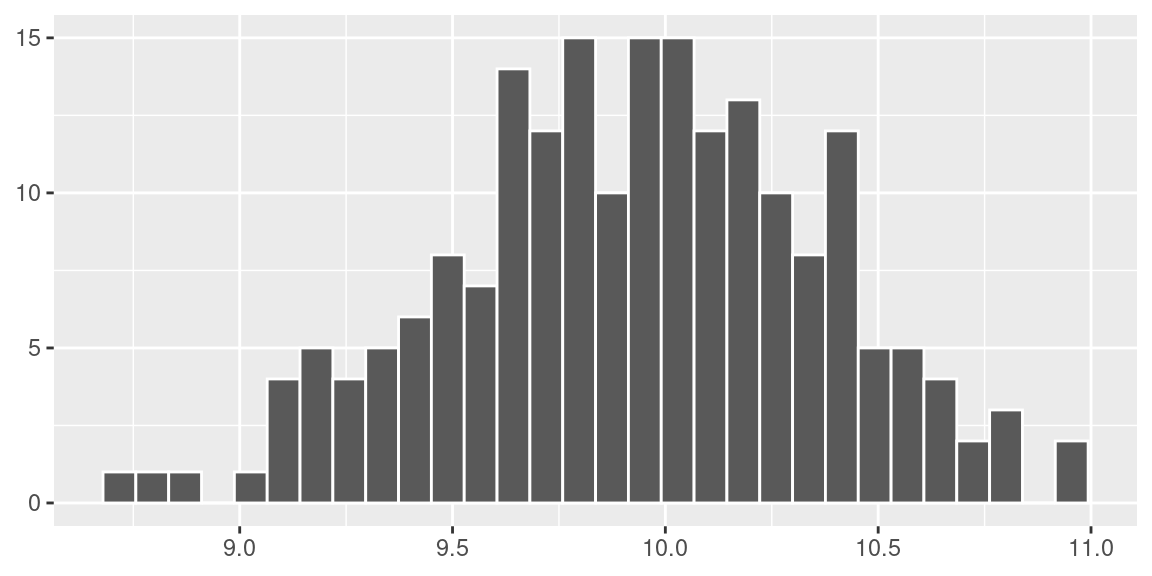
\includegraphics{inferencia_com_R_files/figure-latex/unnamed-chunk-49-1} \end{center}

Para este caso, a média das médias amostrais foi \(\bar x=\) 10 e o desvio padrão foi \(s =\) 0.44. Então, empiricamente, podemos perceber que a distribuição da média amostral se aproxima de uma distribuição normal com média \(\mu=10\) e desvio padrão \(\frac{\sigma}{\sqrt{n}}=\frac{2}{\sqrt{20}}=0,4472\).

\hypertarget{prova}{%
\subsection{Prova}\label{prova}}

Para provar que se \(X\sim N(\mu,\sigma^2)\), então \(\bar X \sim N(\mu,\frac{\sigma^2}{n})\), vamos precisar de somente três passos.

\begin{enumerate}
\def\labelenumi{\arabic{enumi}.}
\tightlist
\item
  Dado que \(\bar X = \frac{1}{n}\sum_{i=1}^{n}X_i\), onde \(X_1,\ldots,X_n\) é uma amostra aleatória de tamanho \(n\) de uma população Normal sabemos que combinação linear de Normais resulta em também uma distribuição Normal, portanto daqui temos que \(\bar X \sim Normal\);
\item
  Se \(\bar X = \frac{1}{n}\sum_{i=1}^{n}X_i\), então \[E\left[\bar X\right] = E\left[\frac{1}{n}\sum_{i=1}^{n}X_i\right]=\frac{1}{n}\sum_{i=1}^{n}E\left[X_i\right]=\frac{n\mu}{n}=\mu\]
\item
  Por fim, se \(\bar X = \frac{1}{n}\sum_{i=1}^{n}X_i\), então como os \(X_i\)'s são independentes \[V \left[\bar X\right] = V\left[\frac{1}{n}\sum_{i=1}^{n}X_i\right]=\frac{1}{n^2}\sum_{i=1}^{n}V\left[X_i\right]=\frac{n\sigma^2}{n^2}=\frac{\sigma^2}{n}\]
\end{enumerate}

\hypertarget{teorema-central-do-limite}{%
\section{Teorema Central do Limite}\label{teorema-central-do-limite}}

Os resultados vistos anteriormente são válidos para populações normais, isto é, se uma população é normal com média \(\mu\) e variância \(\sigma^2\), então a distribuição amostral de \(\bar X\) é também normal com média \(\mu\) e variância \(\frac{\sigma^2}{n}\), onde \(n\) é o tamanho da amostra. O Teorema Central do Limite (TCL) nos fornece um resultado análogo para qualquer distribuição populacional, desde que o tamanho da amostra seja suficientemente grande.

Seja \(X_1,\ldots,X_n\) uma amostra aleatória simples de uma população \(X\) tal que \(E(X)=\mu\) e \(V(X)=\sigma^2\). Então, a distribuição de \(\bar X\) converge para a distribuição Normal com média \(\mu\) e variância \(\frac{\sigma^2}{n}\) quando \(n\rightarrow \infty\). Equivalentemente, \[\frac{\bar X-\mu}{\frac{\sigma}{\sqrt{n}}}\rightarrow N(0,1)\]

A interpretação prática do TCL é a seguinte: para amostras ``grandes'' de qualquer população, podemos aproximar a distribuição amostral de \(\bar X\) por uma distribuição normal com a mesma média populacional e variância igual à variância populacional dividida pelo tamanho da amostra.

Quão grande deve ser a amostra para se obter uma boa aproximação depende das características da distribuição populacional. Se a distribuição populacional não se afastar muito de uma distribuição normal, a aproximação será boa, mesmo para tamanhos pequenos de amostra. Em termos práticos, esse teorema é de extrema importância, daí ser chamado de Teorema Central e, em geral, amostras de tamanho \(n>30\) já fornecem uma aproximação razoável.

\hypertarget{visualizando-1}{%
\subsection{Visualizando}\label{visualizando-1}}

Considere uma população exponencial com média \(\mu=1\), ou seja, uma população distribuída segundo uma exponencial com parâmetro \(\lambda=1\).

O gráfico superior representa a distribuição populacional e os histogramas representam a distribuição amostral de \(\bar X\) ao longo de 5000 amostras de tamanhos 10, 50, 100 e 250. Assim, podemos ver que, embora a população seja completamente diferente da normal, a distribuição amostral de \(\bar X\) vai se tornando cada vez mais próxima da normal à medida que \(n\) aumenta.

\begin{Shaded}
\begin{Highlighting}[]
\NormalTok{matriz\_aux\_10 }\OtherTok{=} \FunctionTok{matrix}\NormalTok{(}\ConstantTok{NA}\NormalTok{,}\AttributeTok{nrow=}\DecValTok{5000}\NormalTok{,}\AttributeTok{ncol=}\DecValTok{10}\NormalTok{)}
\NormalTok{matriz\_aux\_50 }\OtherTok{=} \FunctionTok{matrix}\NormalTok{(}\ConstantTok{NA}\NormalTok{,}\AttributeTok{nrow=}\DecValTok{5000}\NormalTok{,}\AttributeTok{ncol=}\DecValTok{50}\NormalTok{)}
\NormalTok{matriz\_aux\_100 }\OtherTok{=} \FunctionTok{matrix}\NormalTok{(}\ConstantTok{NA}\NormalTok{,}\AttributeTok{nrow=}\DecValTok{5000}\NormalTok{,}\AttributeTok{ncol=}\DecValTok{100}\NormalTok{)}
\NormalTok{matriz\_aux\_250 }\OtherTok{=} \FunctionTok{matrix}\NormalTok{(}\ConstantTok{NA}\NormalTok{,}\AttributeTok{nrow=}\DecValTok{5000}\NormalTok{,}\AttributeTok{ncol=}\DecValTok{250}\NormalTok{)}
\ControlFlowTok{for}\NormalTok{(j }\ControlFlowTok{in} \DecValTok{1}\SpecialCharTok{:}\FunctionTok{ncol}\NormalTok{(matriz\_aux\_10))\{matriz\_aux\_10[,j]}\OtherTok{=}\FunctionTok{rexp}\NormalTok{(}\DecValTok{5000}\NormalTok{,}\AttributeTok{rate=}\DecValTok{1}\NormalTok{)\}}
\ControlFlowTok{for}\NormalTok{(j }\ControlFlowTok{in} \DecValTok{1}\SpecialCharTok{:}\FunctionTok{ncol}\NormalTok{(matriz\_aux\_50))\{matriz\_aux\_50[,j]}\OtherTok{=}\FunctionTok{rexp}\NormalTok{(}\DecValTok{5000}\NormalTok{,}\AttributeTok{rate=}\DecValTok{1}\NormalTok{)\}}
\ControlFlowTok{for}\NormalTok{(j }\ControlFlowTok{in} \DecValTok{1}\SpecialCharTok{:}\FunctionTok{ncol}\NormalTok{(matriz\_aux\_100))\{matriz\_aux\_100[,j]}\OtherTok{=}\FunctionTok{rexp}\NormalTok{(}\DecValTok{5000}\NormalTok{,}\AttributeTok{rate=}\DecValTok{1}\NormalTok{)\}}
\ControlFlowTok{for}\NormalTok{(j }\ControlFlowTok{in} \DecValTok{1}\SpecialCharTok{:}\FunctionTok{ncol}\NormalTok{(matriz\_aux\_250))\{matriz\_aux\_250[,j]}\OtherTok{=}\FunctionTok{rexp}\NormalTok{(}\DecValTok{5000}\NormalTok{,}\AttributeTok{rate=}\DecValTok{1}\NormalTok{)\}}
\NormalTok{medias\_10 }\OtherTok{=} \FunctionTok{data.frame}\NormalTok{(}\AttributeTok{x=}\DecValTok{1}\SpecialCharTok{:}\FunctionTok{ncol}\NormalTok{(matriz\_aux\_10),}\AttributeTok{y=}\FunctionTok{colMeans}\NormalTok{(matriz\_aux\_10),}\AttributeTok{label=}\StringTok{"id\_10"}\NormalTok{)}
\NormalTok{medias\_50 }\OtherTok{=} \FunctionTok{data.frame}\NormalTok{(}\AttributeTok{x=}\DecValTok{1}\SpecialCharTok{:}\FunctionTok{ncol}\NormalTok{(matriz\_aux\_50),}\AttributeTok{y=}\FunctionTok{colMeans}\NormalTok{(matriz\_aux\_50),}\AttributeTok{label=}\StringTok{"id\_50"}\NormalTok{)}
\NormalTok{medias\_100 }\OtherTok{=} \FunctionTok{data.frame}\NormalTok{(}\AttributeTok{x=}\DecValTok{1}\SpecialCharTok{:}\FunctionTok{ncol}\NormalTok{(matriz\_aux\_100),}\AttributeTok{y=}\FunctionTok{colMeans}\NormalTok{(matriz\_aux\_100),}\AttributeTok{label=}\StringTok{"id\_100"}\NormalTok{)}
\NormalTok{medias\_250 }\OtherTok{=} \FunctionTok{data.frame}\NormalTok{(}\AttributeTok{x=}\DecValTok{1}\SpecialCharTok{:}\FunctionTok{ncol}\NormalTok{(matriz\_aux\_250),}\AttributeTok{y=}\FunctionTok{colMeans}\NormalTok{(matriz\_aux\_250),}\AttributeTok{label=}\StringTok{"id\_250"}\NormalTok{)}
\NormalTok{tudo }\OtherTok{=} \FunctionTok{rbind}\NormalTok{(medias\_10,medias\_50,medias\_100,medias\_250)}
\NormalTok{tudo}\SpecialCharTok{$}\NormalTok{label }\OtherTok{=} \FunctionTok{factor}\NormalTok{(tudo}\SpecialCharTok{$}\NormalTok{label, }\AttributeTok{levels =} \FunctionTok{c}\NormalTok{(}\StringTok{"id\_10"}\NormalTok{, }\StringTok{"id\_50"}\NormalTok{, }\StringTok{"id\_100"}\NormalTok{, }\StringTok{"id\_250"}\NormalTok{))}
\FunctionTok{ggplot}\NormalTok{(tudo,}\FunctionTok{aes}\NormalTok{(y)) }\SpecialCharTok{+}
  \FunctionTok{geom\_histogram}\NormalTok{(}\FunctionTok{aes}\NormalTok{(}\AttributeTok{y=}\NormalTok{..density..),}\AttributeTok{color =} \StringTok{"white"}\NormalTok{) }\SpecialCharTok{+}
  \FunctionTok{facet\_wrap}\NormalTok{(}\SpecialCharTok{\textasciitilde{}}\NormalTok{label, }\AttributeTok{scales =} \StringTok{"free"}\NormalTok{) }\SpecialCharTok{+}
  \FunctionTok{theme}\NormalTok{(}\AttributeTok{axis.title =} \FunctionTok{element\_blank}\NormalTok{())}
\end{Highlighting}
\end{Shaded}

\begin{center}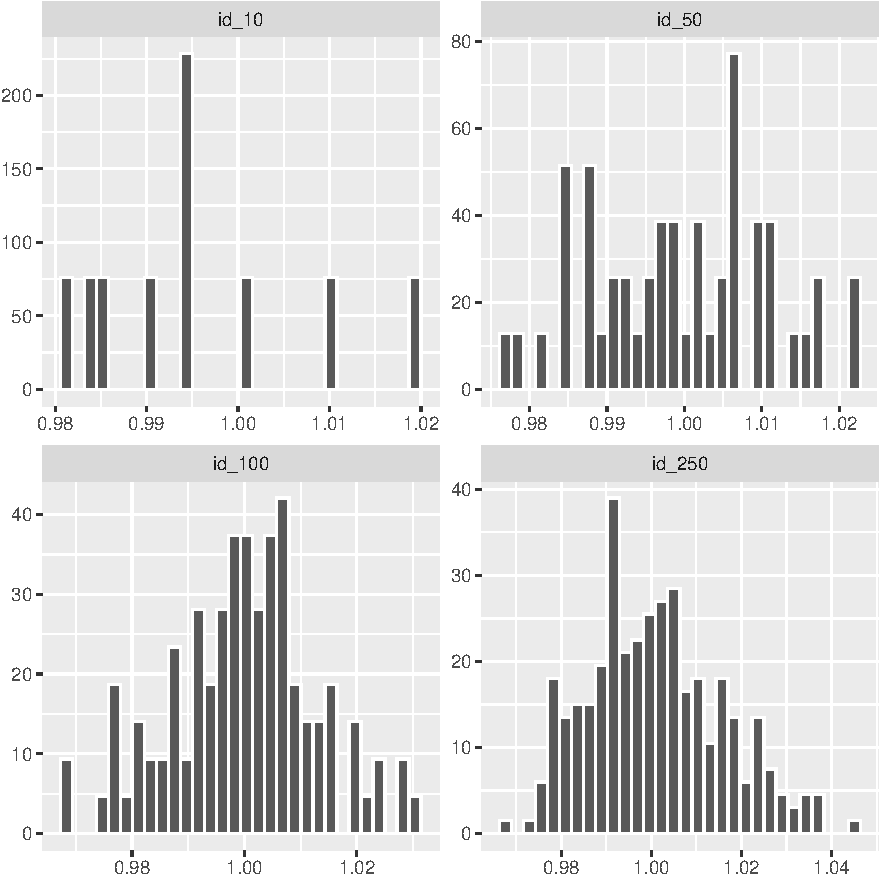
\includegraphics{inferencia_com_R_files/figure-latex/unnamed-chunk-50-1} \end{center}

\hypertarget{distribuiuxe7uxe3o-amostral-da-variuxe2ncia-amostral}{%
\section{Distribuição Amostral da Variância Amostral}\label{distribuiuxe7uxe3o-amostral-da-variuxe2ncia-amostral}}

Já vimos que a estatística \[S^2=\frac{1}{n-1}\sum_{i=1}^{n}\left(X_i-\bar X\right)^2\] é um estimador não viciado da variância \(\sigma^2\), portanto \[E(S^2)=\sigma^2\]. Vamos estudar agora a distribuição amostral de \(S^2\) e para isso precisamos estudar a distribuição qui-quadrado.

\hypertarget{distribuiuxe7uxe3o-qui-quadrado}{%
\subsection{Distribuição Qui-quadrado}\label{distribuiuxe7uxe3o-qui-quadrado}}

Se \(X\) é uma variável aleatória com densidade

\[f_X(x)=\frac{1}{\Gamma\big({\frac{k}{2}}\big)}\big(\frac{1}{2}\big)^{\frac{k}{2}}x^{\frac{k}{2}-1}e^{-\frac{x}{2}},k>0,x>0,\]

onde \(\Gamma(w)=\int_0^\infty x^{w-1}e^{-x}dx, w>0\). Então, \(X\) tem uma distribuição qui-quadrado com \(k\) graus de liberdade, onde o parâmetro \(k\) é um número inteiro.

Para entender a ideia de graus de liberdade, consideremos um conjunto de dados qualquer. Graus de liberdade é o número de valores deste conjunto de dados que podem variar após terem sido impostas certas restrições a todos os valores. Por exemplo, consideremos que 10 estudantes obtiveram em um teste média 8. Assim, a soma das 10 notas deve ser 80 (restrição). Portanto, neste caso, temos um grau de liberdade de \(10-1=9\), pois 9 notas podem variar livremente desde que a soma seja 80, no entanto 1 nota sempre será {[}80-(soma das 9 outras notas){]}.

Temos também que se as variáveis aleatórias \(X_i\), \(i=1,2,\ldots,n\) são independentes e normalmente distribuídas com médias \(\mu_i\) e variâncias \(\sigma^2_i\), isto é \(X_i\sim N(\mu_i,\sigma^2_i)\), então

\[U=\sum_{i=1}^{n}\left(\frac{X_i-\mu}{\sigma^2}\right)^2\]

tem uma distribuição qui-quadrado com \(n\) graus de liberdade.

Além disso, se \(X_1,\ldots,X_n\) é uma a.a. de uma distribuição normal padrão, então, valem as seguintes propriedades:

\begin{enumerate}
\def\labelenumi{(\roman{enumi})}
\item
  \(\bar X\) e \(\sum_{i=1}^{n}(X_i-\bar X)^2\) são independentes;
\item
  \(\sum_{i=1}^{n}(X_i-\bar X)^2\) tem uma distribuição qui-quadrado com \(n-1\) graus de liberdade.
\end{enumerate}

Assim, chegamos que se \(S^2\) é a variância amostral de uma amostra aleatória \(X_1,\ldots,X_n\) de uma distribuição normal com média \(\mu\) e variância \(\sigma^2\), então

\[U=\frac{(n-1)S^2}{\sigma^2}\sim \chi^2_{n-1},\]

ou seja, \(U\) tem uma distribuição qui-quadrado com \(n-1\) graus de liberdade.

\hypertarget{visualizando-2}{%
\subsection{Visualizando}\label{visualizando-2}}

Analogamente ao estudo de simulação realizado no caso da média amostral, considere uma população normal com média \(\mu=10\) e variância \(\sigma^2=4\).

Primeiramente, considere que são retiradas 15 amostras de tamanho 20 dessa população.

\begin{Shaded}
\begin{Highlighting}[]
\NormalTok{n }\OtherTok{=} \DecValTok{15}
\NormalTok{matriz\_aux }\OtherTok{=} \FunctionTok{matrix}\NormalTok{(}\ConstantTok{NA}\NormalTok{,}\AttributeTok{nrow=}\DecValTok{20}\NormalTok{,}\AttributeTok{ncol=}\NormalTok{n)}
\ControlFlowTok{for}\NormalTok{(j }\ControlFlowTok{in} \DecValTok{1}\SpecialCharTok{:}\FunctionTok{ncol}\NormalTok{(matriz\_aux))\{matriz\_aux[,j]}\OtherTok{=}\FunctionTok{rnorm}\NormalTok{(}\DecValTok{20}\NormalTok{,}\AttributeTok{mean=}\DecValTok{10}\NormalTok{,}\AttributeTok{sd=}\DecValTok{2}\NormalTok{)\}}
\NormalTok{variancias }\OtherTok{=} \FunctionTok{data.frame}\NormalTok{(}\AttributeTok{x=}\DecValTok{1}\SpecialCharTok{:}\FunctionTok{ncol}\NormalTok{(matriz\_aux),}\AttributeTok{y=}\FunctionTok{apply}\NormalTok{(matriz\_aux,}\DecValTok{2}\NormalTok{,var))}
\FunctionTok{ggplot}\NormalTok{(variancias,}\FunctionTok{aes}\NormalTok{(y)) }\SpecialCharTok{+}
  \FunctionTok{geom\_histogram}\NormalTok{(}\AttributeTok{color =} \StringTok{"white"}\NormalTok{) }\SpecialCharTok{+}
  \FunctionTok{theme}\NormalTok{(}\AttributeTok{axis.title =} \FunctionTok{element\_blank}\NormalTok{())}
\end{Highlighting}
\end{Shaded}

\begin{center}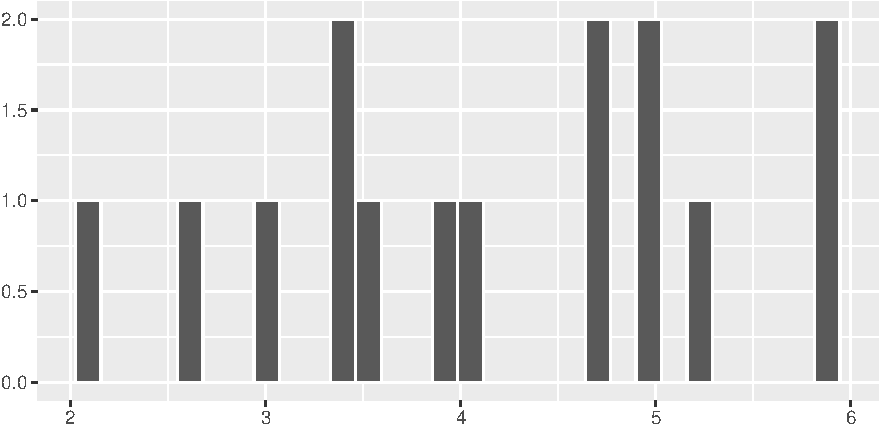
\includegraphics{inferencia_com_R_files/figure-latex/unnamed-chunk-51-1} \end{center}

Nessa simulação obtivemos a média das variâncias igual a 4.17 e a variância das variâncias igual a 1.33.

Suponha agora que façamos o mesmo processo, porém ao invés de considerarmos 15 amostras de tamanho 20, consideramos 1000 amostras.

\begin{Shaded}
\begin{Highlighting}[]
\NormalTok{n }\OtherTok{=} \DecValTok{1000}
\NormalTok{matriz\_aux }\OtherTok{=} \FunctionTok{matrix}\NormalTok{(}\ConstantTok{NA}\NormalTok{,}\AttributeTok{nrow=}\DecValTok{20}\NormalTok{,}\AttributeTok{ncol=}\NormalTok{n)}
\ControlFlowTok{for}\NormalTok{(j }\ControlFlowTok{in} \DecValTok{1}\SpecialCharTok{:}\FunctionTok{ncol}\NormalTok{(matriz\_aux))\{matriz\_aux[,j]}\OtherTok{=}\FunctionTok{rnorm}\NormalTok{(}\DecValTok{20}\NormalTok{,}\AttributeTok{mean=}\DecValTok{10}\NormalTok{,}\AttributeTok{sd=}\DecValTok{2}\NormalTok{)\}}
\NormalTok{variancias }\OtherTok{=} \FunctionTok{data.frame}\NormalTok{(}\AttributeTok{x=}\DecValTok{1}\SpecialCharTok{:}\FunctionTok{ncol}\NormalTok{(matriz\_aux),}\AttributeTok{y=}\FunctionTok{apply}\NormalTok{(matriz\_aux,}\DecValTok{2}\NormalTok{,var))}
\FunctionTok{ggplot}\NormalTok{(variancias,}\FunctionTok{aes}\NormalTok{(y)) }\SpecialCharTok{+}
  \FunctionTok{geom\_histogram}\NormalTok{(}\AttributeTok{color =} \StringTok{"white"}\NormalTok{) }\SpecialCharTok{+}
  \FunctionTok{theme}\NormalTok{(}\AttributeTok{axis.title =} \FunctionTok{element\_blank}\NormalTok{())}
\end{Highlighting}
\end{Shaded}

\begin{center}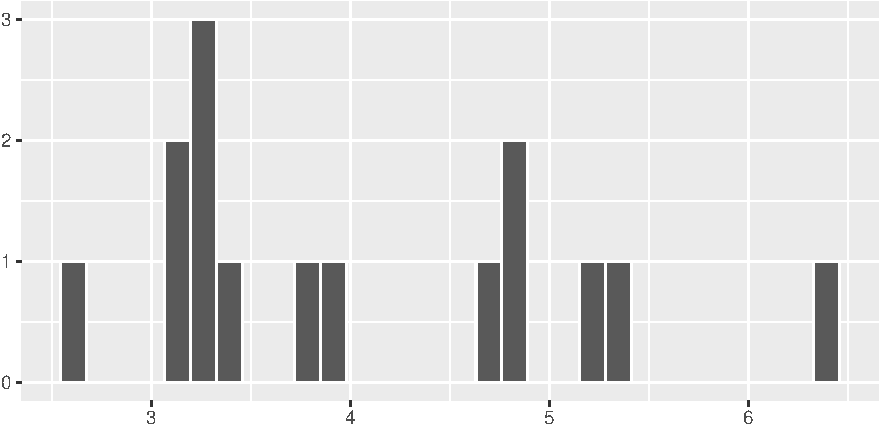
\includegraphics{inferencia_com_R_files/figure-latex/unnamed-chunk-52-1} \end{center}

Neste caso a média das variâncias foi igual a 3.99 e a variância das variâncias igual a 1.69.

Realizando o mesmo experimento, porém agora considerando 10000 amostras de tamanho 20, a distribuição da variância amostral pode ser vista segundo o histograma abaixo.

\begin{Shaded}
\begin{Highlighting}[]
\NormalTok{n }\OtherTok{=} \DecValTok{10000}
\NormalTok{matriz\_aux }\OtherTok{=} \FunctionTok{matrix}\NormalTok{(}\ConstantTok{NA}\NormalTok{,}\AttributeTok{nrow=}\DecValTok{20}\NormalTok{,}\AttributeTok{ncol=}\NormalTok{n)}
\ControlFlowTok{for}\NormalTok{(j }\ControlFlowTok{in} \DecValTok{1}\SpecialCharTok{:}\FunctionTok{ncol}\NormalTok{(matriz\_aux))\{matriz\_aux[,j]}\OtherTok{=}\FunctionTok{rnorm}\NormalTok{(}\DecValTok{20}\NormalTok{,}\AttributeTok{mean=}\DecValTok{10}\NormalTok{,}\AttributeTok{sd=}\DecValTok{2}\NormalTok{)\}}
\NormalTok{variancias }\OtherTok{=} \FunctionTok{data.frame}\NormalTok{(}\AttributeTok{x=}\DecValTok{1}\SpecialCharTok{:}\FunctionTok{ncol}\NormalTok{(matriz\_aux),}\AttributeTok{y=}\FunctionTok{apply}\NormalTok{(matriz\_aux,}\DecValTok{2}\NormalTok{,var))}
\FunctionTok{ggplot}\NormalTok{(variancias,}\FunctionTok{aes}\NormalTok{(y)) }\SpecialCharTok{+}
  \FunctionTok{geom\_histogram}\NormalTok{(}\AttributeTok{color =} \StringTok{"white"}\NormalTok{) }\SpecialCharTok{+}
  \FunctionTok{theme}\NormalTok{(}\AttributeTok{axis.title =} \FunctionTok{element\_blank}\NormalTok{())}
\end{Highlighting}
\end{Shaded}

\begin{center}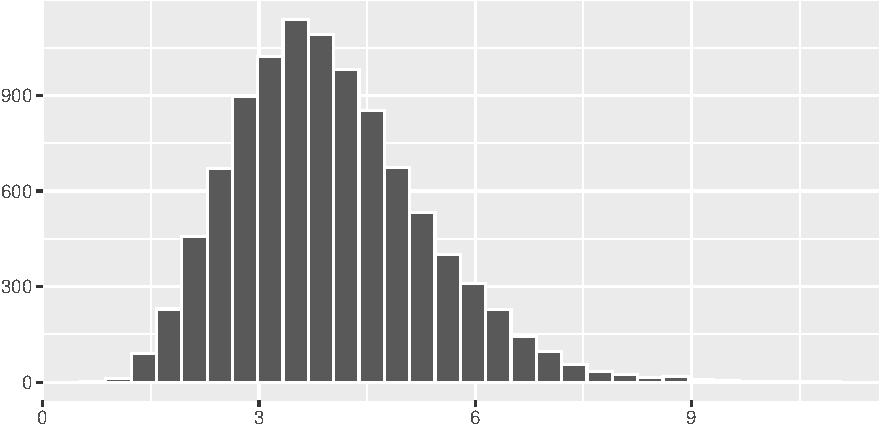
\includegraphics{inferencia_com_R_files/figure-latex/unnamed-chunk-53-1} \end{center}

Neste caso, a média das variâncias é 3.98 e a variância é 1.73. Então, realmente, podemos perceber que a distribuição da variância amostral se aproxima de uma distribuição qui-quadrado com média \(\mu=4\) e variância \(\frac{2\sigma^4}{n-1}=\frac{2\times 16}{19}=1,684\).

Destas propriedades temos que \[V(S^2)=\frac{2\sigma^4}{n-1}.\]

\hypertarget{distribuiuxe7uxe3o-amostral-da-proporuxe7uxe3o}{%
\section{Distribuição Amostral da Proporção}\label{distribuiuxe7uxe3o-amostral-da-proporuxe7uxe3o}}

Considere uma população em que cada elemento é classificado de acordo com a presença ou ausência de determinada característica. Por exemplo, podemos pensar em eleitores escolhendo entre 2 candidatos, pessoas classificadas de acordo com o sexo, trabalhadores classificados como trabalhador com carteira assinada ou não, e assim por diante. Em termos de variável aleatória, essa população é representada por uma v.a. de Bernoulli, isto é:

\[
X=\begin{cases}
1,~\text{se elemento possui a característica de interesse}\\
0,~\text{se elemento não possui a caracaterística de interesse}
\end{cases}
\]

Vamos denotar por \(p\) a proporção de elementos da população que possuem a característica de interesse. Então, \(P(X = 1) = p\), \(E(X) = p\) e \(V(X) = p(1 -p)\). Em geral, esse parâmetro é desconhecido e precisamos estimá-lo a partir de uma amostra.

Suponha, então, que dessa população seja extraída uma amostra aleatória simples \(X_1, X_2, \ldots , X_n\) com reposição. Essas \(n\) extrações correspondem a \(n\) variáveis aleatórias de Bernoulli independentes e, como sabemos, \(S_n =\sum_{i=1}^n X_i\) tem distribuição binomial com parâmetros \(n\) e \(p\).

Note que \(S_n\) dá o número total de ``sucessos'' nas \(n\) repetições, onde ``sucesso'', neste caso, representa a presença da característica de interesse. Os valores possíveis de \(S_n\) são \(0, 1, 2,\ldots , n\). Com relação à proporção \(\hat P\) de elementos na amostra que possuem a característica de interesse, temos que

\[\hat P = \frac{S_n}{n}=\frac{X_1+X_2+\ldots+X_n}{n}\]

e os valores possíveis de \(\hat P\) são \(0,\frac{1}{n},\frac{2}{n},\ldots,\frac{n-1}{n},1\) com

\[P\left(\hat P = \frac{k}{n}\right)=P(S_n=k).\]
Como a proporção amostral é uma média de uma amostra aleatória simples de uma população com distribuição de Bernoulli com parâmetro \(p\), o Teorema Limite Central nos diz, então, que a distribuição da proporção amostral se aproxima de uma normal com média \(p\) e variância \(\frac{p(1-p)}{n}\). Isto é,

\[\hat p \sim N\left(p,\frac{p(1-p)}{n}\right).\]

Como essa aproximação é uma conseqüência direta da aproximação normal da binomial, as mesmas regras continuam valendo: a aproximação deve ser feita se \(np \geq 5\) e \(n(1 - p) \geq 5\).

\hypertarget{visualizando-3}{%
\subsection{Visualizando}\label{visualizando-3}}

Considere uma população bernoulli com \(p=0,3\). Vamos realizar um estudo de simulação para a distribuição da proporção amostral considerando amostras de tamanho 20 dessa população.

Primeiramente, considere que são retiradas 15 amostras de tamanho 20 dessa população.

\begin{Shaded}
\begin{Highlighting}[]
\FunctionTok{library}\NormalTok{(ggplot2)}
\NormalTok{n }\OtherTok{=} \DecValTok{15}
\NormalTok{matriz\_aux }\OtherTok{=} \FunctionTok{matrix}\NormalTok{(}\ConstantTok{NA}\NormalTok{,}\AttributeTok{nrow=}\DecValTok{20}\NormalTok{,}\AttributeTok{ncol=}\NormalTok{n)}
\ControlFlowTok{for}\NormalTok{(j }\ControlFlowTok{in} \DecValTok{1}\SpecialCharTok{:}\FunctionTok{ncol}\NormalTok{(matriz\_aux))\{matriz\_aux[,j]}\OtherTok{=}\FunctionTok{rbinom}\NormalTok{(}\DecValTok{20}\NormalTok{,}\DecValTok{1}\NormalTok{,}\AttributeTok{prob=}\FloatTok{0.3}\NormalTok{)\}}
\NormalTok{medias }\OtherTok{=} \FunctionTok{data.frame}\NormalTok{(}\AttributeTok{x=}\DecValTok{1}\SpecialCharTok{:}\FunctionTok{ncol}\NormalTok{(matriz\_aux),}\AttributeTok{y=}\FunctionTok{colMeans}\NormalTok{(matriz\_aux))}
\FunctionTok{ggplot}\NormalTok{(medias,}\FunctionTok{aes}\NormalTok{(y)) }\SpecialCharTok{+}
  \FunctionTok{geom\_histogram}\NormalTok{(}\AttributeTok{color =} \StringTok{"white"}\NormalTok{, }\AttributeTok{bins =} \DecValTok{15}\NormalTok{) }\SpecialCharTok{+}
  \FunctionTok{theme}\NormalTok{(}\AttributeTok{axis.title =} \FunctionTok{element\_blank}\NormalTok{())}
\end{Highlighting}
\end{Shaded}

\begin{center}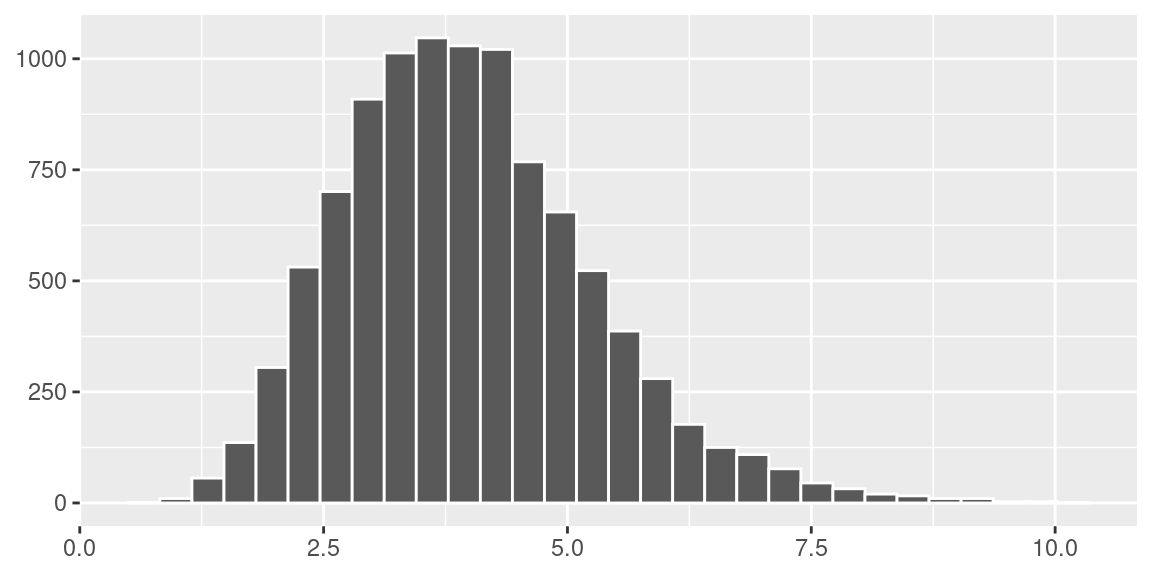
\includegraphics{inferencia_com_R_files/figure-latex/unnamed-chunk-54-1} \end{center}

Nessa simulação obtivemos \(\hat p =\) 0.32.

Suponha agora que façamos o mesmo processo, porém ao invés de considerarmos 15 amostras de tamanho 20, consideramos 200 amostras.

\begin{Shaded}
\begin{Highlighting}[]
\NormalTok{n }\OtherTok{=} \DecValTok{200}
\NormalTok{matriz\_aux }\OtherTok{=} \FunctionTok{matrix}\NormalTok{(}\ConstantTok{NA}\NormalTok{,}\AttributeTok{nrow=}\DecValTok{20}\NormalTok{,}\AttributeTok{ncol=}\NormalTok{n)}
\ControlFlowTok{for}\NormalTok{(j }\ControlFlowTok{in} \DecValTok{1}\SpecialCharTok{:}\FunctionTok{ncol}\NormalTok{(matriz\_aux))\{matriz\_aux[,j]}\OtherTok{=}\FunctionTok{rbinom}\NormalTok{(}\DecValTok{20}\NormalTok{,}\DecValTok{1}\NormalTok{,}\AttributeTok{prob=}\FloatTok{0.3}\NormalTok{)\}}
\NormalTok{medias }\OtherTok{=} \FunctionTok{data.frame}\NormalTok{(}\AttributeTok{x=}\DecValTok{1}\SpecialCharTok{:}\FunctionTok{ncol}\NormalTok{(matriz\_aux),}\AttributeTok{y=}\FunctionTok{colMeans}\NormalTok{(matriz\_aux))}
\FunctionTok{ggplot}\NormalTok{(medias,}\FunctionTok{aes}\NormalTok{(y)) }\SpecialCharTok{+}
  \FunctionTok{geom\_histogram}\NormalTok{(}\AttributeTok{color =} \StringTok{"white"}\NormalTok{, }\AttributeTok{bins =} \DecValTok{15}\NormalTok{) }\SpecialCharTok{+}
  \FunctionTok{theme}\NormalTok{(}\AttributeTok{axis.title =} \FunctionTok{element\_blank}\NormalTok{())}
\end{Highlighting}
\end{Shaded}

\begin{center}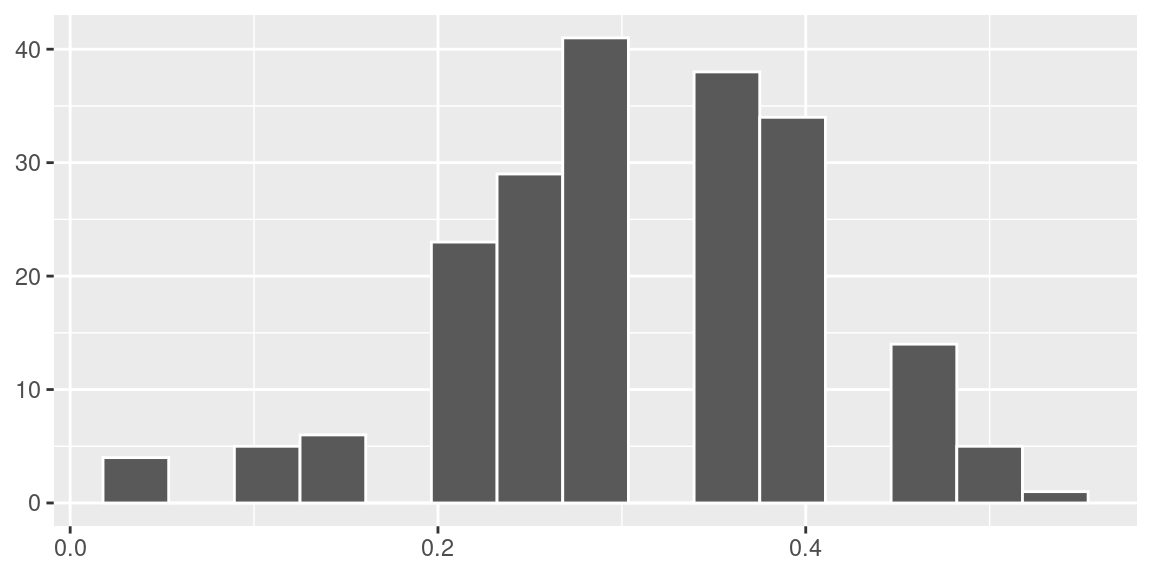
\includegraphics{inferencia_com_R_files/figure-latex/unnamed-chunk-55-1} \end{center}

Agora, obtivemos \(\hat p =\) 0.3.

Realizando o mesmo experimento, porém agora considerando 10000 amostras de tamanho 20, a distribuição da média amostral pode ser vista segundo o histograma abaixo.

\begin{Shaded}
\begin{Highlighting}[]
\NormalTok{n }\OtherTok{=} \DecValTok{10000}
\NormalTok{matriz\_aux }\OtherTok{=} \FunctionTok{matrix}\NormalTok{(}\ConstantTok{NA}\NormalTok{,}\AttributeTok{nrow=}\DecValTok{20}\NormalTok{,}\AttributeTok{ncol=}\NormalTok{n)}
\ControlFlowTok{for}\NormalTok{(j }\ControlFlowTok{in} \DecValTok{1}\SpecialCharTok{:}\FunctionTok{ncol}\NormalTok{(matriz\_aux))\{matriz\_aux[,j]}\OtherTok{=}\FunctionTok{rbinom}\NormalTok{(}\DecValTok{20}\NormalTok{,}\DecValTok{1}\NormalTok{,}\AttributeTok{prob=}\FloatTok{0.3}\NormalTok{)\}}
\NormalTok{medias }\OtherTok{=} \FunctionTok{data.frame}\NormalTok{(}\AttributeTok{x=}\DecValTok{1}\SpecialCharTok{:}\FunctionTok{ncol}\NormalTok{(matriz\_aux),}\AttributeTok{y=}\FunctionTok{colMeans}\NormalTok{(matriz\_aux))}
\FunctionTok{ggplot}\NormalTok{(medias,}\FunctionTok{aes}\NormalTok{(y)) }\SpecialCharTok{+}
  \FunctionTok{geom\_histogram}\NormalTok{(}\AttributeTok{color =} \StringTok{"white"}\NormalTok{, }\AttributeTok{bins =} \DecValTok{15}\NormalTok{) }\SpecialCharTok{+}
  \FunctionTok{theme}\NormalTok{(}\AttributeTok{axis.title =} \FunctionTok{element\_blank}\NormalTok{())}
\end{Highlighting}
\end{Shaded}

\begin{center}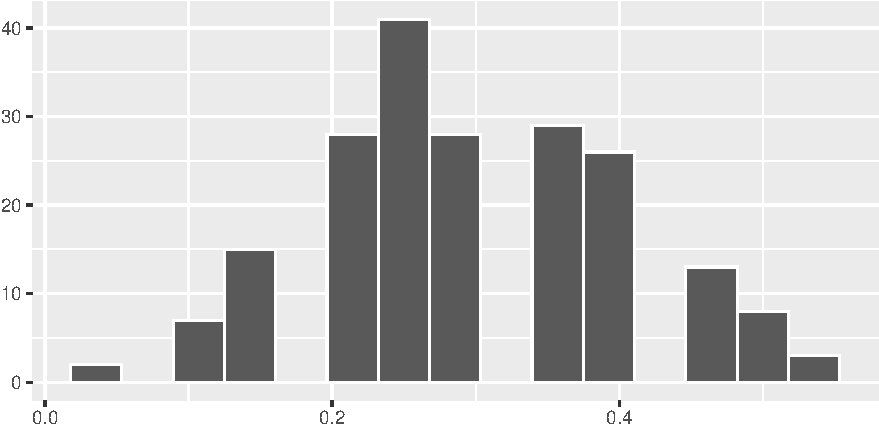
\includegraphics{inferencia_com_R_files/figure-latex/unnamed-chunk-56-1} \end{center}

Para este caso, a média das proporções amostrais foi \(\hat p=\) 0.3. Então, empiricamente, podemos perceber que a distribuição da média amostral se aproxima de uma distribuição normal com média \(\mu=0,3\) e desvio padrão \(\frac{p(1-p)}{\sqrt{n}}=\frac{0.21}{\sqrt{20}}=0,0105\).

\hypertarget{intervalo-de-confianuxe7a}{%
\chapter{Intervalo de Confiança}\label{intervalo-de-confianuxe7a}}

\hypertarget{introduuxe7uxe3o-4}{%
\section{Introdução}\label{introduuxe7uxe3o-4}}

Neste capítulo você aprenderá um método muito importante de estimação de parâmetros. Vimos anteriormente que a média amostral \(\bar X\) é um bom estimador da média populacional \(\mu\). Mas vimos, também, que existe uma variabilidade nos valores de \(\bar X\), ou seja, cada amostra dá origem a um valor diferente do estimador. Uma maneira de informar sobre esta variabilidade é através da estimação por intervalos.

\hypertarget{ideias-buxe1sicas}{%
\section{Ideias Básicas}\label{ideias-buxe1sicas}}

O objetivo central da Inferência Estatística é obter informações para uma população a partir do conhecimento de uma única amostra. Em geral, a população é representada por uma variável aleatória \(X\), com função de distribuição ou densidade de probabilidade \(f_X\) . Dessa população, então, extrai-se uma amostra aleatória simples com reposição, que dá origem a um conjunto \(X_1, X_2, \ldots, X_n\) de \(n\) variáveis aleatórias independentes e identicamente distribuídas, todas com a mesma distribuição \(f_X\).

Se \(f_X\) depende de um ou mais parâmetros, temos que usar a informação obtida a partir da amostra para estimar esses parâmetros, de forma a conhecermos a distribuição. Vimos, por exemplo, que a média amostral \(\bar X\) é um bom estimador da média populacional \(\mu\), no sentido de que ela tende a ``acertar o alvo'' da verdadeira média populacional, isto é, a média amostral é um estimador não-viesado da média populacional. Mas vimos, também, que existe uma variabilidade nos valores de \(\bar X\), ou seja, cada amostra dá origem a um valor diferente do estimador. Para algumas amostras, \(\bar X\) será maior que \(\mu\), para outras será menor e para outras será igual.

Na prática, temos apenas uma amostra e, assim, é importante que se dê alguma informação sobre essa possível variabilidade do estimador. Ou seja, é importante informar o valor do estimador \(\hat \theta\) obtido com uma amostra específica, mas é importante informar também que o verdadeiro valor do parâmetro \(\theta\) poderia estar num determinado intervalo, digamos, no intervalo \(\left[\hat\theta-\varepsilon,\hat\theta+\varepsilon\right]\). Dessa forma, estamos informando a nossa margem de erro no processo de estimação; essa margem de erro é consequência do processo de seleção aleatória da amostra.

O que vamos estudar agora é como obter esse intervalo, de modo a ``acertar na maioria das vezes'', isto é, queremos um procedimento que garanta que, na maioria das vezes (ou das amostras possíveis), o intervalo obtido conterá o verdadeiro valor do parâmetro. A expressão ``na maioria das vezes'' será traduzida como ``probabilidade alta''. Dessa forma, estaremos lidando com afirmativas do seguinte tipo:

\textbf{Com probabilidade alta (em geral, indicada por $1-\alpha$), o intervalo $\left[\hat\theta-\varepsilon,\hat\theta+\varepsilon\right]$ conterá o verdadeiro valor do parâmetro $\theta$.}

A interpretação correta de tal afirmativa é a seguinte: se \(1-\alpha=0,95\), por exemplo, então isso significa que o procedimento de construção do intervalo é tal que, em 95\% das possíveis amostras, o intervalo \(\left[\hat\theta-\varepsilon,\hat\theta+\varepsilon\right]\) obtido conterá o verdadeiro valor do parâmetro.

Note, no exemplo abaixo, que cada amostra resulta em um intervalo diferente, mas em média, em 95\% das amostras, o intervalo contém o verdadeiro valor do parâmetro (em vermelho).

\begin{center}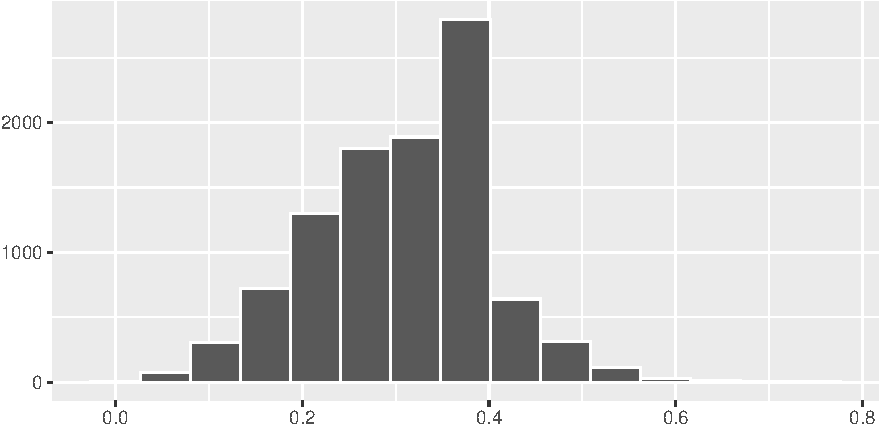
\includegraphics{inferencia_com_R_files/figure-latex/unnamed-chunk-57-1} \end{center}

O valor \(1 - \alpha\) é chamado nível de confiança, enquanto o valor \(\alpha\) é conhecido como nível de significância. O intervalo \(\left[\hat\theta-\varepsilon;\hat\theta + \varepsilon\right]\) é chamado de intervalo de confiança de nível de confiança \(1 - \alpha\).

Tendo clara a interpretação do intervalo de confiança, podemos resumir a frase acima da seguinte forma:

\[P\left(\theta\in[\hat\theta-\varepsilon;\hat\theta+\varepsilon]\right)=1-\alpha\]

Mais uma vez, a probabilidade se refere à probabilidade dentre as diversas possíveis amostras, ou seja, a probabilidade está associada à distribuição amostral de \(\hat \theta\). Note que os limites do intervalo dependem de \(\hat theta\), que depende da amostra sorteada, ou seja, os limites do intervalo de confiança são variáveis aleatórias. Cada amostra dá origem a um intervalo diferente, mas o procedimento de obtenção dos intervalos garante probabilidade \(1 - \alpha\) de acerto.

\hypertarget{muxe9dia-da-nmusigma2-sigma2-conhecido}{%
\section{\texorpdfstring{Média da \(N(\mu,\sigma^2)\), \(\sigma^2\) conhecido}{Média da N(\textbackslash mu,\textbackslash sigma\^{}2), \textbackslash sigma\^{}2 conhecido}}\label{muxe9dia-da-nmusigma2-sigma2-conhecido}}

Vamos agora introduzir os métodos para obtenção do intervalo de confiança para a média de uma população. Como visto, a média populacional é um parâmetro importante que pode ser muito bem estimado pela média amostral \(\bar X\). Para apresentar as idéias básicas, vamos considerar um contexto que é pouco frequente na prática. O motivo para isso é que, em termos didáticos, a apresentação é bastante simples. Como o fundamento é o mesmo para contextos mais gerais, essa abordagem se justifica.

Consideremos uma população descrita por uma variável aleatória normal com média \(\mu\) e variância \(\sigma^2\): \(X\sim N(\mu,\sigma^2)\). Vamos supor que o valor de \(\sigma^2\) seja conhecido e que nosso interesse seja estimar a média \(\mu\) a partir de uma amostra aleatória simples \(X_1,\ldots,X_n\). Como visto anteriormente, a distribuição amostral de \(\bar X\) é normal com média \(\mu\) e variância \(\frac{\sigma^2}{n}\), ou seja

\[X\sim N(\mu,\sigma^2)\rightarrow \bar X \sim N\left(\mu,\frac{\sigma^2}{n}\right)\]

Da definição de distribuição amostral, isso significa que os diferentes valores de \(\bar X\) obtidos a partir das diferentes possíveis amostras se distribuem normalmente em torno de \(\mu\) com variância \(\frac{\sigma^2}{n}\).

Das propriedades da distribuição normal, resulta que

\[Z=\frac{\bar X-\mu}{\sqrt{\frac{\sigma^2}{n}}}\sim N(0,1),\]

ou equivalentemente,

\[Z=\sqrt{n}\frac{\bar X-\mu}{\sigma}\sim N(0,1).\]

\hypertarget{notauxe7uxe3o}{%
\subsection{Notação}\label{notauxe7uxe3o}}

Vamos estabelecer a seguinte notação: vamos indicar por \(z_\alpha\) a abscissa da curva normal padrão que deixa probabilidade (área) igual a \(\alpha\) acima dela. Veja a Figura abaixo. Temos, então, que \(P(Z > z_\alpha)= \alpha\). Essa abscissa \(z_\alpha\) é normalmente chamada de valor crítico.

\begin{center}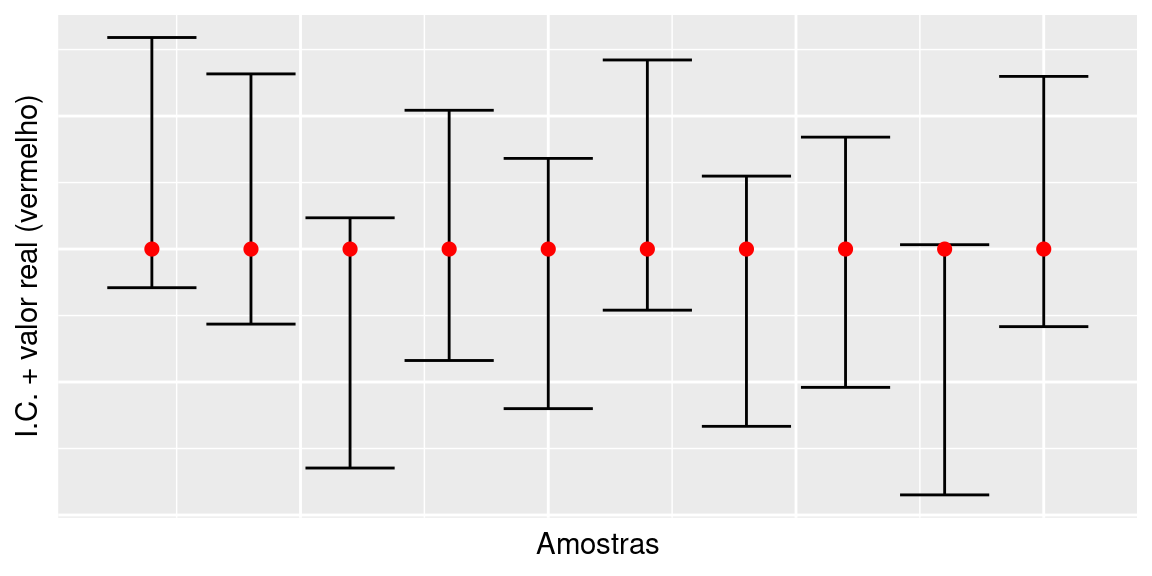
\includegraphics{inferencia_com_R_files/figure-latex/unnamed-chunk-58-1} \end{center}

Consideremos, agora, o valor crítico \(z_\frac{\alpha}{2}\), veja a Figura abaixo. Daí podemos ver que, se \(Z\sim N(0,1)\), então

\[P\left(-z_\frac{\alpha}{2}\leq Z \leq z_\frac{\alpha}{2}\right)=1-\alpha\]

\begin{center}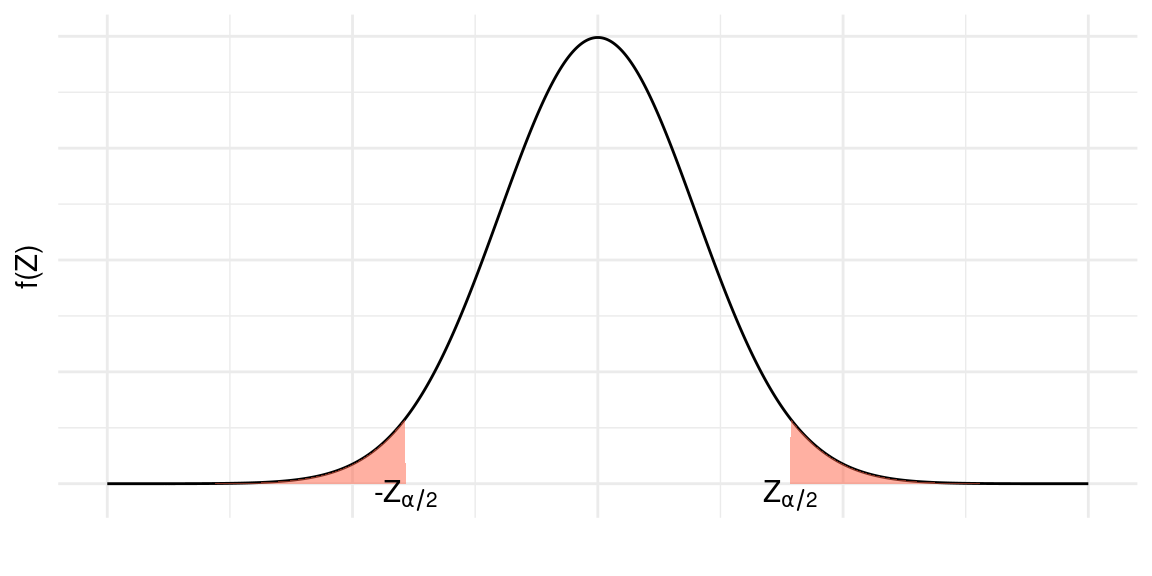
\includegraphics{inferencia_com_R_files/figure-latex/unnamed-chunk-59-1} \end{center}

Note que isso vale para a distribuição normal padrão, em geral. Então, usando os resultados anteriories obtemos que

\[P\left(-z_\frac{\alpha}{2}\leq \sqrt{n}\frac{\bar X-\mu}{\sigma} \leq z_\frac{\alpha}{2}\right)=1-\alpha\]

Mas isso é equivalente a

\[P\left(-z_{\frac{\alpha}{2}}\frac{\sigma}{\sqrt{n}}\leq \bar X-\mu \leq z_{\frac{\alpha}{2}}\frac{\sigma}{\sqrt{n}}\right)= 1-\alpha\]

\[P\left(-\bar X-z_{\frac{\alpha}{2}}\frac{\sigma}{\sqrt{n}}\leq -\mu \leq -\bar X + z_{\frac{\alpha}{2}}\frac{\sigma}{\sqrt{n}}\right)= 1-\alpha\]

\[P\left(\bar X - z_{\frac{\alpha}{2}}\frac{\sigma}{\sqrt{n}} \leq \mu \leq \bar X+z_{\frac{\alpha}{2}}\frac{\sigma}{\sqrt{n}}\right) = 1-\alpha\]

Note que a última expressão nos diz que

\[P\left(\mu \in \left[\bar X-z_{\frac{\alpha}{2}}\frac{\sigma}{\sqrt{n}};\bar X+z_{\frac{\alpha}{2}}\frac{\sigma}{\sqrt{n}}\right]\right)=1-\alpha\]

Mas essa é exatamente a forma geral de um intervalo de confiança, conforme explicitado. Temos, então, a seguinte conclusão:

Seja \(X\sim N(\mu, \sigma^2)\) uma população normal com variância \(\sigma^2\) conhecida. Se \(X_1, X_2,\ldots , X_n\) é uma amostra aleatória dessa população, então o intervalo de confiança de nível de confiança \(1-\alpha\) para a média populacional \(\mu\) é dado por

\[\left[\bar X-z_{\frac{\alpha}{2}}\frac{\sigma}{\sqrt{n}};\bar X+z_{\frac{\alpha}{2}}\frac{\sigma}{\sqrt{n}}\right],\]

onde \(z_{\frac{\alpha}{2}}\) é a abcissa da curva normal padrão que deixa a área \(\frac{\alpha}{2}\) acima dela.

\hypertarget{margem-de-erro}{%
\section{Margem de Erro}\label{margem-de-erro}}

O intervalo de confiança para \(\mu\) pode ser escrito na forma \(\left[\bar X - \varepsilon;\bar X + \varepsilon \right]\) onde \(\varepsilon=z_{\frac{\alpha}{2}}\frac{\sigma}{\sqrt{n}}\) é a margem de erro.

Analisando a margem de erro, podemos ver que ela depende diretamente do valor crítico e do desvio padrão populacional e é inversamente proporcional ao tamanho da amostra.

Na Figura abaixo ilustra-se a relação de dependência da margem de erro em relação ao desvio padrão populacional \(\sigma\). Temos aí duas distribuições amostrais centradas na mesma média e baseadas em amostras de mesmo tamanho. Nas duas distribuições a área total das caudas sombreadas é \(\alpha\), de modo que o intervalo limitado pelas linhas verticais é o intervalo de confiança de nível de confiança \(1-\alpha\). Para a distribuição mais dispersa, isto é, com \(\sigma\) maior, o comprimento do intervalo é maior. Esse resultado deve ser intuitivo: se há mais variabilidade na população, a nossa margem de erro tem que ser maior, mantidas fixas as outras condições (tamanho de amostra e nível de confiança).

\begin{center}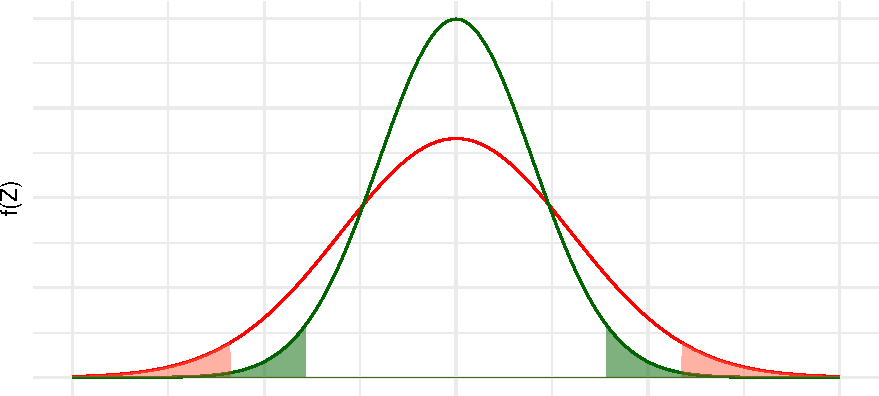
\includegraphics{inferencia_com_R_files/figure-latex/unnamed-chunk-60-1} \end{center}

Por outro lado, se mantivermos fixos o tamanho da amostra e o desvio padrão populacional, é razoável também esperar que a margem de erro seja maior para um nível de confiança maior. Ou seja, se queremos aumentar a probabilidade de acerto, é razoável que o intervalo seja maior. Aumentar a probabilidade de acerto significa aumentar o nível de confiança, o que acarreta em um valor crítico \(z_{\frac{\alpha}{2}}\) maior.

Finalmente, mantidos o mesmo desvio padrão populacional e o mesmo nível de confiança, quanto maior o tamanho da amostra, mais perto vamos ficando da população e, assim, vai diminuindo a nossa margem de erro.

\hypertarget{introduuxe7uxe3o-5}{%
\section{Introdução}\label{introduuxe7uxe3o-5}}

Neste capítulo você completará seu estudo básico sobre intervalos de confiança para a média de uma população, analisando o problema de estimação da média de uma população normal quando não se conhece a variância desta população. Você verá que, neste caso, é necessário estimar essa variância e isso introduz mais uma fonte de variabilidade nas nossas estimativas: com uma única amostra, temos que estimar a média e a variância da população. O procedimento é simples e análogo aos casos anteriores vistos nos capítulos amteriores; o que muda é a distribuição amostral do estimador \(\bar X\). Em vez de usarmos a distribuição normal para determinar os valores críticos, usaremos a distribuição \(t\) de Student.

\hypertarget{ideias-buxe1sicas-1}{%
\section{Ideias Básicas}\label{ideias-buxe1sicas-1}}

Considere uma população descrita por uma variável aleatória normal com média \(\mu\) e variância \(\sigma^2\): \(X\sim N(\mu,\sigma^2)\). Nosso interesse é estimar a média \(\mu\) a partir de uma amostra aleatória simples \(X_1,X_2,\ldots,X_n\). Como visto anteriormente, a distribuição amostral de \(\bar X\) é normal com média \(\mu\) e variância \(\frac{\sigma^2}{n}\), ou seja

\[X\sim N(\mu,\sigma^2)\rightarrow \bar X \sim N\left(\mu,\frac{\sigma^2}{n}\right)\]
Asso, se o valor de \(\sigma\) é conhecido, resulta que

\[Z=\sqrt{n}\frac{\bar X-\mu}{\sigma}\sim N(0,1)\]

e esse resultado foi utilizado na construção do intervalo de confiança para a média de uma população normal com variância conhecida, fornecendo o seguinte intervalo:

\[\left[\bar X-z_{\frac{\alpha}{2}}\frac{\sigma}{\sqrt{n}};\bar X+z_{\frac{\alpha}{2}}\frac{\sigma}{\sqrt{n}}\right].\]

Suponhamos, agora, que a variância \(\sigma^2\) não seja conhecida. Neste caso, temos que estimá-la (\(S^2\)) com os dados amostrais. Foi demostrado que

\[S^2=\frac{1}{n-1}\sum_{i=1}^{n}(X_i-\bar X)^2=\frac{1}{n-1}\left[\sum_{i=1}^{n}X_i^2-n\bar X^2\right]\]

é um estimador não viesado para \(\sigma^2\). Isso significa que, se calculássemos o valor de \(S^2\) para cada uma das possíveis amostras aleatórias simples de tamanho \(n\), a média desses valores seria igual a \(\sigma^2\). Dessa forma, \(S^2\) é um ``bom'' estimador de \(\sigma^2\) e podemos usá-lo como uma estimativa pontual de \(\sigma^2\). Como o desvio padrão é a raiz quadrada da variância, é natural perguntar: \(S\) é um ``bom'' estimador de \(\sigma\), ou seja, \(S\) é um estimador não-viesado de \(\sigma\)? A resposta é NÃO, mas, para grandes amostras, o viés é pequeno, de modo que, em geral, usa-se \(S\) como estimador de \(\sigma\). Sendo assim, é natural pensarmos em substituir o valor de \(\sigma\) por \(S\) na expressão da Normal \(Z\) e utilizarmos a estatística

\[T=\sqrt{n}\frac{\bar X-\mu}{S}\]

na construção de intervalos de confiança para \(\mu\). Isso é exatamente o que faremos, mas, ao introduzirmos \(S\) no lugar de \(\sigma\), a distribuição amostral de \(T\) deixa de ser normal e passa a ser uma distribuição \(t\) de Student.

\hypertarget{muxe9dia-da-nmusigma2-sigma2-desconhecido}{%
\subsection{\texorpdfstring{Média da \(N(\mu,\sigma^2)\), \(\sigma^2\) desconhecido}{Média da N(\textbackslash mu,\textbackslash sigma\^{}2), \textbackslash sigma\^{}2 desconhecido}}\label{muxe9dia-da-nmusigma2-sigma2-desconhecido}}

O intervalo de confiança para a média de uma população normal com variância desconhecida é obtido com base no seguinte resultado:

\[T=\sqrt{n}\frac{\bar X-\mu}{S}\sim t_{n-1},\]

onde \(S^2=\frac{1}{n-1}\sum_{i=1}^{n}(X_i-\bar X)^2=\frac{1}{n-1}\left[\sum_{i=1}^{n}X_i^2-n\bar X^2\right].\)

O número de graus de liberdade \(gl=n-1\) resulta do fato de que, na soma que define \(S^2\), há apenas \(n-1\) parcelas independentes, ou seja, dados \(S^2\) e \(n-1\) das parcelas \((X_i - \bar X)^2\), a \(n\)-ésima parcela fica automaticamente determinada.

Usando a simetria da densidade \(t\), temos o seguinte resultado:

\[P\left(-t_{n,\alpha/2}\leq t_{n} \leq t_{n,\alpha/2}\right)=1-\alpha\]

\begin{center}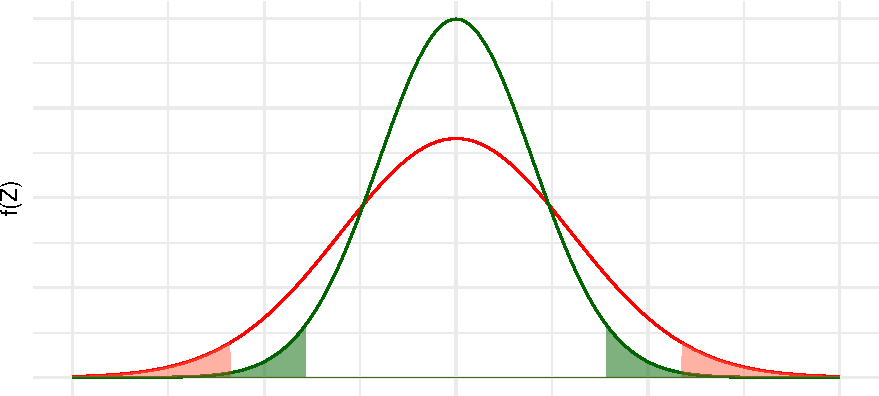
\includegraphics{inferencia_com_R_files/figure-latex/unnamed-chunk-61-1} \end{center}

Note que isso vale para a distribuição \(t\) de student, em geral. Então, usando os resultados anteriories obtemos que

\[P\left(-t_{n-1,\alpha/2}\leq \sqrt{n}\frac{\bar X-\mu}{S} \leq t_{n-1,\alpha/2}\right)=1-\alpha\]

Mas isso é equivalente a

\[P\left(-t_{n-1,\alpha/2}\frac{S}{\sqrt{n}}\leq \bar X-\mu \leq t_{n-1,\alpha/2}\frac{S}{\sqrt{n}}\right)=1-\alpha\]
\[P\left(\bar X-t_{n-1,\alpha/2}\frac{S}{\sqrt{n}}\leq \mu \leq \bar X + t_{n-1,\alpha/2}\frac{S}{\sqrt{n}}\right)=1-\alpha\]

Note que a última expressão nos diz que

\[P\left(\mu \in \left[\bar X-t_{n-1,\alpha/2}\frac{S}{\sqrt{n}};\bar X+t_{n-1,\alpha/2}\frac{S}{\sqrt{n}}\right]\right)=1-\alpha\]

Mas essa é exatamente a forma geral de um intervalo de confiança, conforme explicitado. Temos, então, a seguinte conclusão:

Seja \(X\sim N(\mu, \sigma^2)\) uma população normal com variância \(\sigma^2\) desconhecida. Se \(X_1, X_2,\ldots , X_n\) é uma amostra aleatória dessa população, então o intervalo de confiança de nível de confiança \(1-\alpha\) para a média populacional \(\mu\) é dado por

\[\left[\bar X-t_{n-1,\alpha/2}\frac{S}{\sqrt{n}};\bar X+t_{n-1,\alpha/2}\frac{S}{\sqrt{n}}\right],\]

onde \(t_{n-1,\alpha/2}\) é o valor crítico da distribuição \(t\) de student com \(n-1\) graus de liberdade que deixa a área \(\frac{\alpha}{2}\) acima dela.

\hypertarget{margem-de-erro-1}{%
\section{Margem de Erro}\label{margem-de-erro-1}}

Note, mais uma vez, a forma do intervalo de confiança:

\[\bar X \pm\varepsilon,\]

onde a margem de erro \(\varepsilon\), agora é definida em termos do valor crítico da distribuição \(t\) e do erro padrão estimado de \(\bar X\):

\[\varepsilon=t_{n-1,\alpha/2}\frac{S}{\sqrt{n}}\].

\hypertarget{introduuxe7uxe3o-6}{%
\section{Introdução}\label{introduuxe7uxe3o-6}}

Anteriormente, foram apresentadas as idéias básicas da estimação por intervalos de confiança. Para ilustrar o princípio utilizado na construção de tais intervalos, consideramos a situação especial de estimação da média de uma população normal com variância conhecida. Neste caso, a distribuição amostral da média amostral é normal e foi com base nessa distribuição amostral normal que obtivemos o intervalo de confiança.

No primeiro momento desta aula usaremos o teorema limite central, que garante que a distribuição amostral da proporção amostral pode ser aproximada por uma distribuição normal, desde que utilizemos amostras grandes.

\hypertarget{intervalo-de-confianuxe7a-para-a-proporuxe7uxe3o-populacional}{%
\section{Intervalo de confiança para a proporção populacional}\label{intervalo-de-confianuxe7a-para-a-proporuxe7uxe3o-populacional}}

\hypertarget{ideias-buxe1sicas-2}{%
\subsection{Ideias Básicas}\label{ideias-buxe1sicas-2}}

O contexto de interesse é o seguinte: temos uma população em que cada elemento é classificado de acordo com a presença ou ausência de determinada característica. Em termos de variável aleatória, essa população é representada por uma v.a. de Bernoulli, isto é:

\[
X=\begin{cases}
1,~\text{se elemento possui a característica de interesse}\\
0,~\text{se elemento não possui a caracaterística de interesse}
\end{cases}
\]

Então, \(P(X = 1) = p\), \(E(X) = p\) e \(V(X) = p(1 - p)\). O parâmetro \(p\) é também a proporção de elementos da população que possuem a caracterísitca de interesse. Em geral, esse parâmetro é desconhecido e precisamos estimá-lo a partir de uma amostra.

Suponha, então, que dessa população seja extraída uma amostra aleatória simples \(X_1, X_2, \ldots, X_n com reposição\). Vimos que a proporção \(\hat P\) de elementos na amostra que possuem a característica de interesse, definida por

\[\hat P = \frac{S_n}{n}=\frac{X_1+X_2+\ldots+X_n}{n}\]

é um estimador não-viesado para \(p\) com variância \(\frac{p(1-p)}{n}\). Mais precisamente,

\[E(\hat P)=p\]

\[V(\hat P)=\frac{p(1-p)}{n}\]

Como a proporção amostral é uma média de uma amostra aleatória simples de uma população com distribuição de Bernoulli com parâmetro \(p\), o Teorema Limite Central nos diz que a distribuição de \(\hat P\) se aproxima de uma nornal com média \(p\) e variância \(\frac{p(1-p)}{n}\).

Resumindo, temos o seguinte resultado:

\[\hat p \sim N\left(p,\frac{p(1-p)}{n}\right).\]

Usando as propriedades da distribuição normal, temos que

\[\frac{\hat P - p}{\sqrt{\frac{p(1-p)}{n}}}\sim N(0,1)\]

ou equivalentemente

\[\sqrt{n}\frac{\hat P - p}{\sqrt{p(1-p)}}\sim N(0,1)\]

Vamos ver, agora, como usar esse resultado para obter um intervalo de confiança para a verdadeira proporção populacional \(p\).

\hypertarget{construuxe7uxe3o-do-ic}{%
\subsection{Construção do IC}\label{construuxe7uxe3o-do-ic}}

O procedimento de construção do intervalo de confiança para a proporção populacional é totalmente análogo ao do intervalo de confiança para a média de uma população normal com variância conhecida, visto anteriormente. Assim, iremos usar a mesma notação, a saber: vamos representar por \(z_\alpha\) a abscissa da curva normal padrão que deixa probabilidade (área) \(\alpha\) acima dela. Como visto, temos o seguinte resultado, onde \(Z\sim N(0,1)\):

\[P\left(-z_\frac{\alpha}{2}\leq Z \leq z_\frac{\alpha}{2}\right)=1-\alpha\]

Como o resultado acima vale para qualquer variável aleatória \(N(0,1)\), podemos usar para obter

\[P\left(-z_{\frac{\alpha}{2}}\leq \frac{\hat P - p}{\sqrt{\frac{p(1-p)}{n}}} \leq z_{\frac{\alpha}{2}}\right)=1-\alpha\]

e, portanto

\[P\left(-z_{\frac{\alpha}{2}}\sqrt{\frac{p(1-p)}{n}} \leq \hat P - p \leq z_{\frac{\alpha}{2}}\sqrt{\frac{p(1-p)}{n}}\right)=1-\alpha\]

\[P\left(-\hat P -z_{\frac{\alpha}{2}}\sqrt{\frac{p(1-p)}{n}} \leq - p \leq -\hat P + z_{\frac{\alpha}{2}}\sqrt{\frac{p(1-p)}{n}}\right)=1-\alpha\]

\[P\left(\hat P - z_{\frac{\alpha}{2}}\sqrt{\frac{p(1-p)}{n}} \leq p \leq \hat P + z_{\frac{\alpha}{2}}\sqrt{\frac{p(1-p)}{n}}\right)=1-\alpha\]
Como no caso da média, chegamos a uma expressão do seguinte tipo:

\[P(\hat P -\varepsilon\leq p\leq\hat P + \varepsilon)=1-\alpha\]

onde \(\varepsilon=z_{\frac{\alpha}{2}}\sqrt{\frac{p(1-p)}{n}}\)

Analisando a margem de erro, podemos ver uma diferença fundamental entre o IC para a proporção e para a média: a margem de erro da proporção amostral depende do parâmetro desconhecido \(p\). Na prática, para construir o intervalo de confiança, temos que substituir esse valor por alguma estimativa.

Existem 3 abordagens possíveis:

\begin{enumerate}
\def\labelenumi{\arabic{enumi}.}
\item
  Usar a própria proporção amostral observada; nesse caso, o intervalo de confiança seria: \[\hat p \pm z_{\frac{\alpha}{2}}\sqrt{\frac{\hat p(1-\hat p)}{n}}\]
\item
  Usar o intervalo de confiança conservador, ou seja, usar o maior valor possível para \(z_{\frac{\alpha}{2}}\sqrt{\frac{\hat p(1-\hat p)}{n}}\) para um dado \(n\), o que equivale a obter o intervalo de confiança com o maior comprimento possível. Como o comprimento do intervalo é diretamente proporcional a \(\sqrt{p(1-p)}\) ou equivalentemente a \(p(1-p)\), \(p=0.5\) maxima esta função.
\end{enumerate}

Neste caso, o o intervalo de confiança se torna:

\[\hat p \pm z_{\frac{\alpha}{2}}\sqrt{\frac{0.5\times 0.5}{n}} = \hat p \pm z_{\frac{\alpha}{2}}\frac{0.5}{\sqrt{n}}\]

\begin{enumerate}
\def\labelenumi{\arabic{enumi}.}
\setcounter{enumi}{2}
\tightlist
\item
  Usar algum valor auxiliar \(\hat p_0\) ou estimativa prévia, obtida de outras fontes ou de uma amostra piloto:
\end{enumerate}

\[\hat p \pm z_{\frac{\alpha}{2}}\sqrt{\frac{\hat p_0(1-\hat p_0)}{n}}\]

Seja \(X\sim Bernoulli(p)\). Se \(X_1,X_2,\ldots,X_n\) é uma amostra aleatória dessa população, então o intervalo de confiança de nível de confiança \(1-\alpha\) para a proporção populacional \(p\) é dado por

\[\left[\hat P - z_{\frac{\alpha}{2}}\sqrt{\frac{\hat p_0(1-\hat p_0)}{n}};\hat P + z_{\frac{\alpha}{2}}\sqrt{\frac{\hat p_0(1-\hat p_0)}{n}}\right],\]

onde \(z_{\frac{\alpha}{2}}\) é a abcissa da curva normal padrão que deixa a área \(\frac{\alpha}{2}\) acima dela e \(\hat p_0\) é alguma estimativa para o verdadeiro valor de \(p\).

\hypertarget{determinauxe7uxe3o-do-tamanho-da-amostra}{%
\subsection{Determinação do tamanho da amostra}\label{determinauxe7uxe3o-do-tamanho-da-amostra}}

Uma questão que se coloca freqüentemente é: qual o tamanho da amostra necessário para se estimar uma proporção \(p\) com uma margem de erro \(\varepsilon\) e nível de confiança \(1-\alpha\)? Vamos analisar a expressão da margem de erro:

\[\varepsilon=z_{\frac{\alpha}{2}}\sqrt{\frac{p(1-p)}{n}}\]

Resolvendo para \(n\), obtemos que

\[\sqrt{n}=z_{\frac{\alpha}{2}}\frac{\sqrt{p(1-p)}}{\varepsilon}\]

ou

\[n=p(1-p)\left(\frac{z_{\frac{\alpha}{2}}}{\varepsilon}\right)^2\]

Vemos, então, que \(n\) é diretamente proporcional a \(p(1-p)\), ou seja, quanto maior \(p(1-p)\), maior será o tamanho da amostra \(n\). Na prática, não conhecemos \(p\) (na verdade, estamos querendo estimar esse parâmetro). Então, para determinar o tamanho de amostra necessário para uma margem de erro e um nível de confiança dados, podemos considerar o pior caso, ou seja, podemos tomar o maior valor possível de \(p(1 - p)\) e calcular o tamanho da amostra com base nesse pior caso, que ocorre quando \(p = 0,5\). É claro que essa é uma escolha conservadora, que em alguns casos pode levar a um tamanho de amostra desnecessariamente grande. Usando esta estimativa para \(p\), obtemos que

\[n=\left(0,5\times \frac{z_{\frac{\alpha}{2}}}{\varepsilon}\right)^2\]

\hypertarget{intervalo-de-confianuxe7a-para-a-variuxe2ncia-da-nmusigma2}{%
\section{\texorpdfstring{Intervalo de confiança para a variância da \(N(\mu,\sigma^2)\)}{Intervalo de confiança para a variância da N(\textbackslash mu,\textbackslash sigma\^{}2)}}\label{intervalo-de-confianuxe7a-para-a-variuxe2ncia-da-nmusigma2}}

Nesta parte você completará seu estudo básico sobre intervalos de confiança, analisando o problema de estimação da variância de uma população normal. Como antes, este intervalo se baseará na distribuição amostral de um estimador não-viesado para \(\sigma^2\), a saber, \(S^2\). Como a variância é um número não negativo, essa distribuição não é simétrica e está definida apenas para valores não-negativos.

\hypertarget{ideias-buxe1sicas-3}{%
\subsection{Ideias básicas}\label{ideias-buxe1sicas-3}}

O contexto subjacente é o seguinte: a partir de uma amostra aleatória simples \(X_1,X_2,\ldots,X_n\) retirada de uma população normal com média \(\mu\) e variância \(\sigma^2\) queremos construir um intervalo de confiança para \(\sigma^2\). A hipótese de normalidade da população é fundamental aqui. Assim como no caso da média, temos que usar a distribuição amostral de algum estimador. Neste caso, o estimador é \(S^2\) e o resultado importate é o seguinte: \(\frac{(n-1)S^2}{\sigma^2}\) tem distribuição qui-quadrado com \(n-1\) graus de liberdade:

\[\frac{(n-1)S^2}{\sigma^2}\sim\chi^2_{n-1}\]

\hypertarget{construuxe7uxe3o-do-ic-1}{%
\subsection{Construção do IC}\label{construuxe7uxe3o-do-ic-1}}

Como no caso da distribuição \(t\)-Student e também da distribuição Normal, vamos definir o valor crítico \(\chi^2_{n;\alpha}\) como a abscissa da distribuição qui-quadrado com \(n\) graus de liberdade que deixa probabilidade \(\alpha\) acima dela.

\begin{center}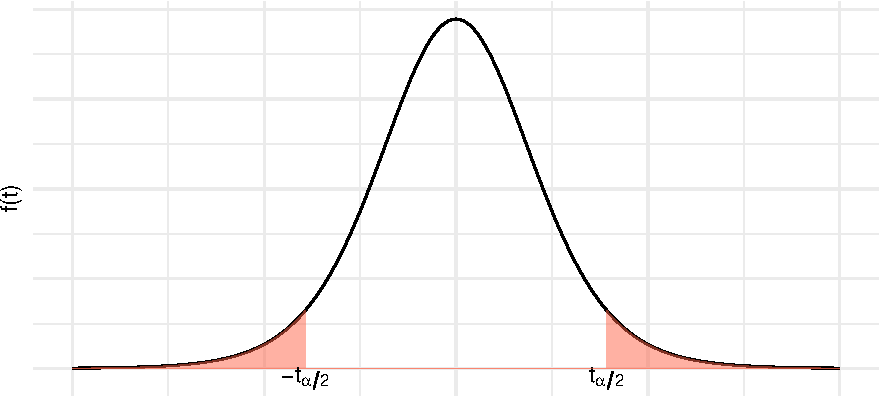
\includegraphics{inferencia_com_R_files/figure-latex/unnamed-chunk-62-1} \end{center}

Com essa definição, podemos ver que a abscissa \(\chi^2_{n;\alpha/2}\) deixa probabilidade \(\alpha/2\) acima dela e a abcissa \(\chi^2_{n;1-\alpha/2}\) deixa probabilidade \(\alpha/2\) abaixo dela.

\begin{center}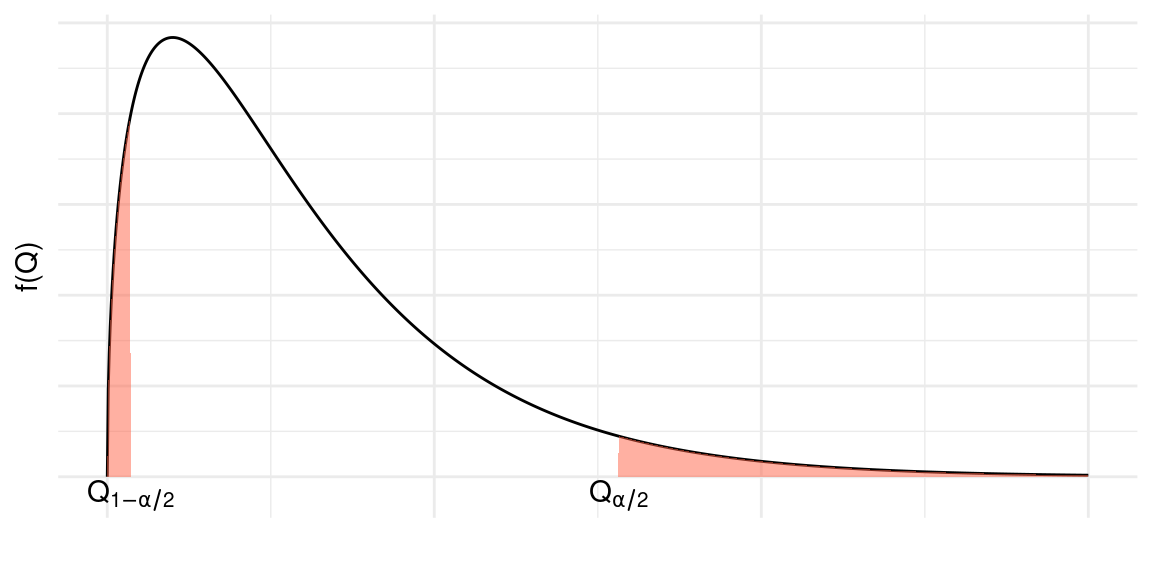
\includegraphics{inferencia_com_R_files/figure-latex/unnamed-chunk-63-1} \end{center}

Logo,

\[P\left(\chi^2_{n;\frac{\alpha}{2}}\leq \chi^2_{n} \leq \chi^2_{n;1-\frac{\alpha}{2}}\right)=1-\alpha\]

Como o resultado acima vale para qualquer distribuição qui-quadrado, podemos usar o resultado anterior para escrever

\[P\left(\chi^2_{n-1;\frac{\alpha}{2}}\leq \frac{(n-1)S^2}{\sigma^2} \leq \chi^2_{n-1;1-\frac{\alpha}{2}}\right)=1-\alpha\]

Daí resulta que

\[P\left(\frac{\chi^2_{n-1;\frac{\alpha}{2}}}{(n-1)S^2}\leq \frac{1}{\sigma^2} \leq \frac{\chi^2_{n-1;1-\frac{\alpha}{2}}}{(n-1)S^2}\right)=1-\alpha\]

\[P\left(\frac{(n-1)S^2}{\chi^2_{n-1;1-\frac{\alpha}{2}}}\leq \sigma^2 \leq \frac{(n-1)S^2}{\chi^2_{n-1;\frac{\alpha}{2}}}\right)=1-\alpha\]

e esse é o intervalo de confiança para a variância de uma população normal.

Seja \(X\sim N(\mu,\sigma^2)\) uma população normal. Se \(X_1,X_2,\ldots,X_n\) é uma amostra aleatória dessa população, então o intervalo de confiança de nível de confiança \(1-\alpha\) para a variância populacional \(\sigma^2\) é dado por

\[\left[\frac{(n-1)S^2}{\chi^2_{n-1;1-\frac{\alpha}{2}}};\frac{(n-1)S^2}{\chi^2_{n-1;\frac{\alpha}{2}}}\right],\]

onde \(\chi^2_{n-1;\frac{\alpha}{2}}\) é o valor crítico da distribuição qui-quadrado com \(n-1\) graus de liberdade que deixa a área \(\frac{\alpha}{2}\) abaixo dela e \(\chi^2_{n-1;1-\frac{\alpha}{2}}\) é o valor crítico da distribuição qui-quadrado com \(n-1\) graus de liberdade que deixa a área \(\frac{\alpha}{2}\) acima dela.

  \bibliography{book.bib,packages.bib}

\end{document}
